\documentclass[a4paper,12pt]{article}

% Работа с чешским языком
\usepackage{cmap}					          % поиск в PDF
\usepackage{mathtext} 				        % русские буквы в фомулах
\usepackage[T2A]{fontenc}		         % кодировка
\usepackage[utf8]{inputenc}			     % кодировка исходного текста
\usepackage[english,czech]{babel}	% локализация и переносы

% Работа с картинками
\usepackage{graphicx}  	   % Для вставки рисунков
\graphicspath{{images/}}  % папки с картинками
 
\usepackage{ulem}

\usepackage{hyperref}
\usepackage[usenames,dvipsnames,svgnames,table,rgb]{xcolor}
\hypersetup{				                                  % Гиперссылки
	unicode=true,                                            % русские буквы в раздела PDF
	pdftitle={Заголовок},                                % Заголовок
	pdfauthor={Автор},                                   % Автор
	pdfsubject={Тема},                                    % Тема
	pdfcreator={Создатель},                          % Создатель
	pdfproducer={Производитель},              % Производитель
	pdfkeywords={keyword1} {key2} {key3}, % Ключевые слова
	colorlinks=true,       	                                 % false: ссылки в рамках; true: цветные ссылки
	linkcolor=red,                                            % внутренние ссылки
	citecolor=green,                                        % на библиографию
	filecolor=magenta,                                    % на файлы
	urlcolor=blue                                             % на URL
}

\begin{document} 	  % конец преамбулы, начало документа

\thispagestyle{empty}
\begin{center}
	\textit{spol. s r.o.}
	\vspace{0.5ex}
	
	\textbf{VÝSOKÁ ŠKOLA HOTELOVÁ V PRAZE}
\end{center}
\vspace{13ex}

\begin{center}
	\vspace{13ex}
	\textbf{INFORMAČNÍ SYSTÉM VŠH}
	\vspace{1ex}
	
	\textbf{\textit{<<Krátká příručka>>}}
	
	\vfill
	
\includegraphics[width=0.5\textwidth]{logo}
	
	\vfill
	Praha 2014
\end{center}

\newpage

\section{Úvod}

Tato příručka se pomuže orientovat novým studentům v informačním systému VŠH 
a být dobře informováným studentem.

\vspace{15ex}
\textbf{TENTO DOKUMENT NENÍ OFICIÁLNÍ.}

\newpage

\section{Přihlásit se}

Pro přístup do informačního systému VŠH, musíte vytočit 
webový prohlížeč na adresu: \url{http://is.vsh.cz/}
Tam uvidíte následující obrázek:

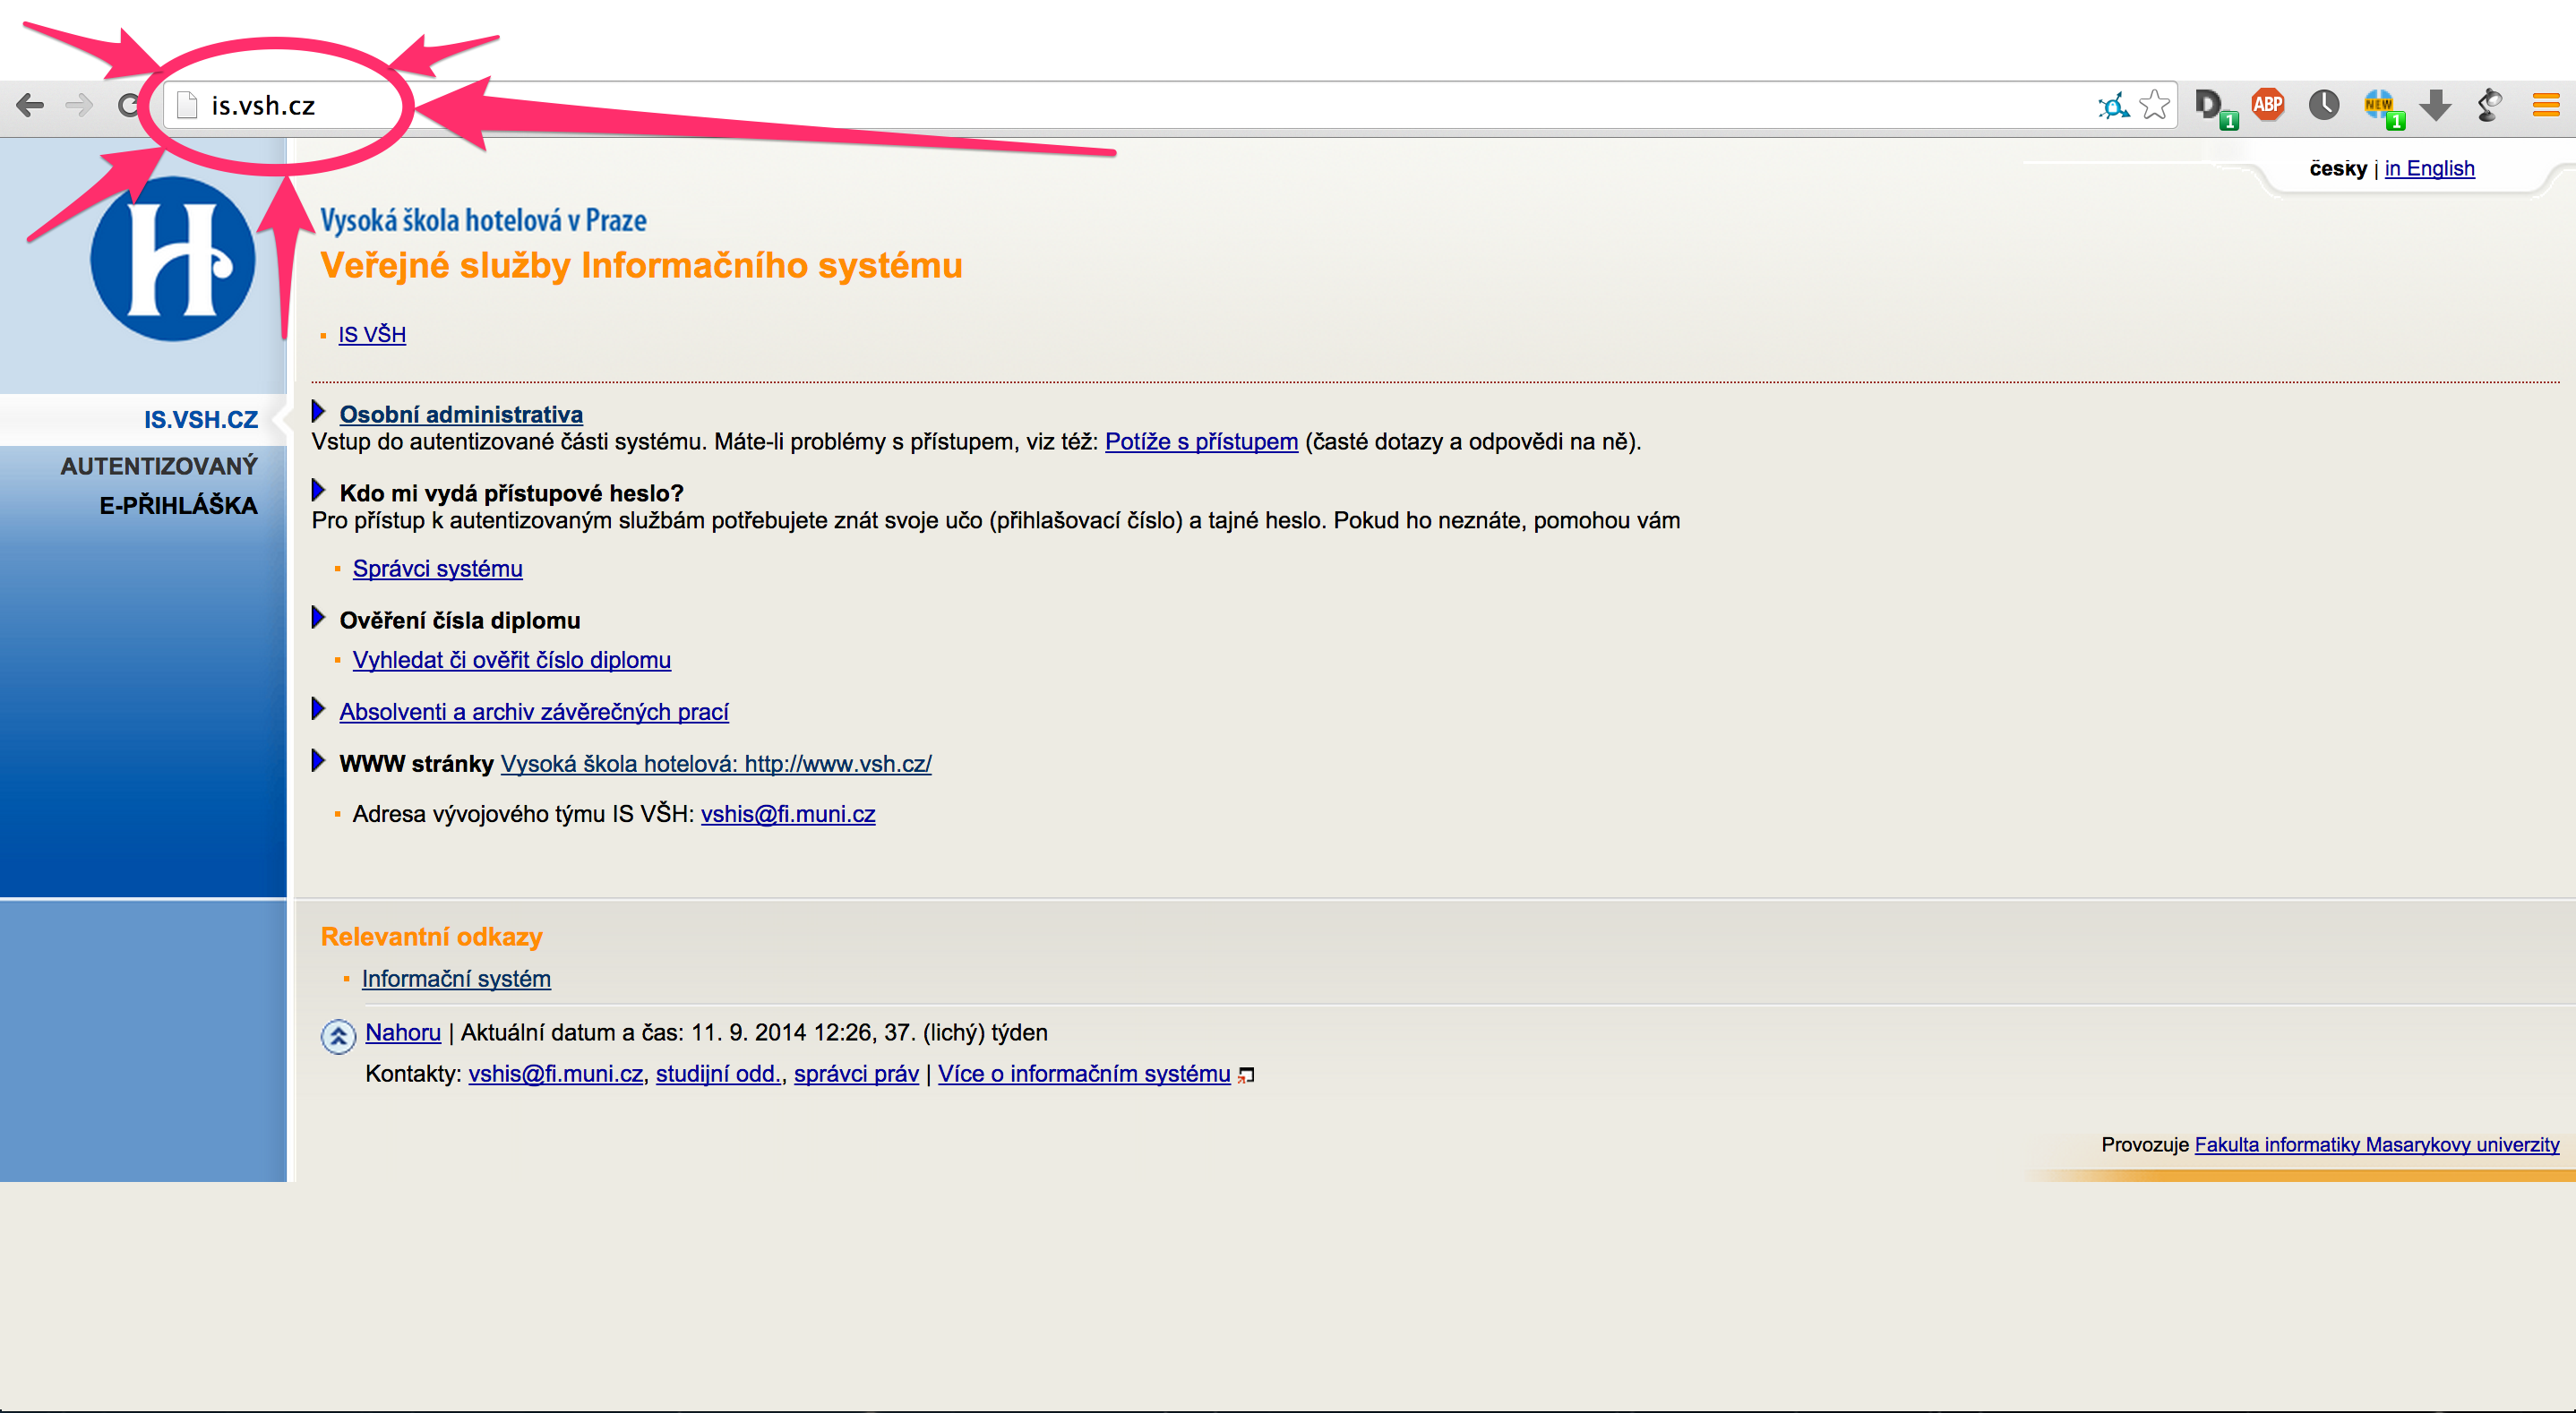
\includegraphics[width=\textwidth]{s01} \\

Nyní klikněte na tlačítko \href{http://is.vsh.cz/auth}{AUTENTIZOVANÝ} \\

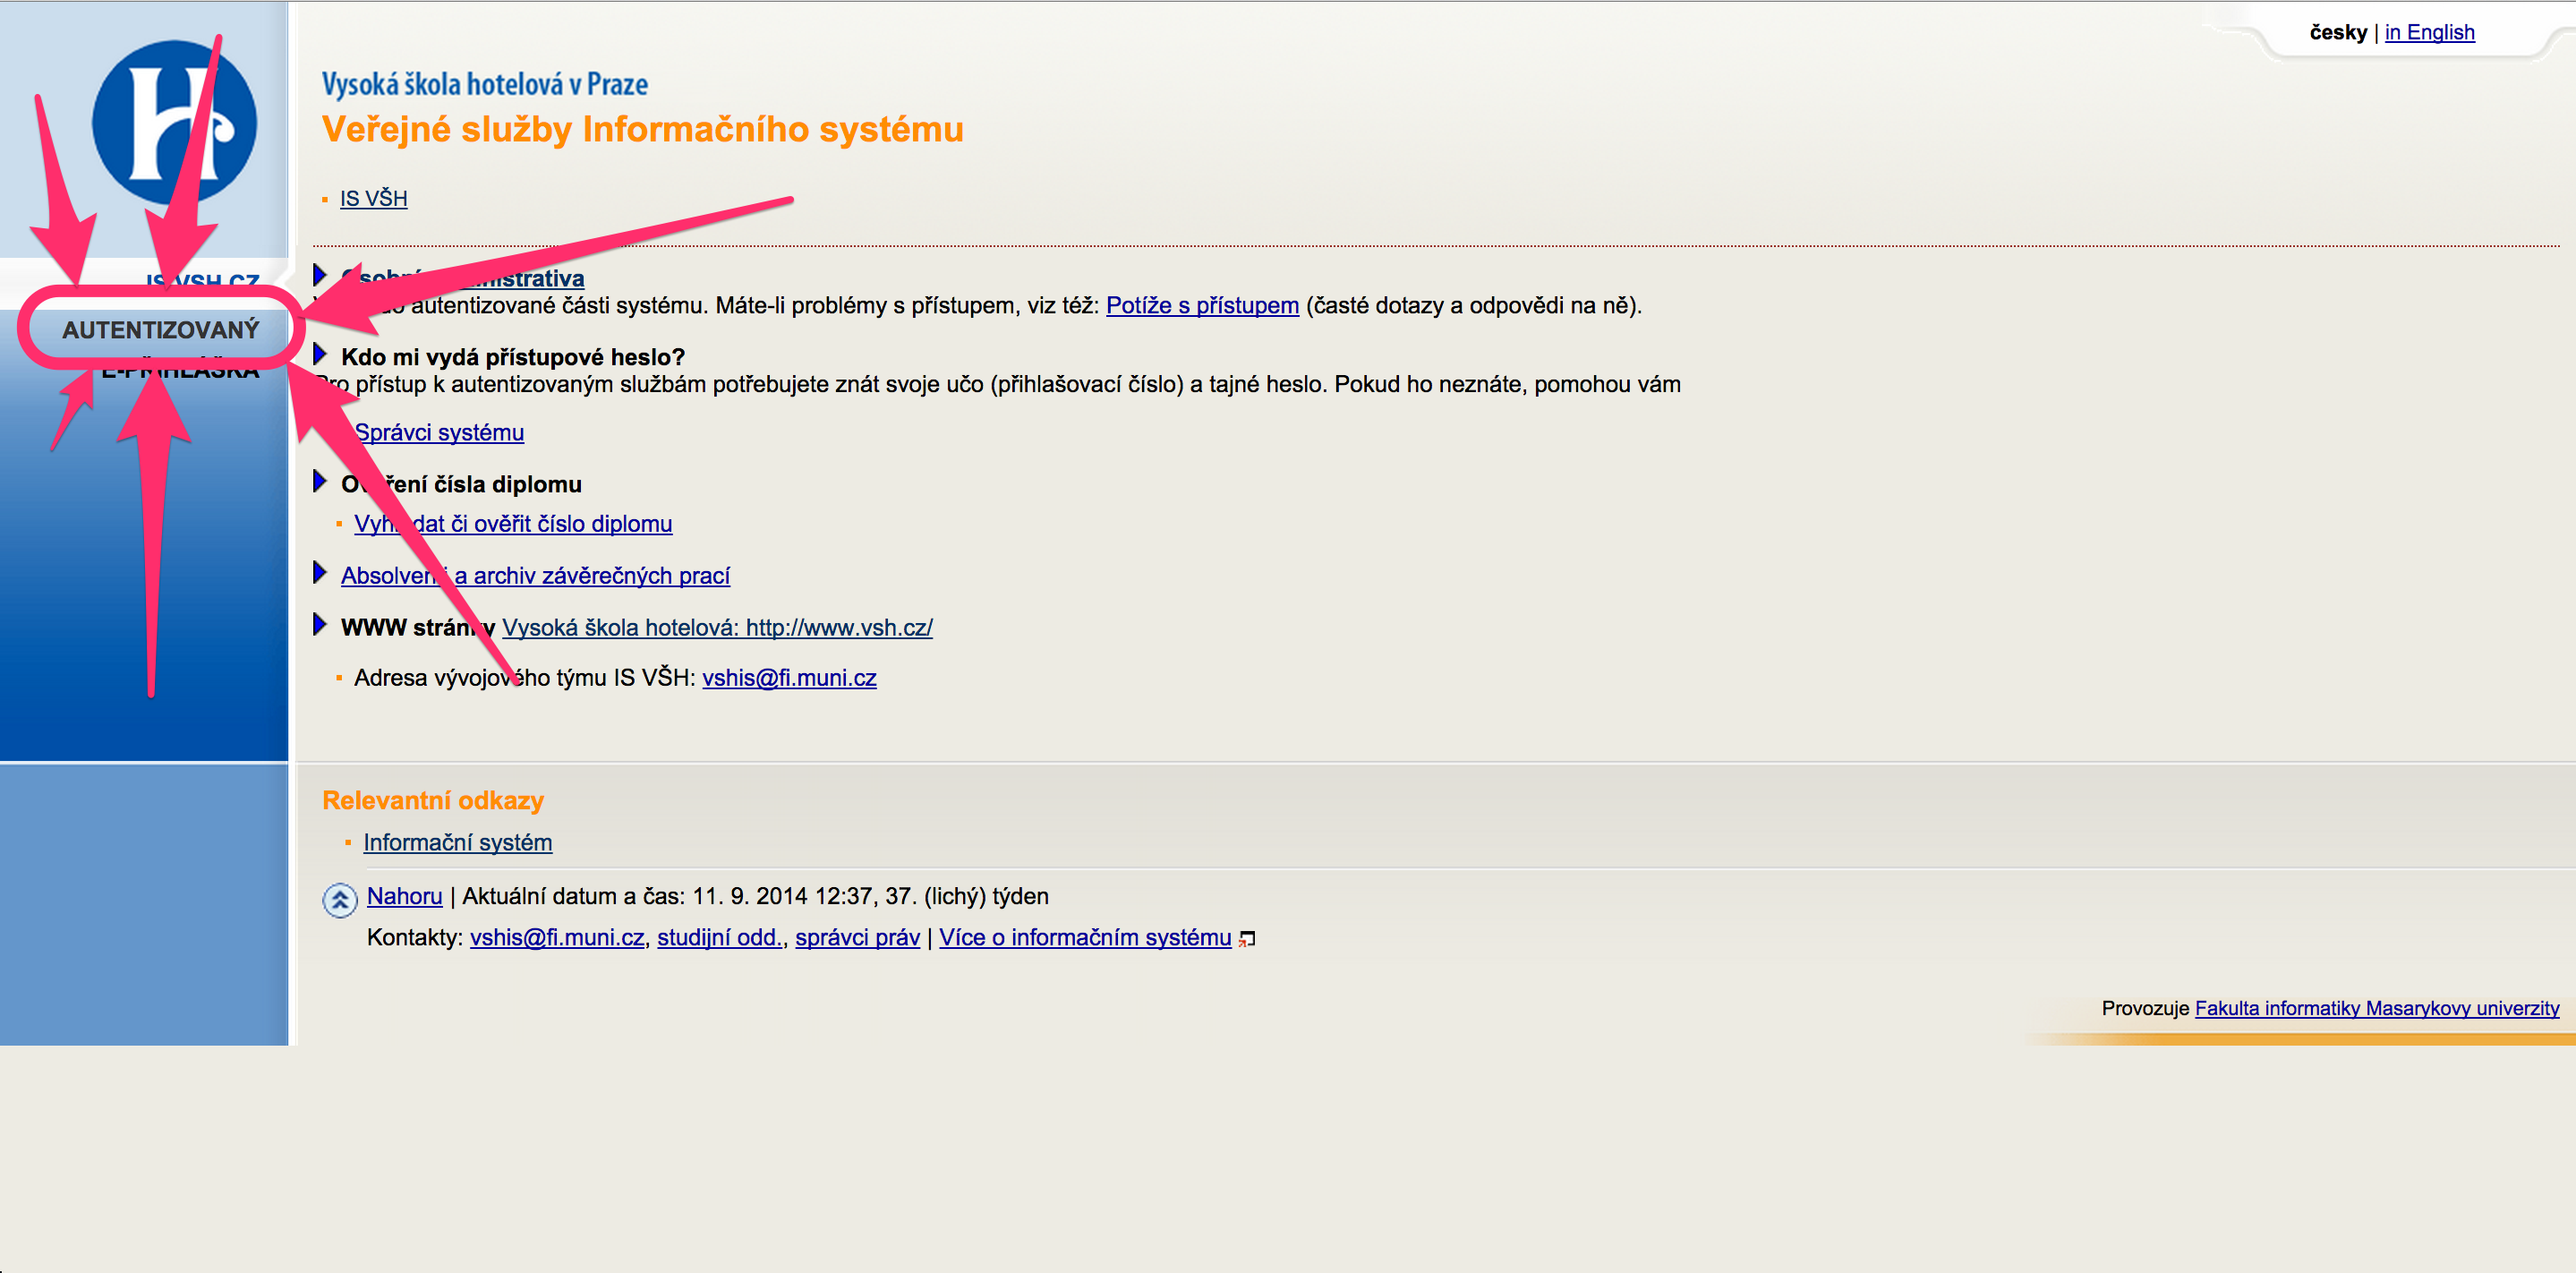
\includegraphics[width=\textwidth]{s02} \\

\newpage

Poté se dostanete na stránku s vaším jménem a heslem. \\

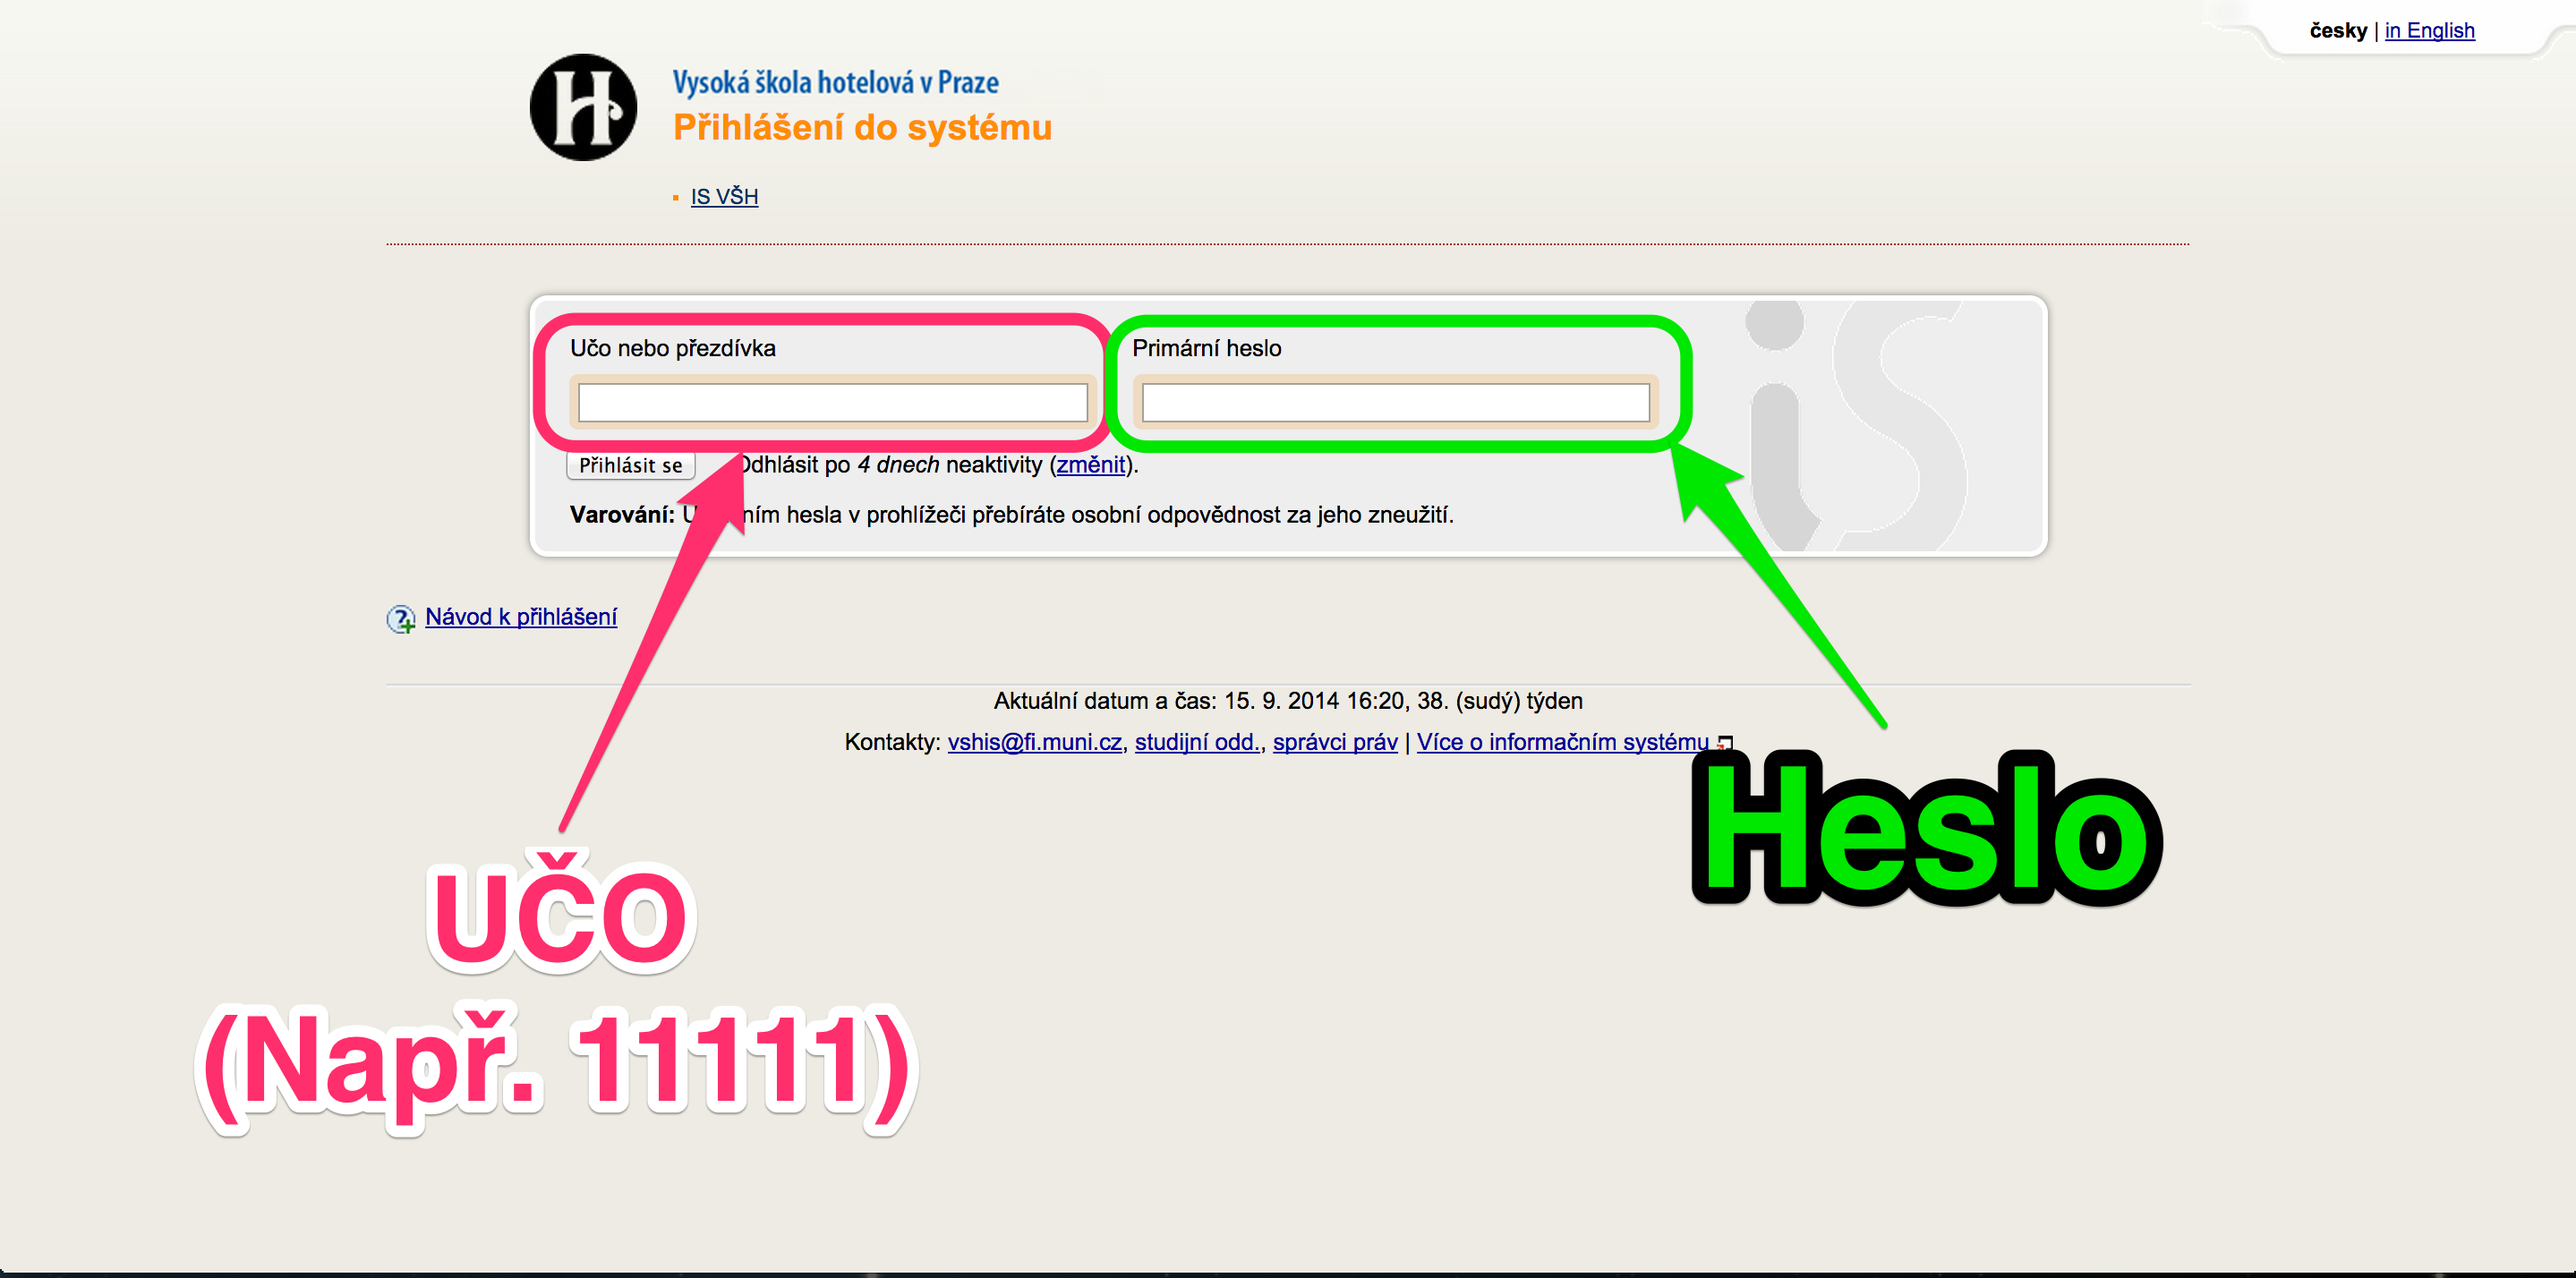
\includegraphics[width=\textwidth]{s03-1} \\

Kde vidíte \textbf{Učo nebo přezdívka} zadejte UČO, v pravém poli zadejte heslo. 
UČO a heslo by mělo být napsáno na papír, který jste museli dostat od studijní referentky.

Pokud všechno proběhlo správně, dostanete se do systému.

\subsection{První pohled}
Tady jsme na hlavní stránce informační systemy VŠH. \\

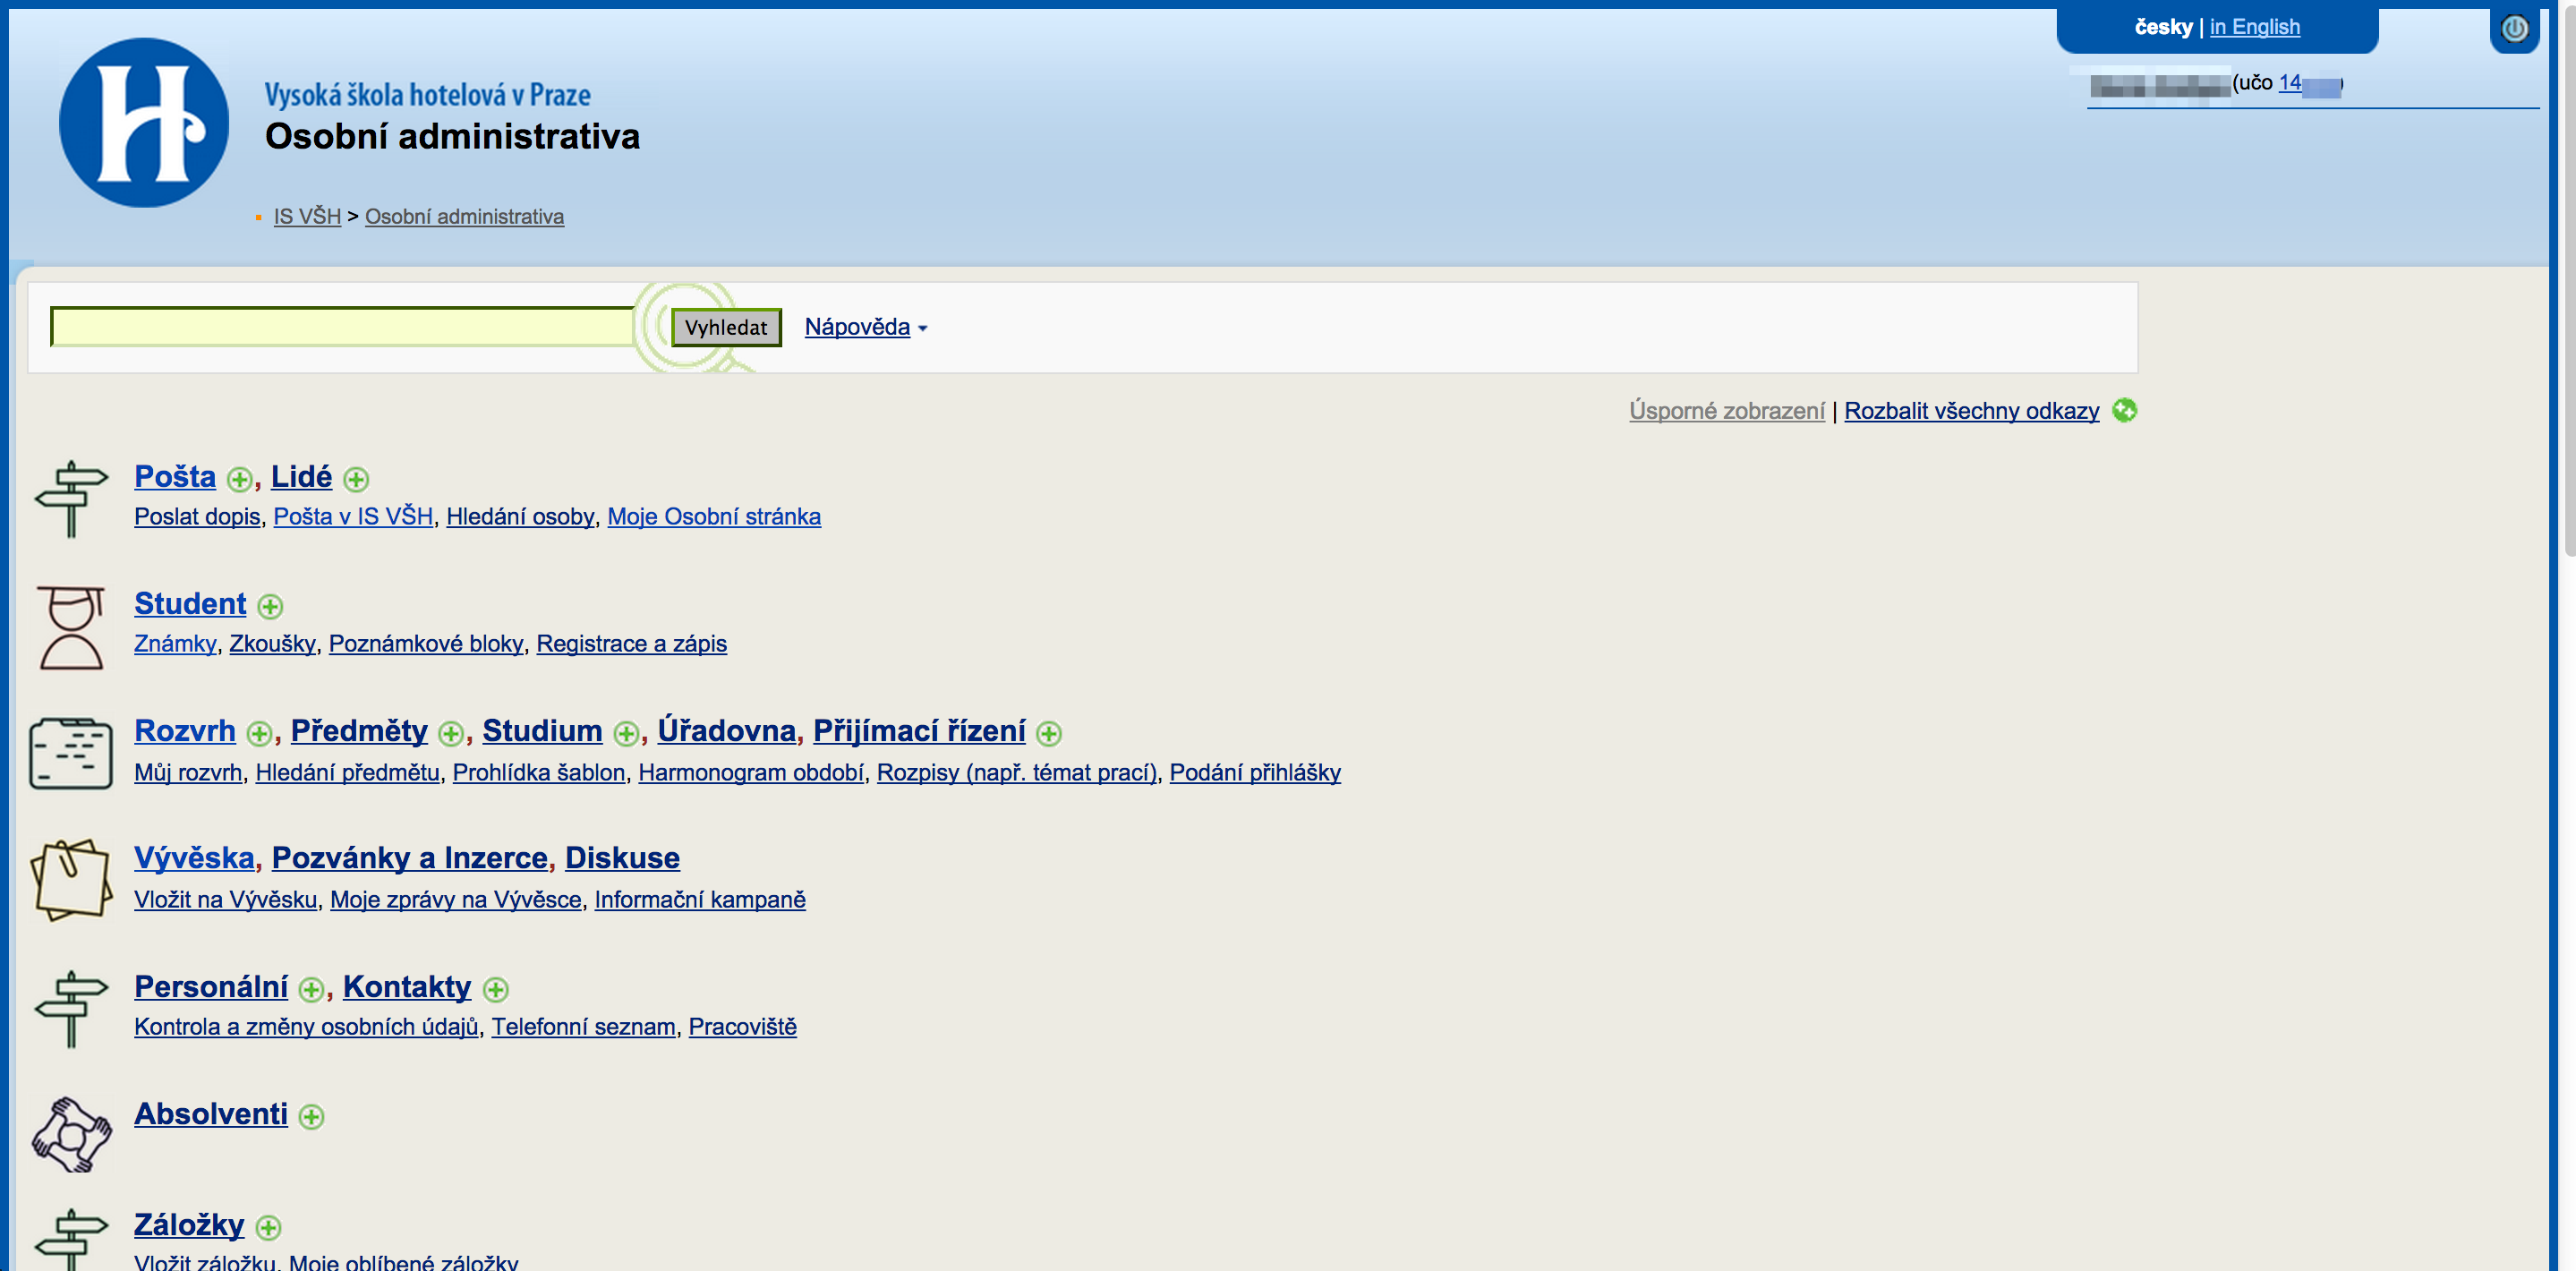
\includegraphics[width=\textwidth]{s04} \\

%Каким же Педро надо было быть, что сделать такую Кончиту?
%Еще и не побоялись написать, что это их работа. Храбрецы!
%Но перейдем к разбору интерфейса. % точнее, к его отсутствию

\newpage
\subsection{Váš profil}

Chcete-li zobrazit svůj profil, klepněte na vašem čislu UČO v pravém horním rohu. \\

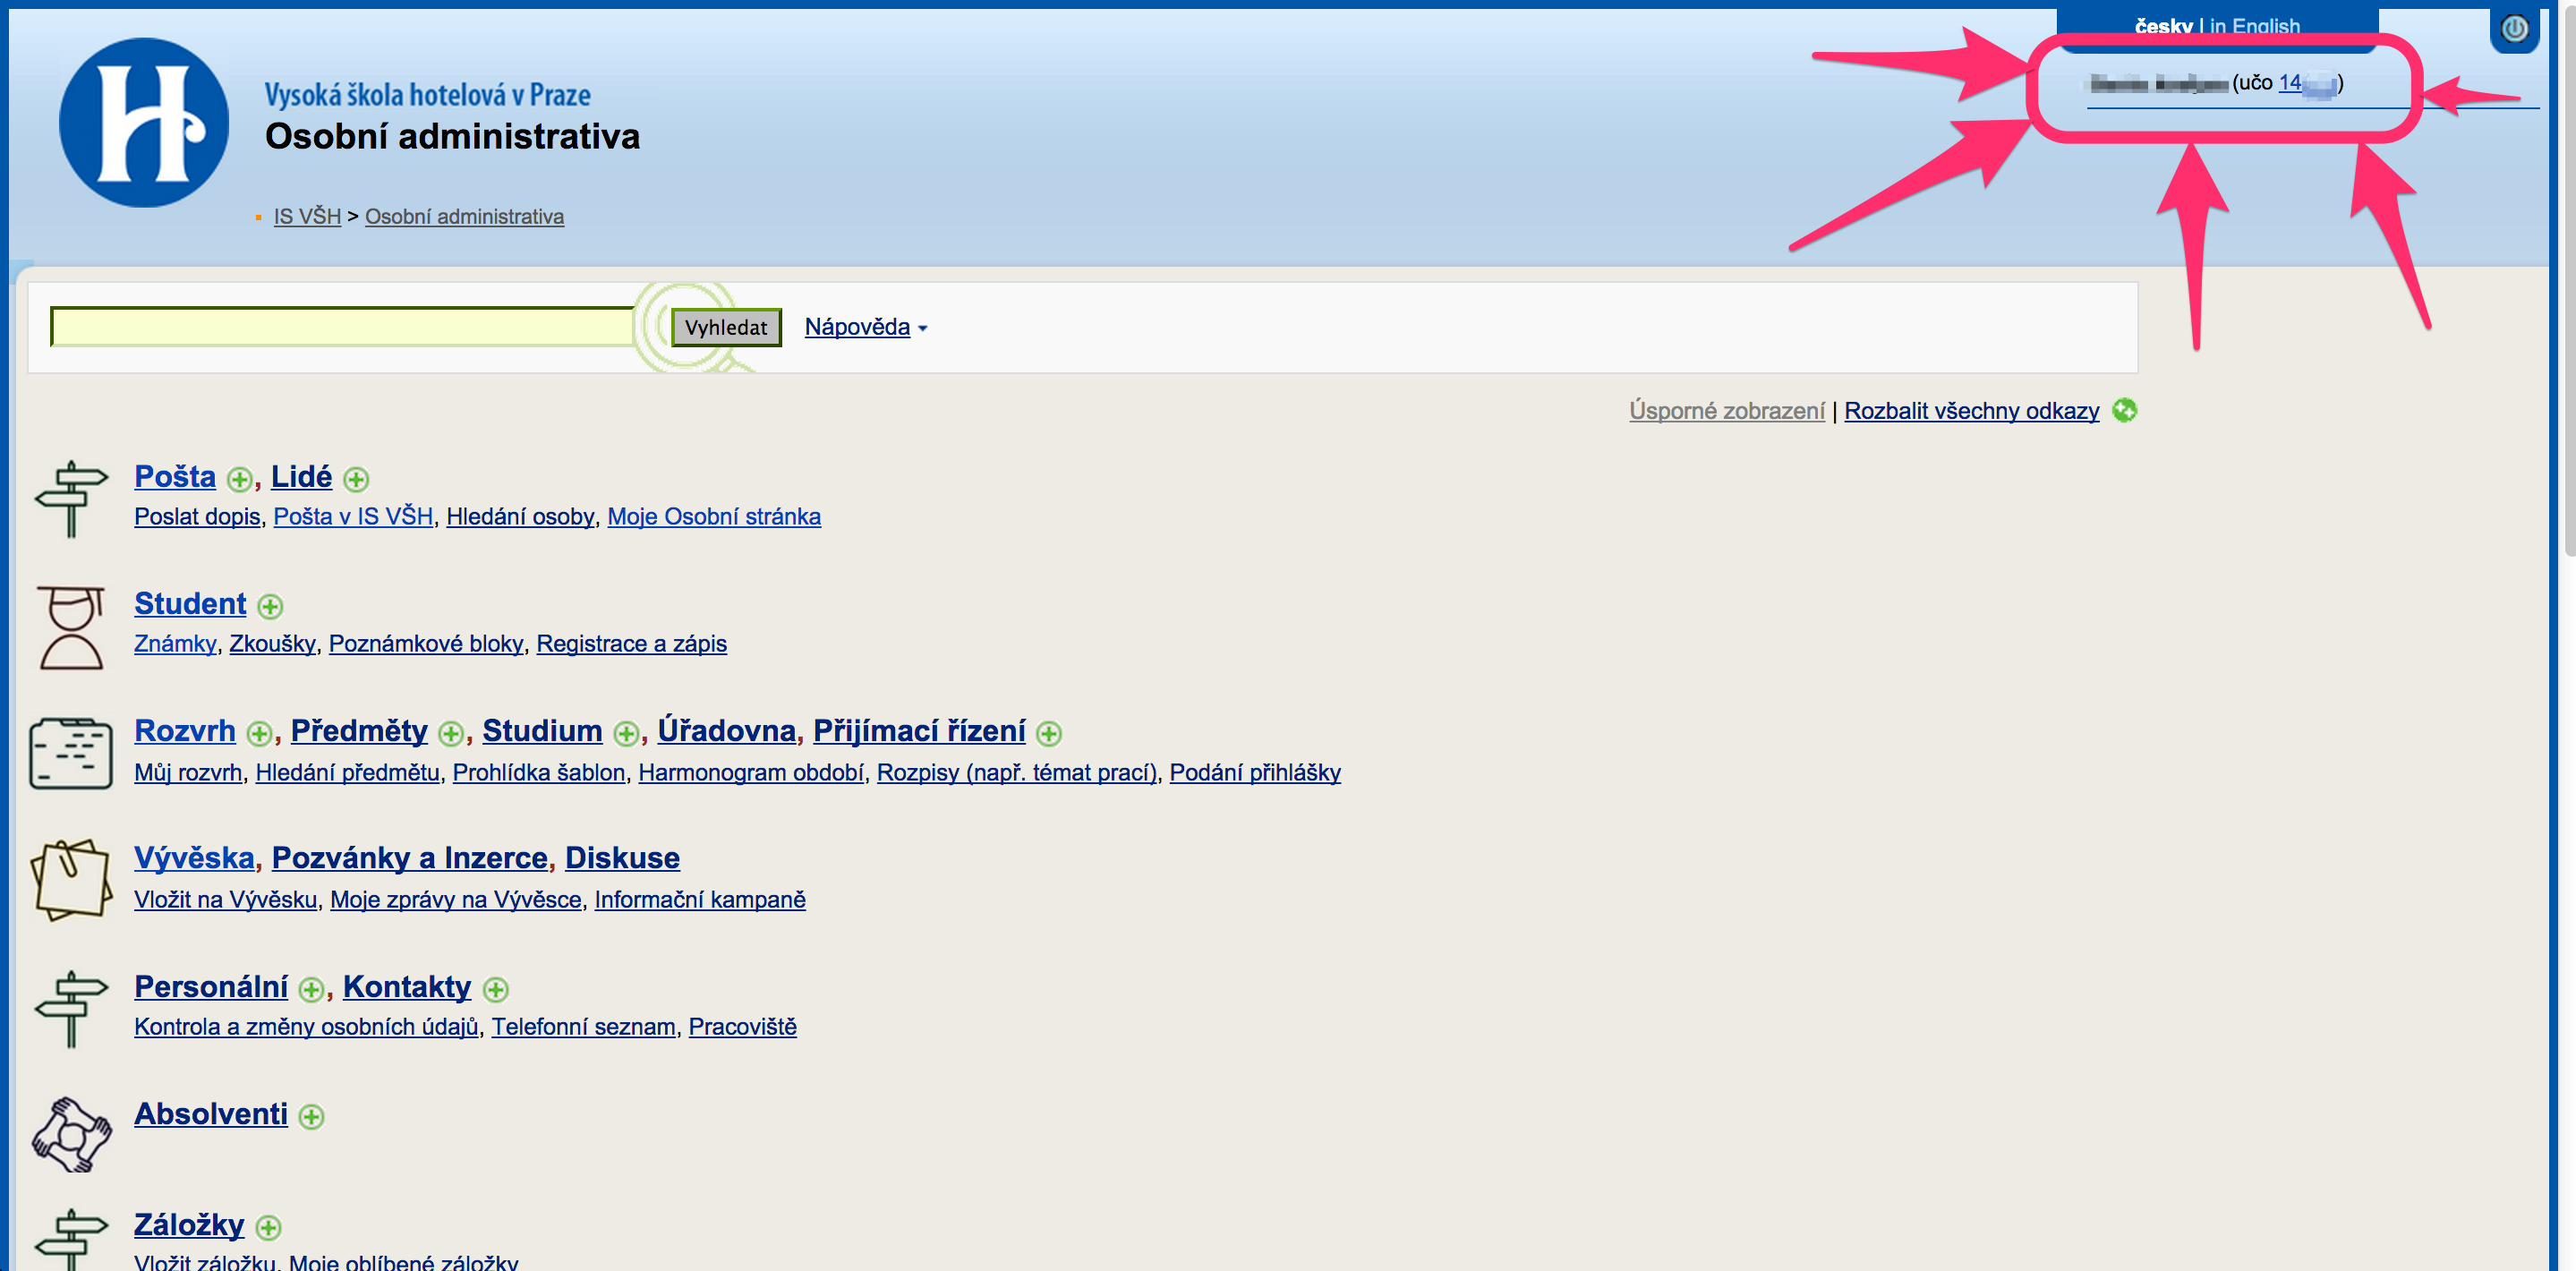
\includegraphics[width=\textwidth]{s05} \\

Ve vašem profilu naleznete svůj obrázek, vaše jméno a UČO, oddělení, obor a skupinu. \\

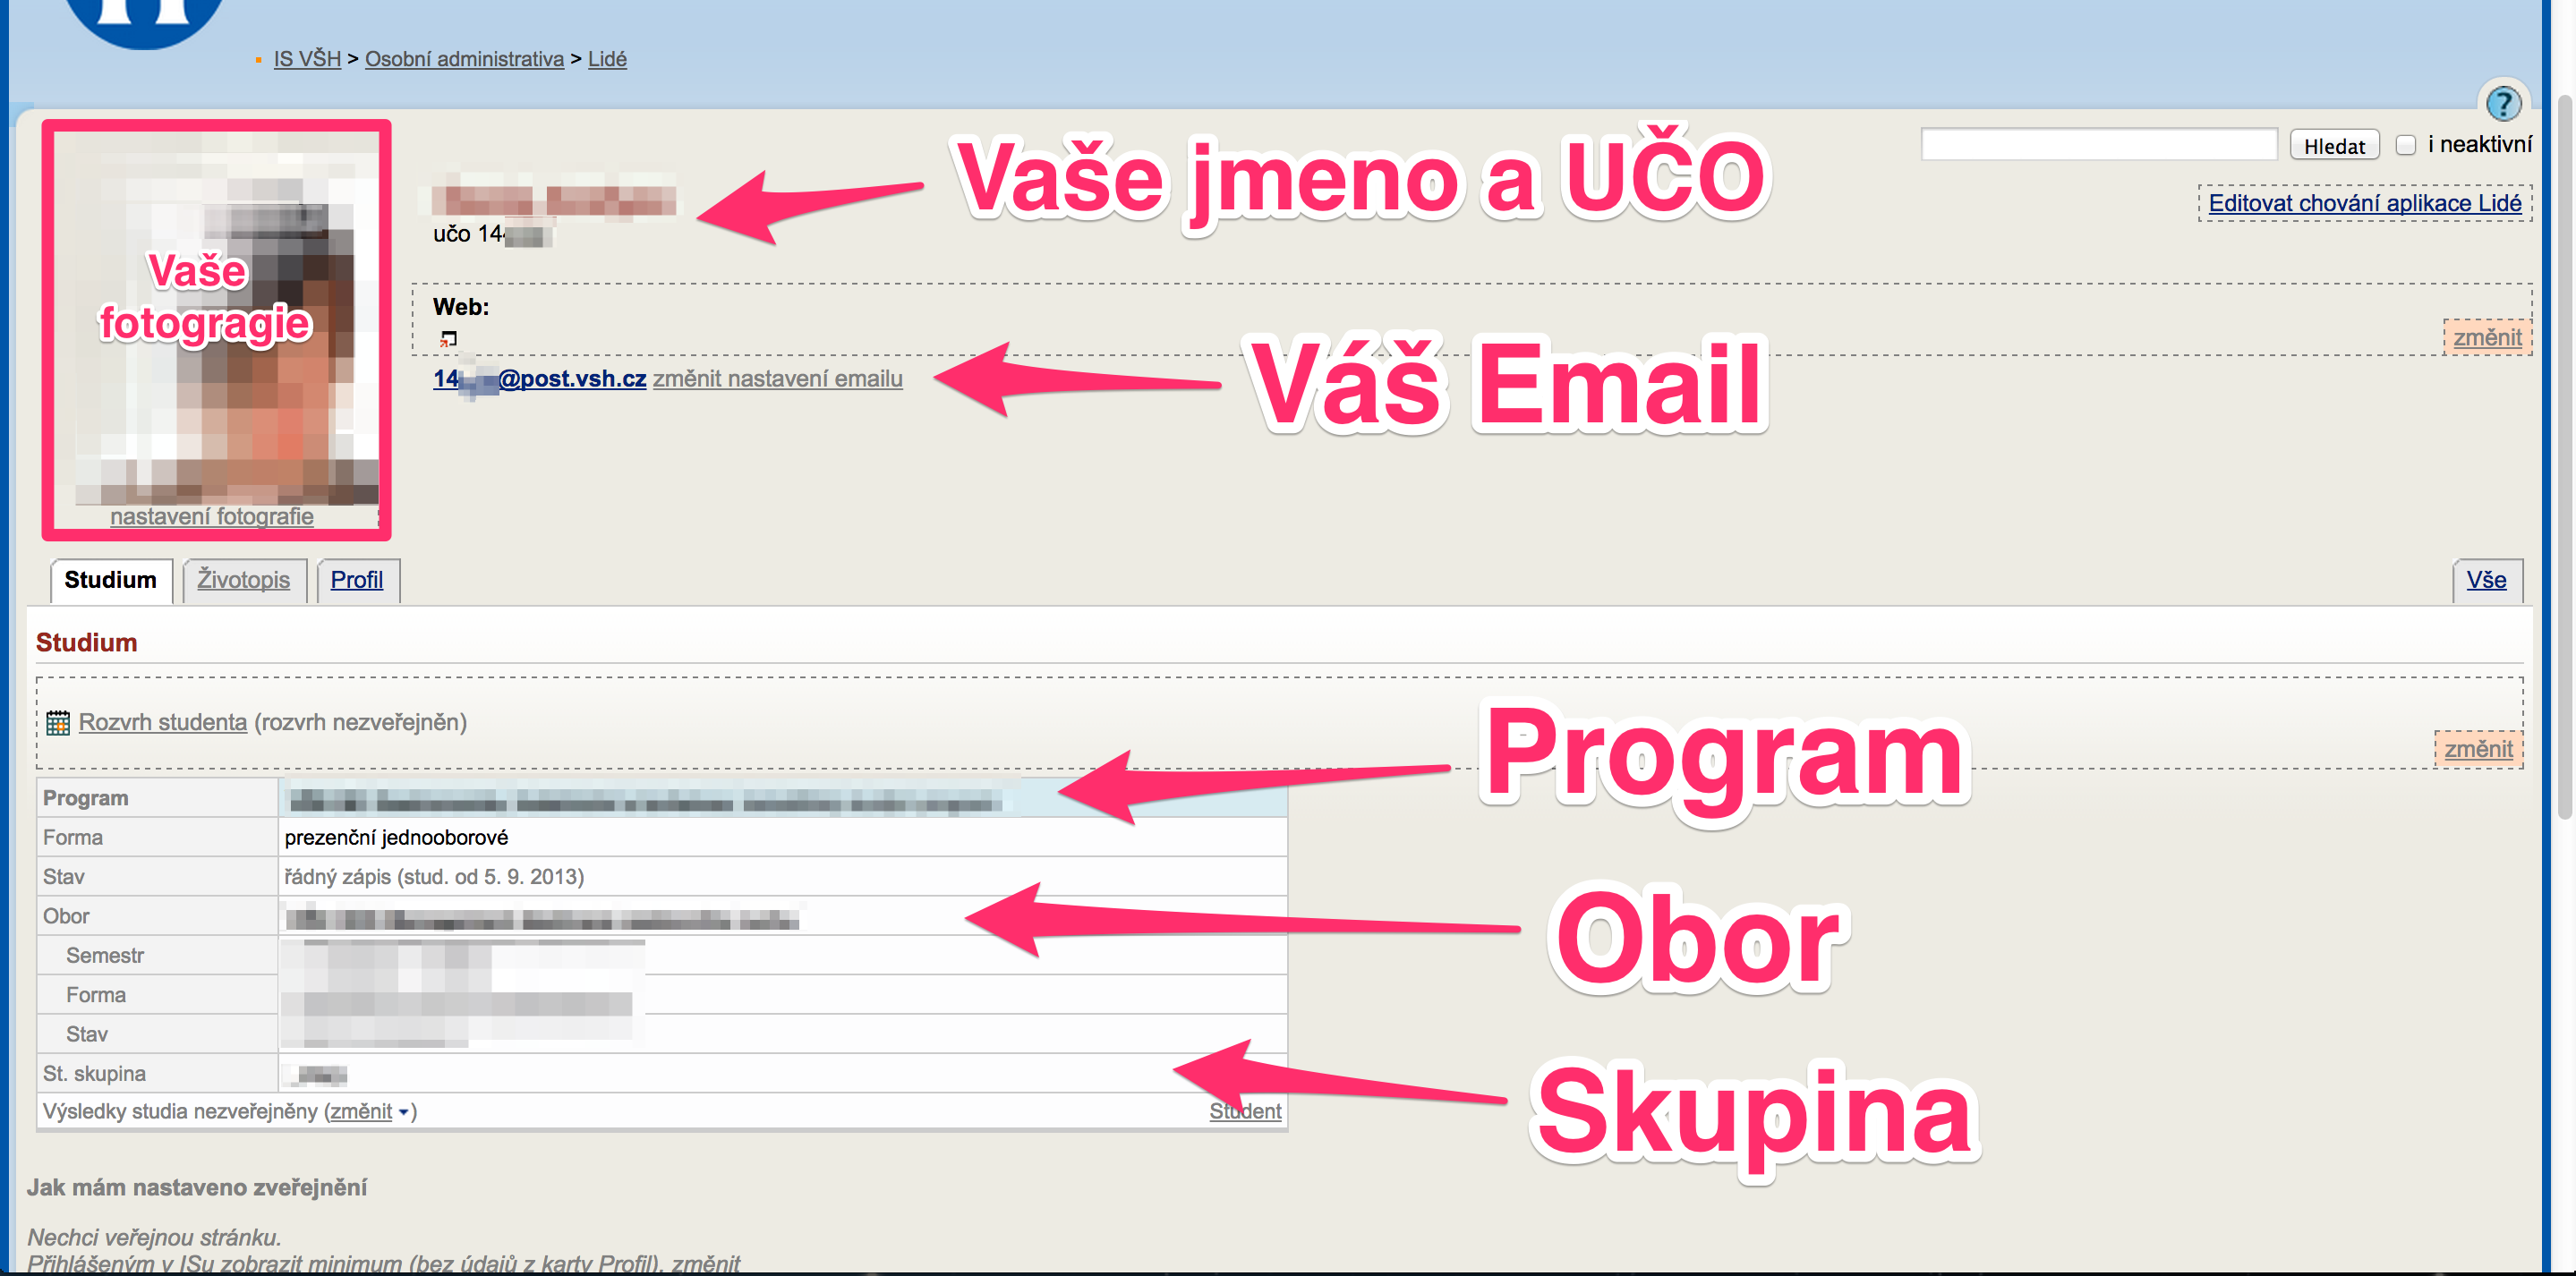
\includegraphics[width=\textwidth]{s06-1} \\

\newpage
Pro návrat do hlavního menu, stačí kliknout na logo školy, 
nebo klikněte na odkaz \textbf{IS VŠH} pod ním. \\

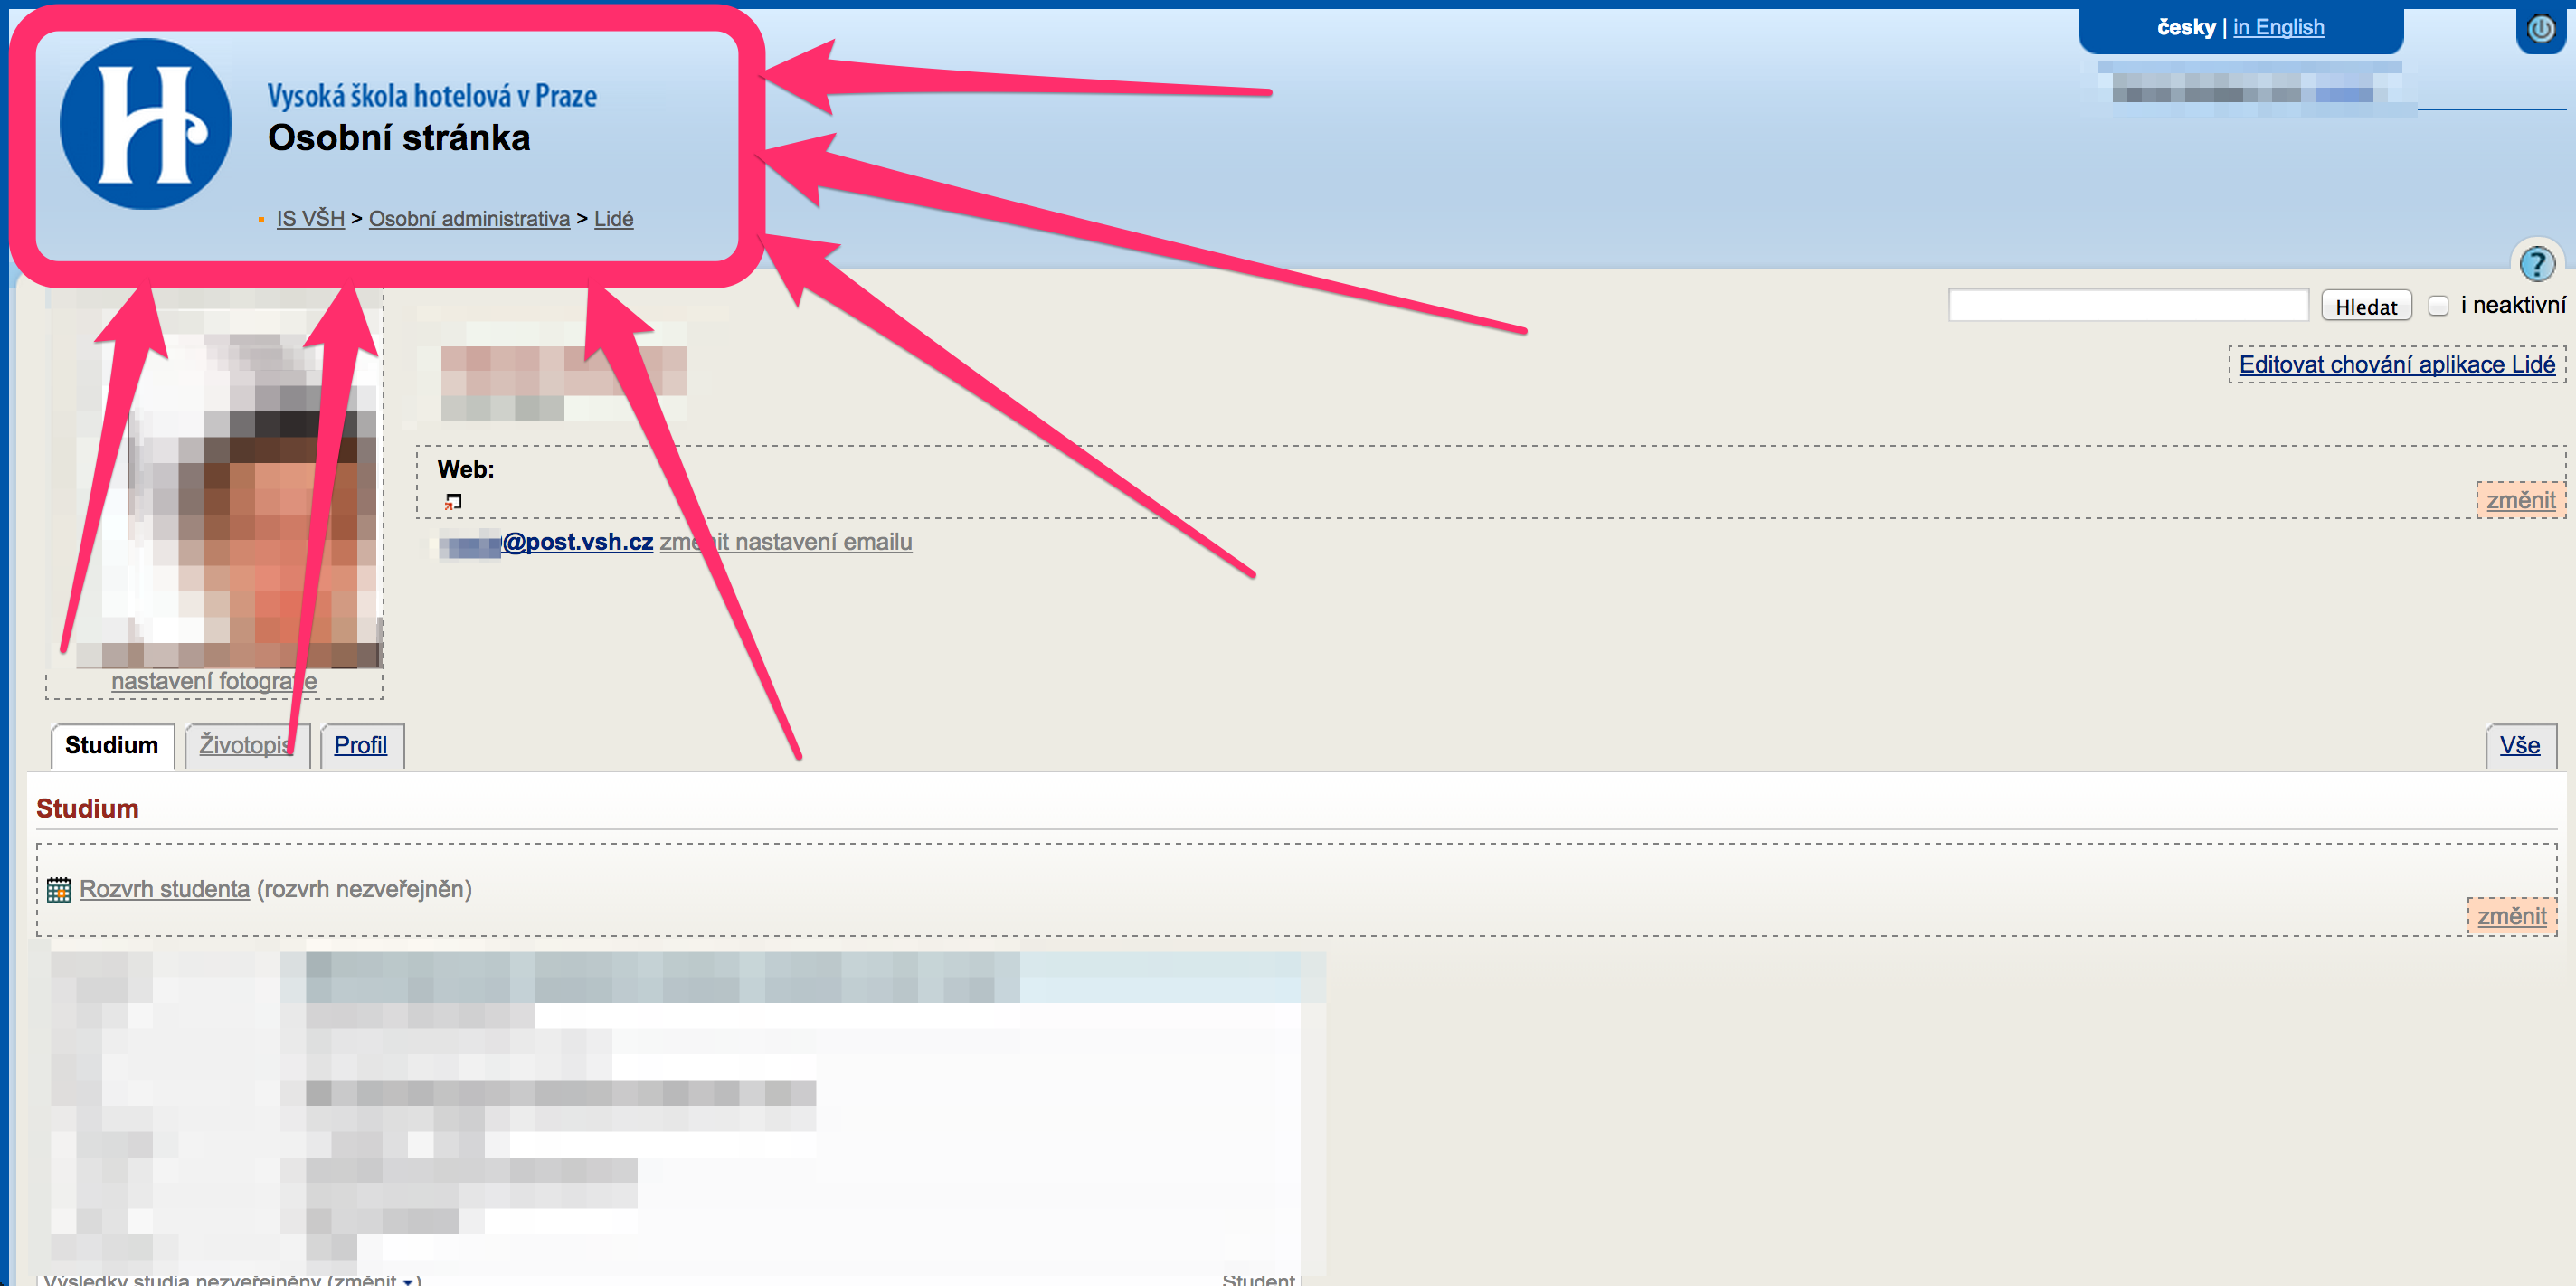
\includegraphics[width=\textwidth]{s07} \\

Jsme zpátky na hlavní stránce! \\

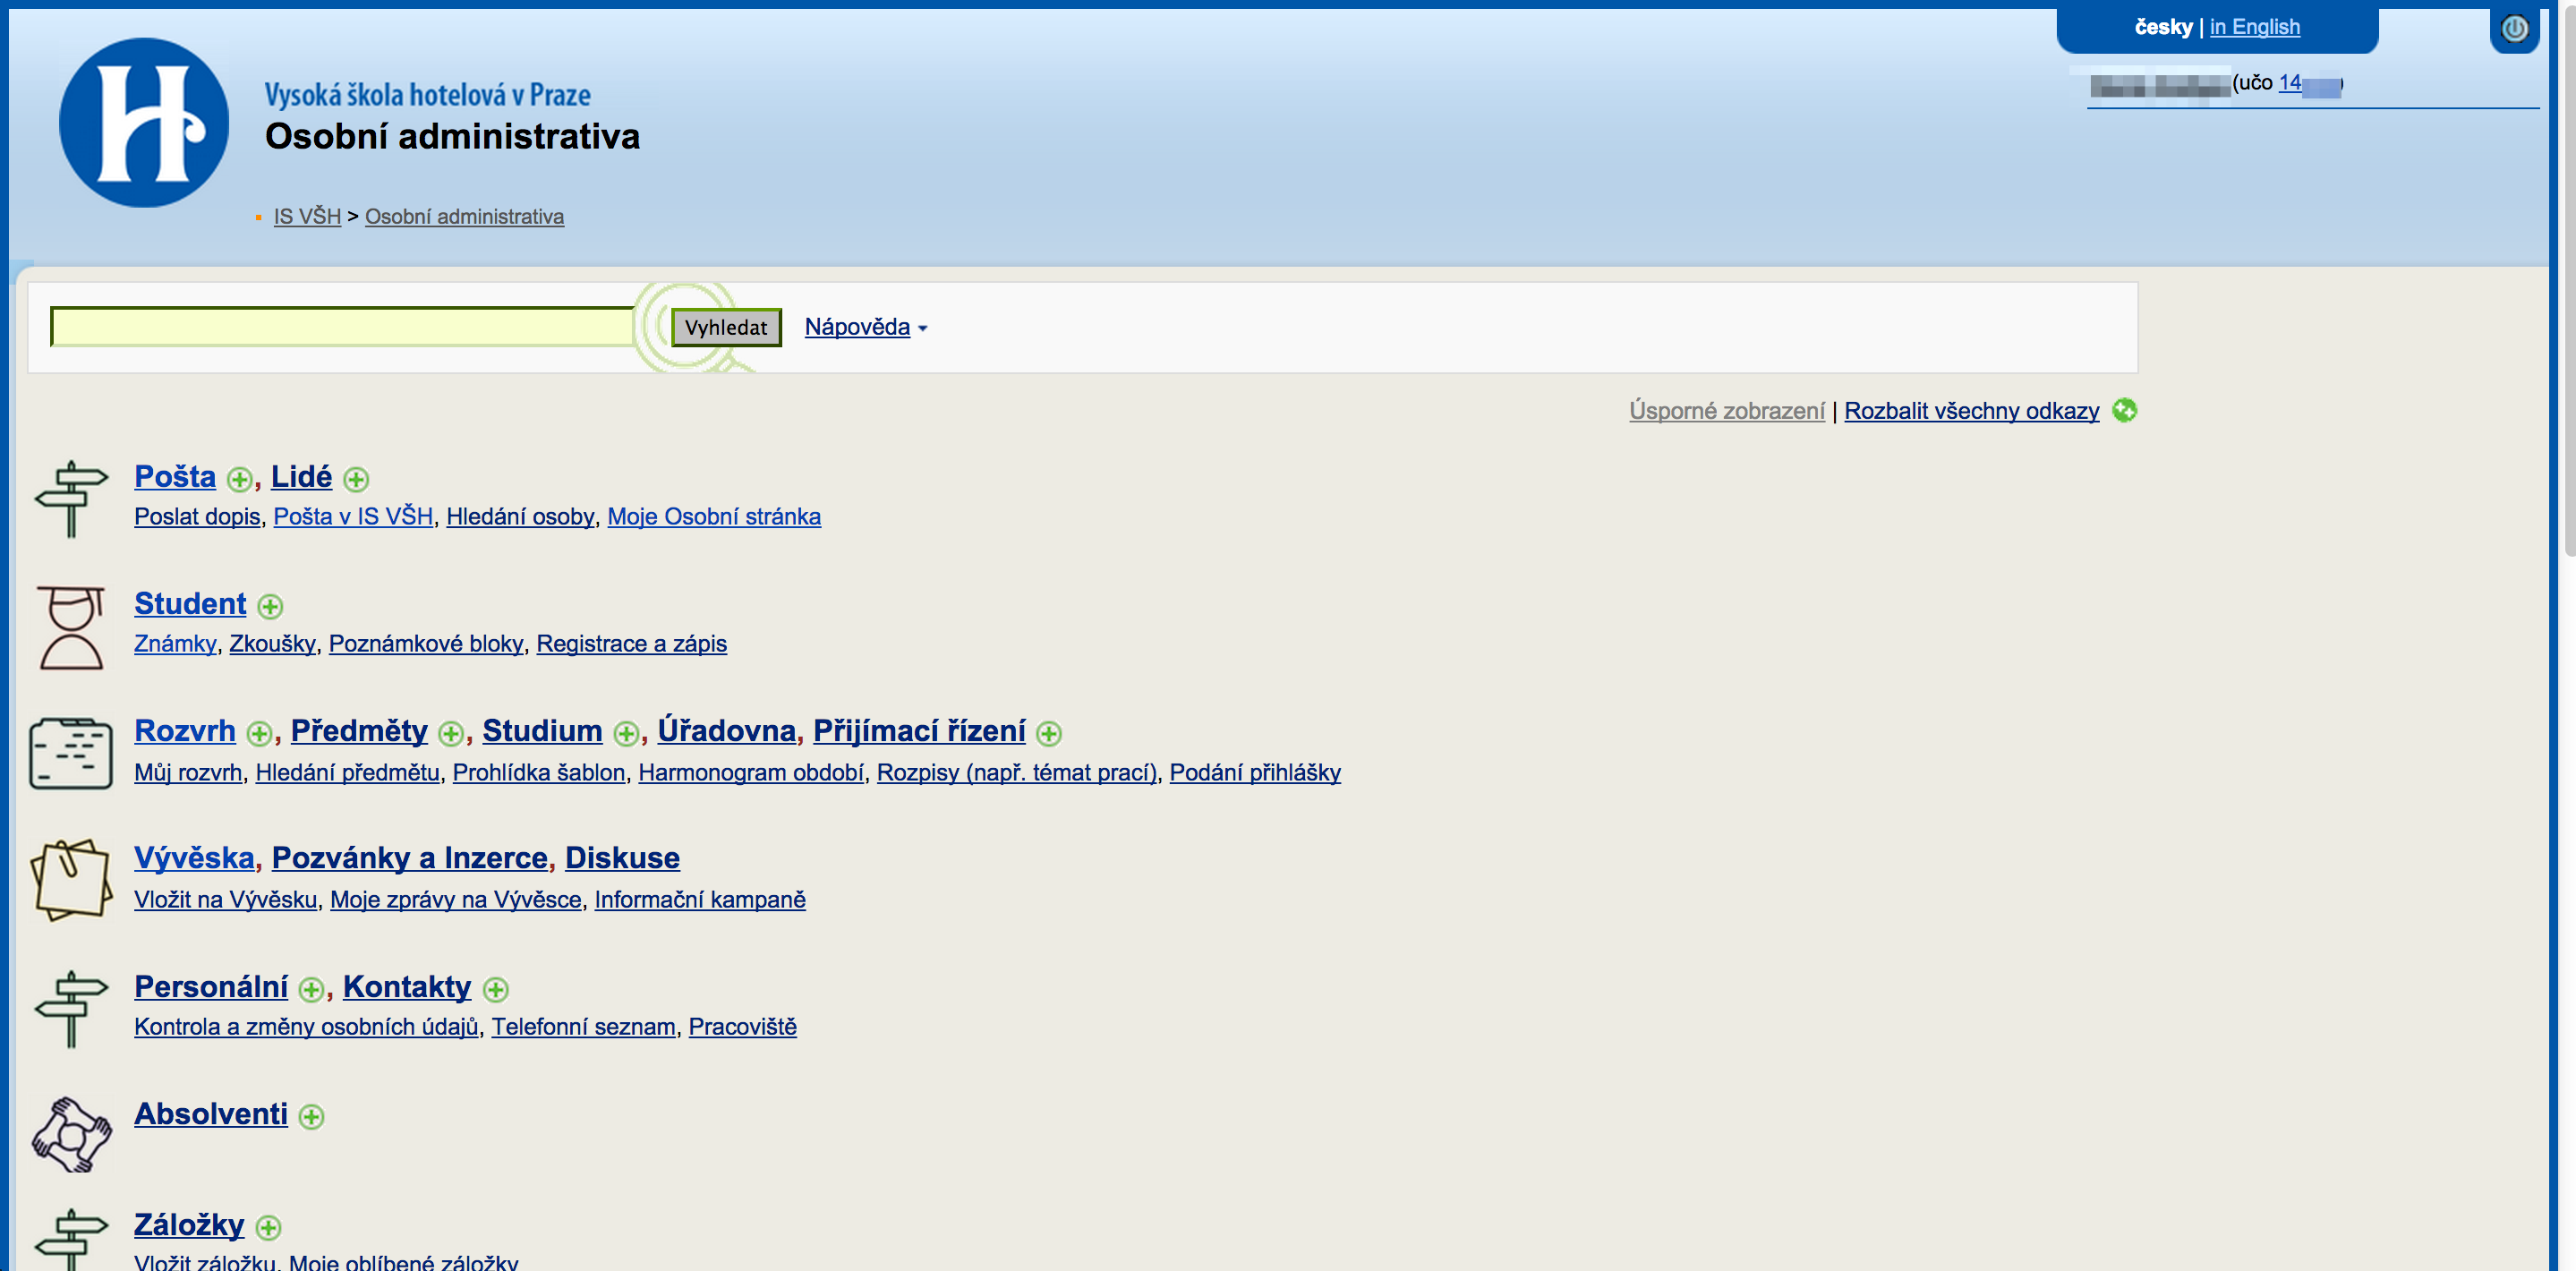
\includegraphics[width=\textwidth]{s04} \\

\newpage

\section{Vaše pošta}
Tak vypadá pošta. Tady se budou dostávat všechné důležité
informace týkající vašeho studia. 
Radím vám, abyste často kontrolovali svou poštu. \\

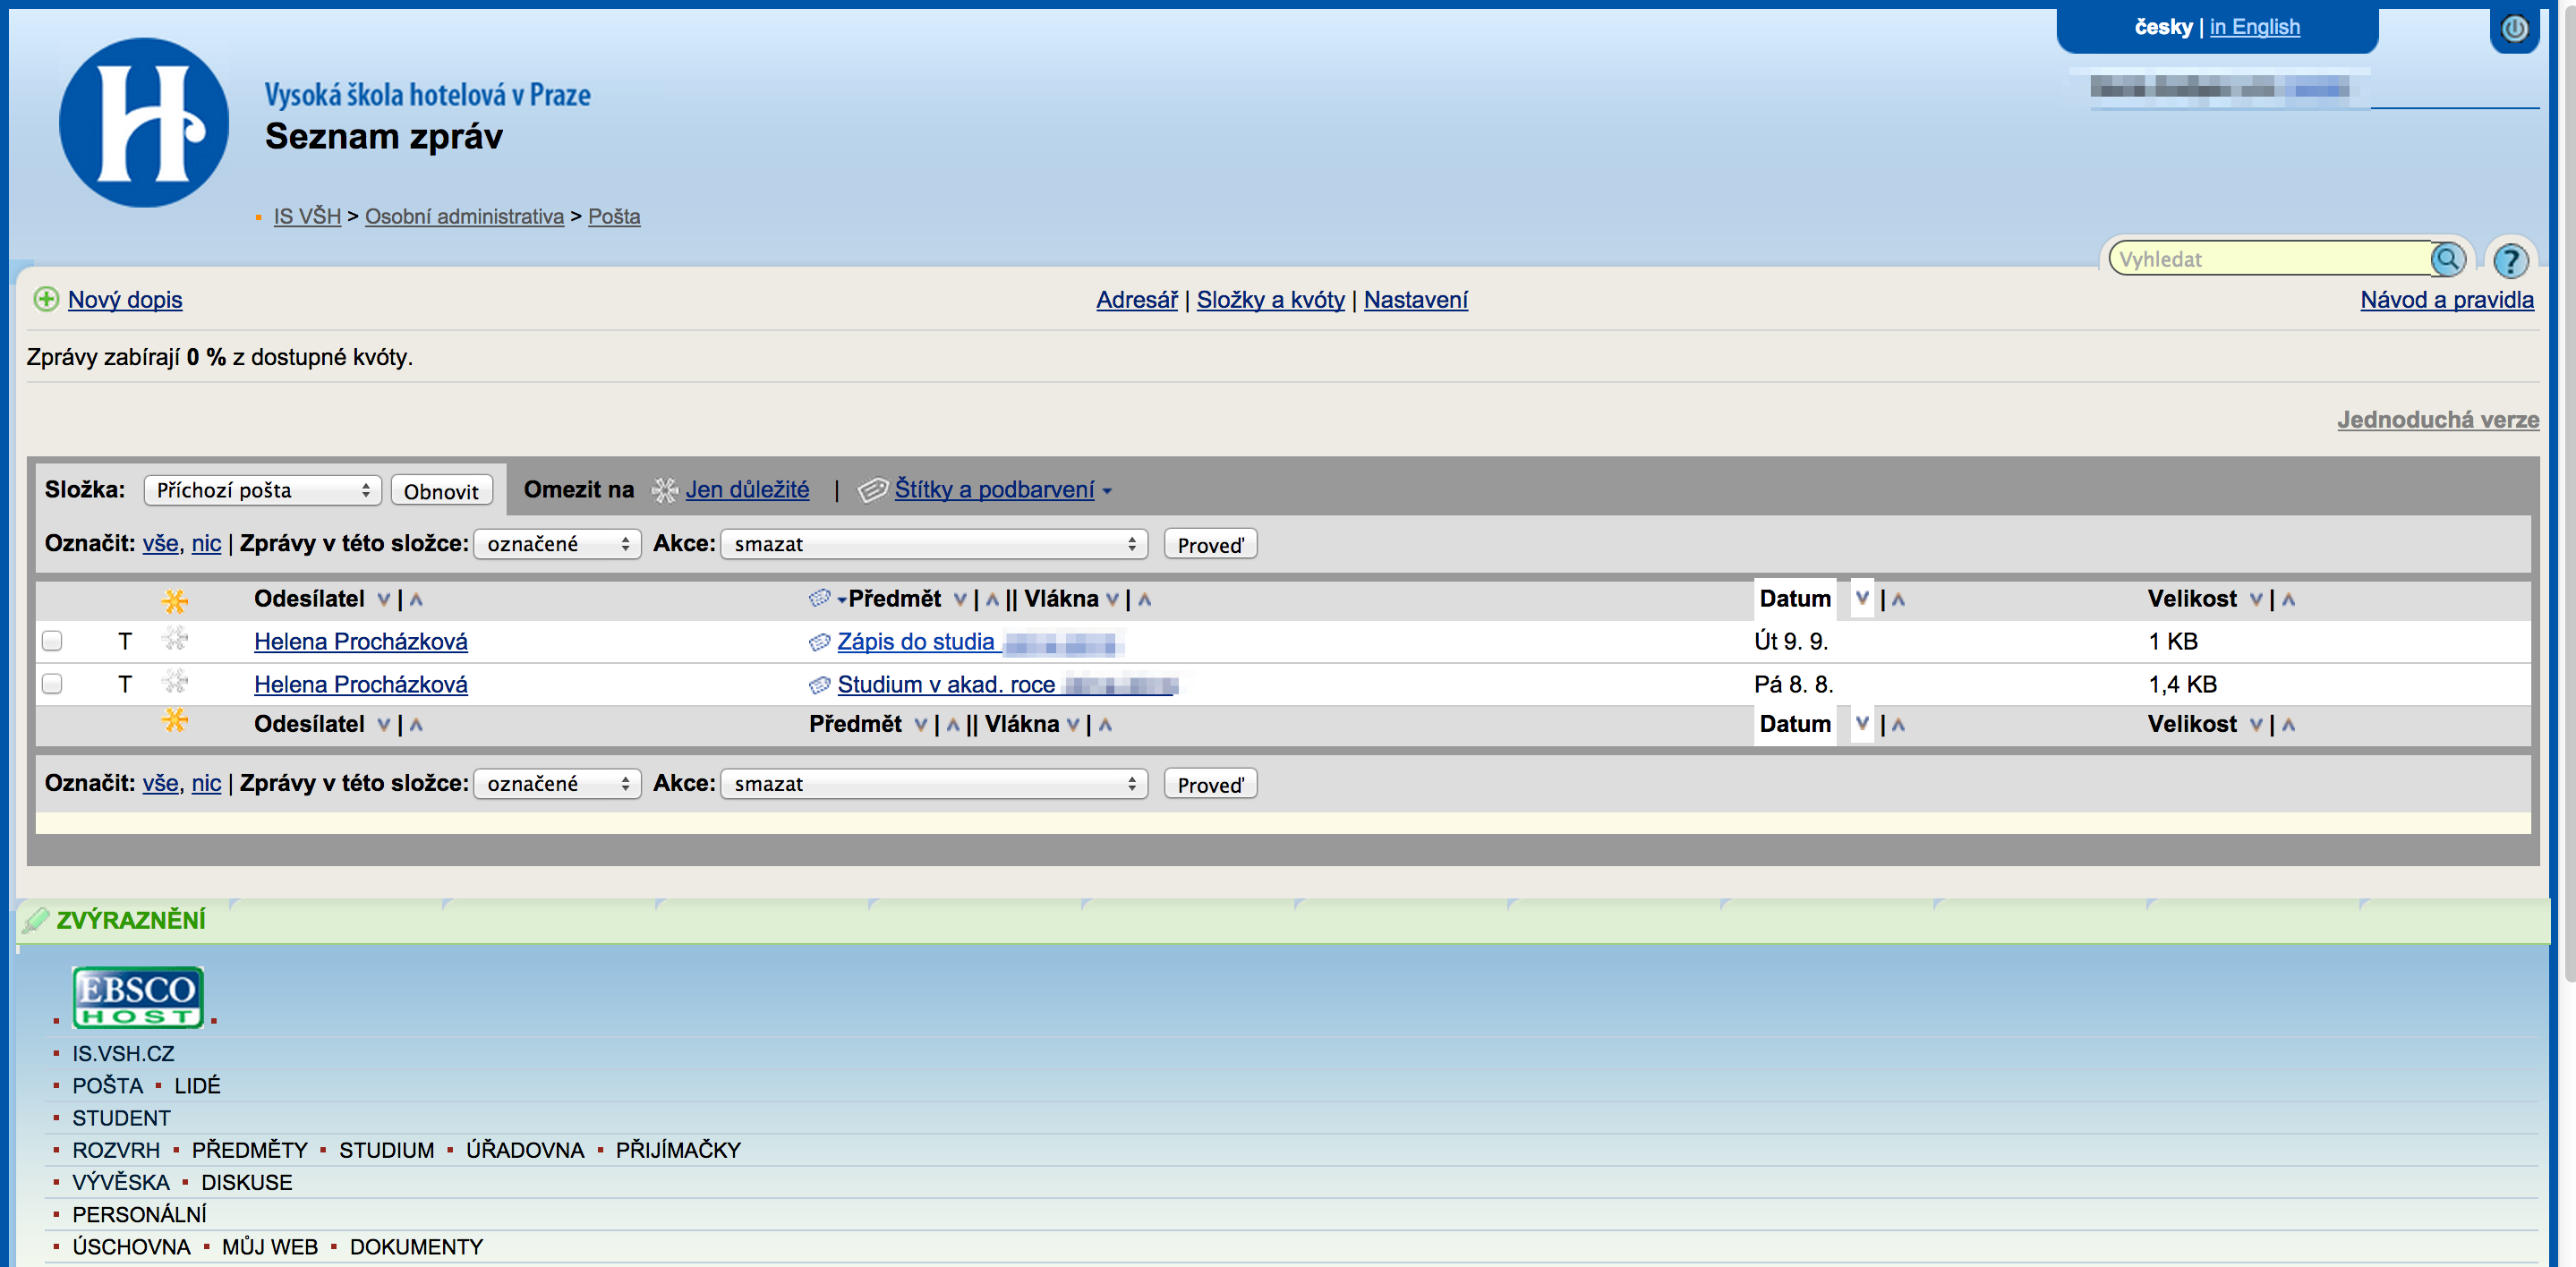
\includegraphics[width=\textwidth]{s08}

\subsection{Napsat dopis}

Chcete-li napsat novou zprávu, stačí kliknout na odkaz \textbf{Nový dopis} nahoře vlevo. \\

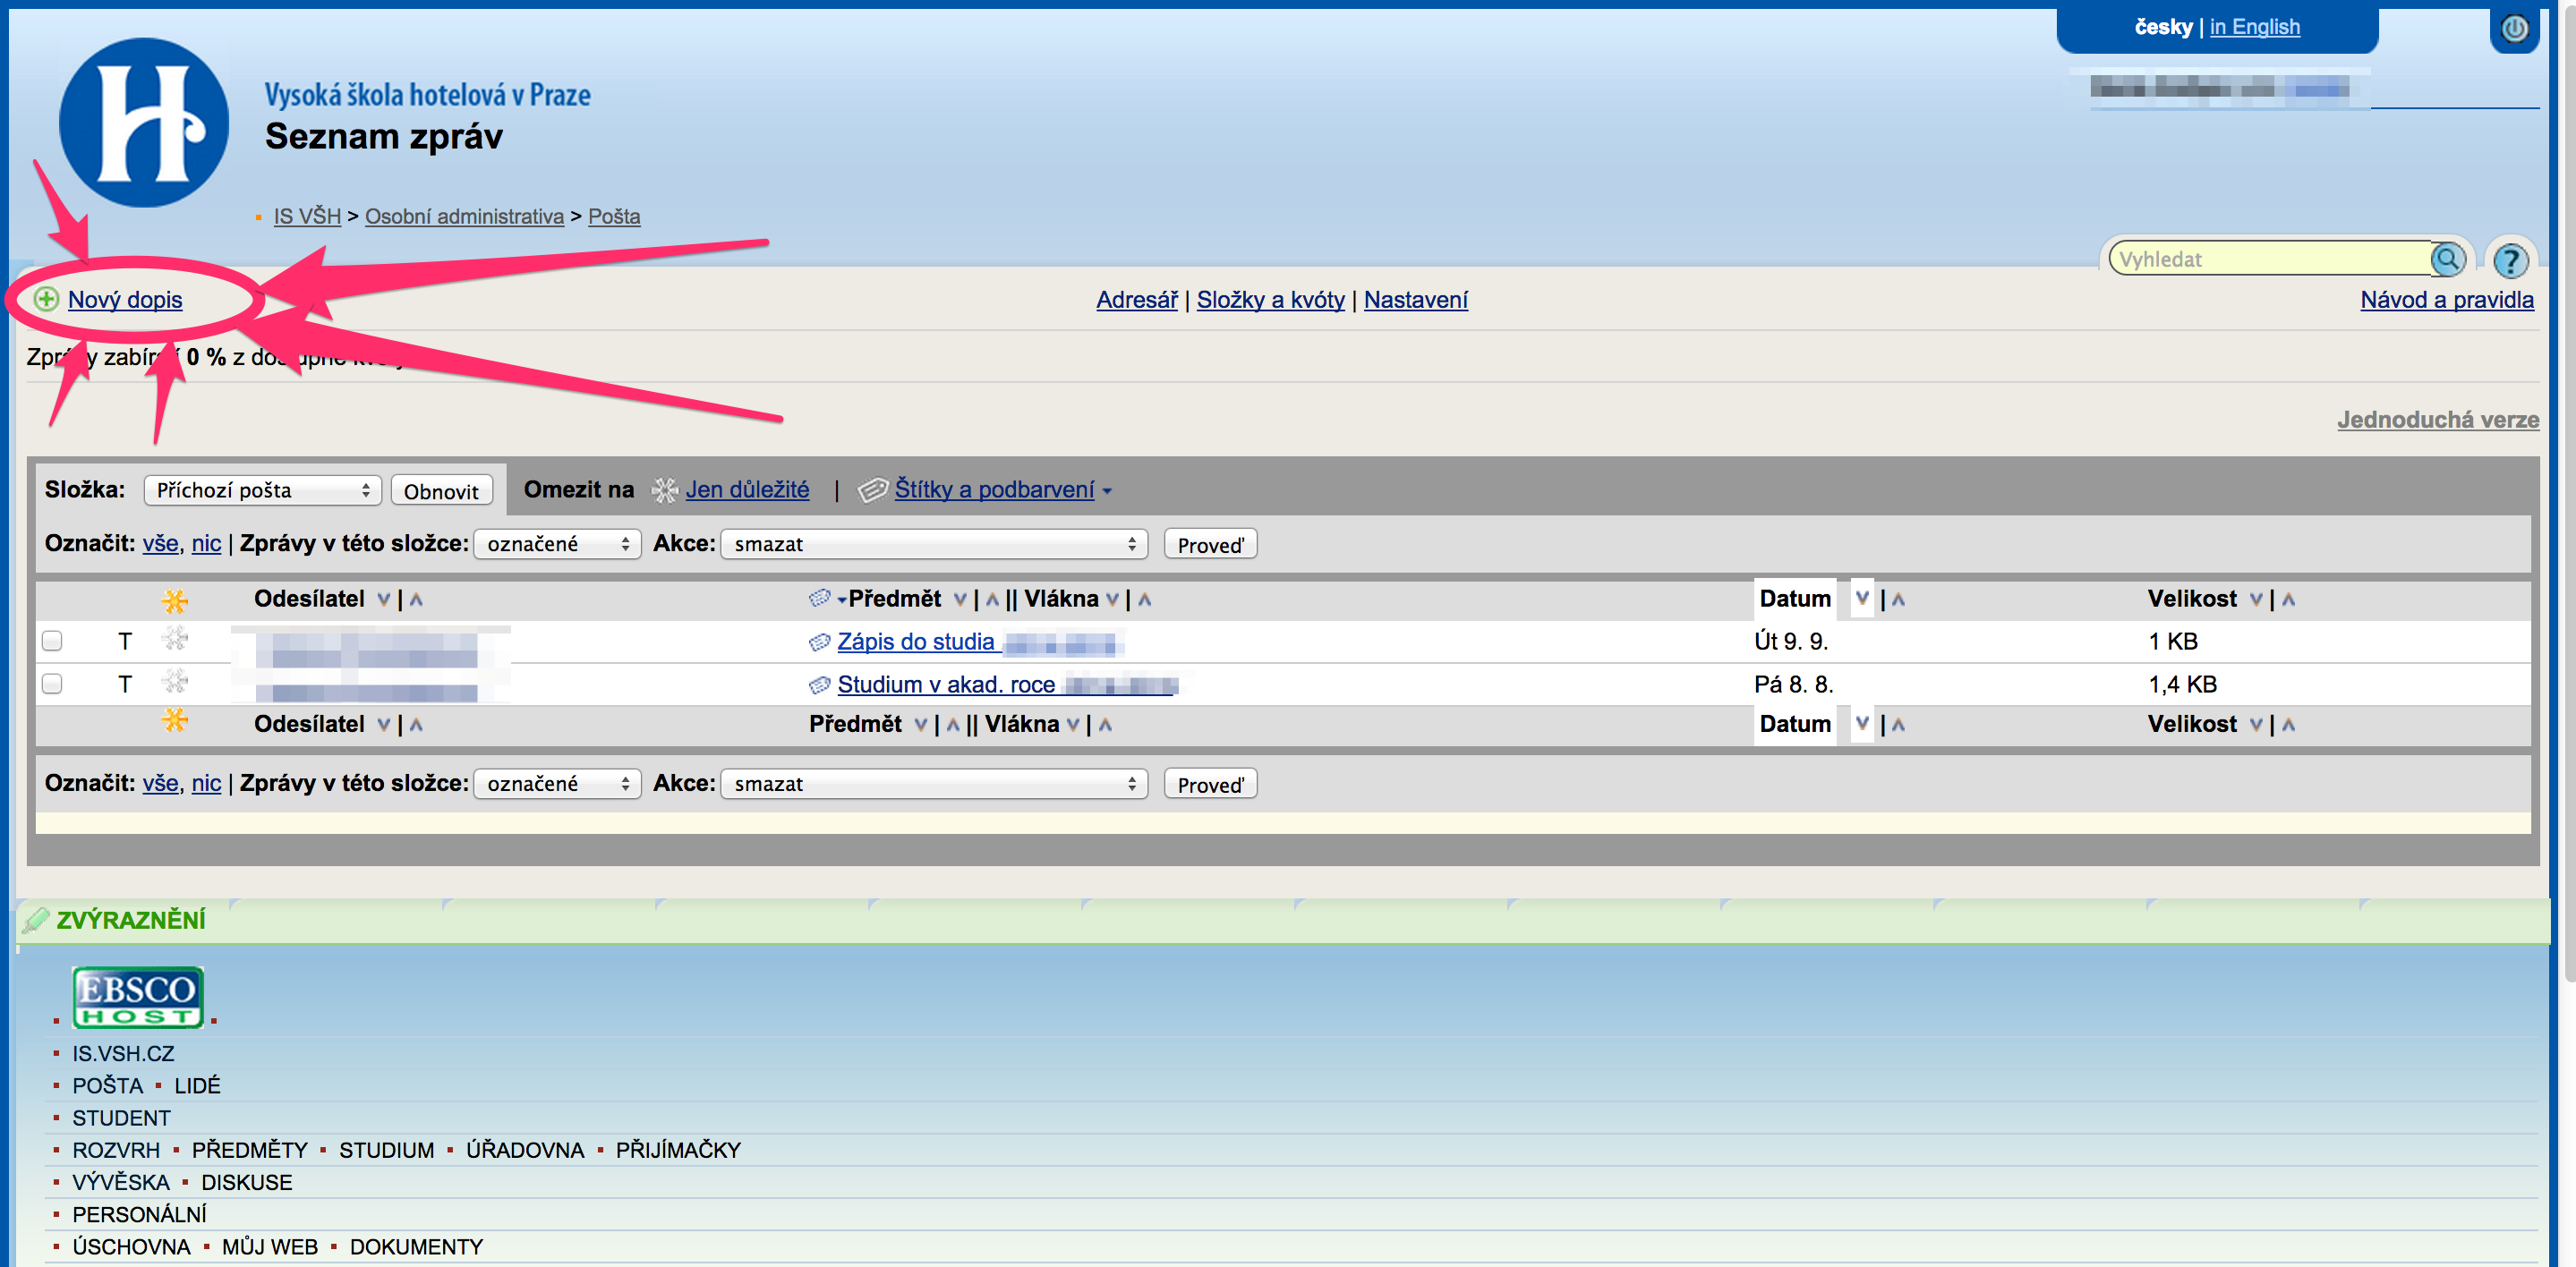
\includegraphics[width=\textwidth]{s09}

\newpage
Budete přesměrováni na novou stránku, 
%\text{kde budete schopni napsat požadovanému člověkovi}. \\

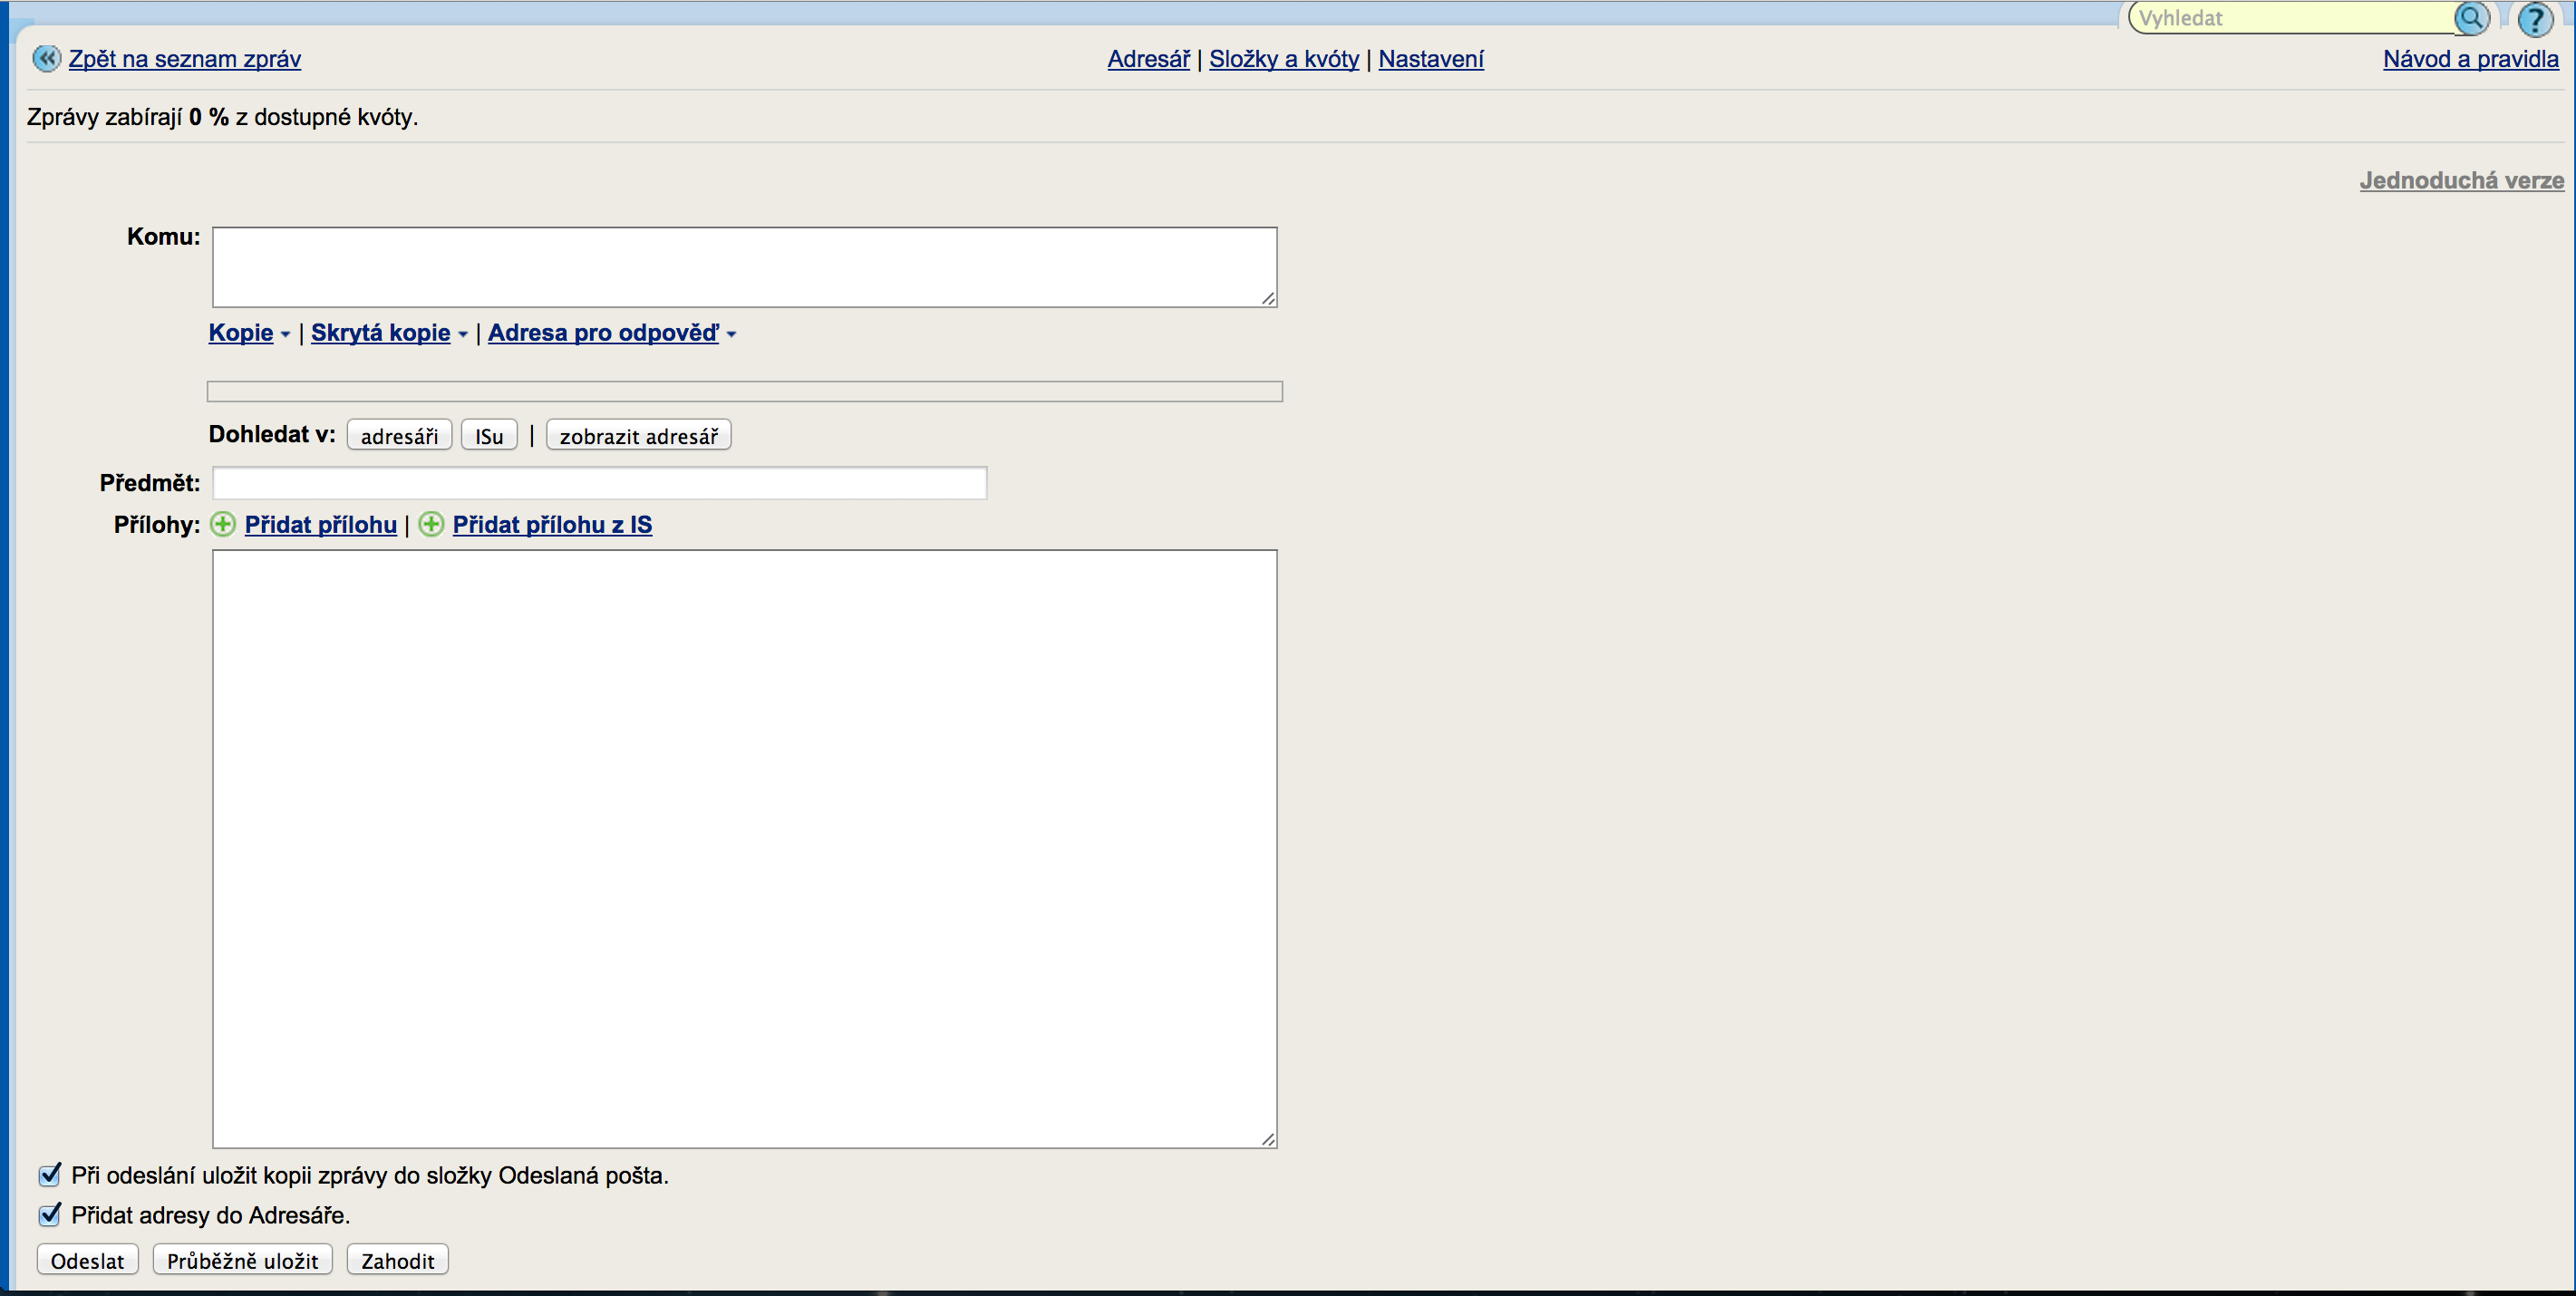
\includegraphics[width=\textwidth]{s10-2} \\

Vzorek dopisu. \\

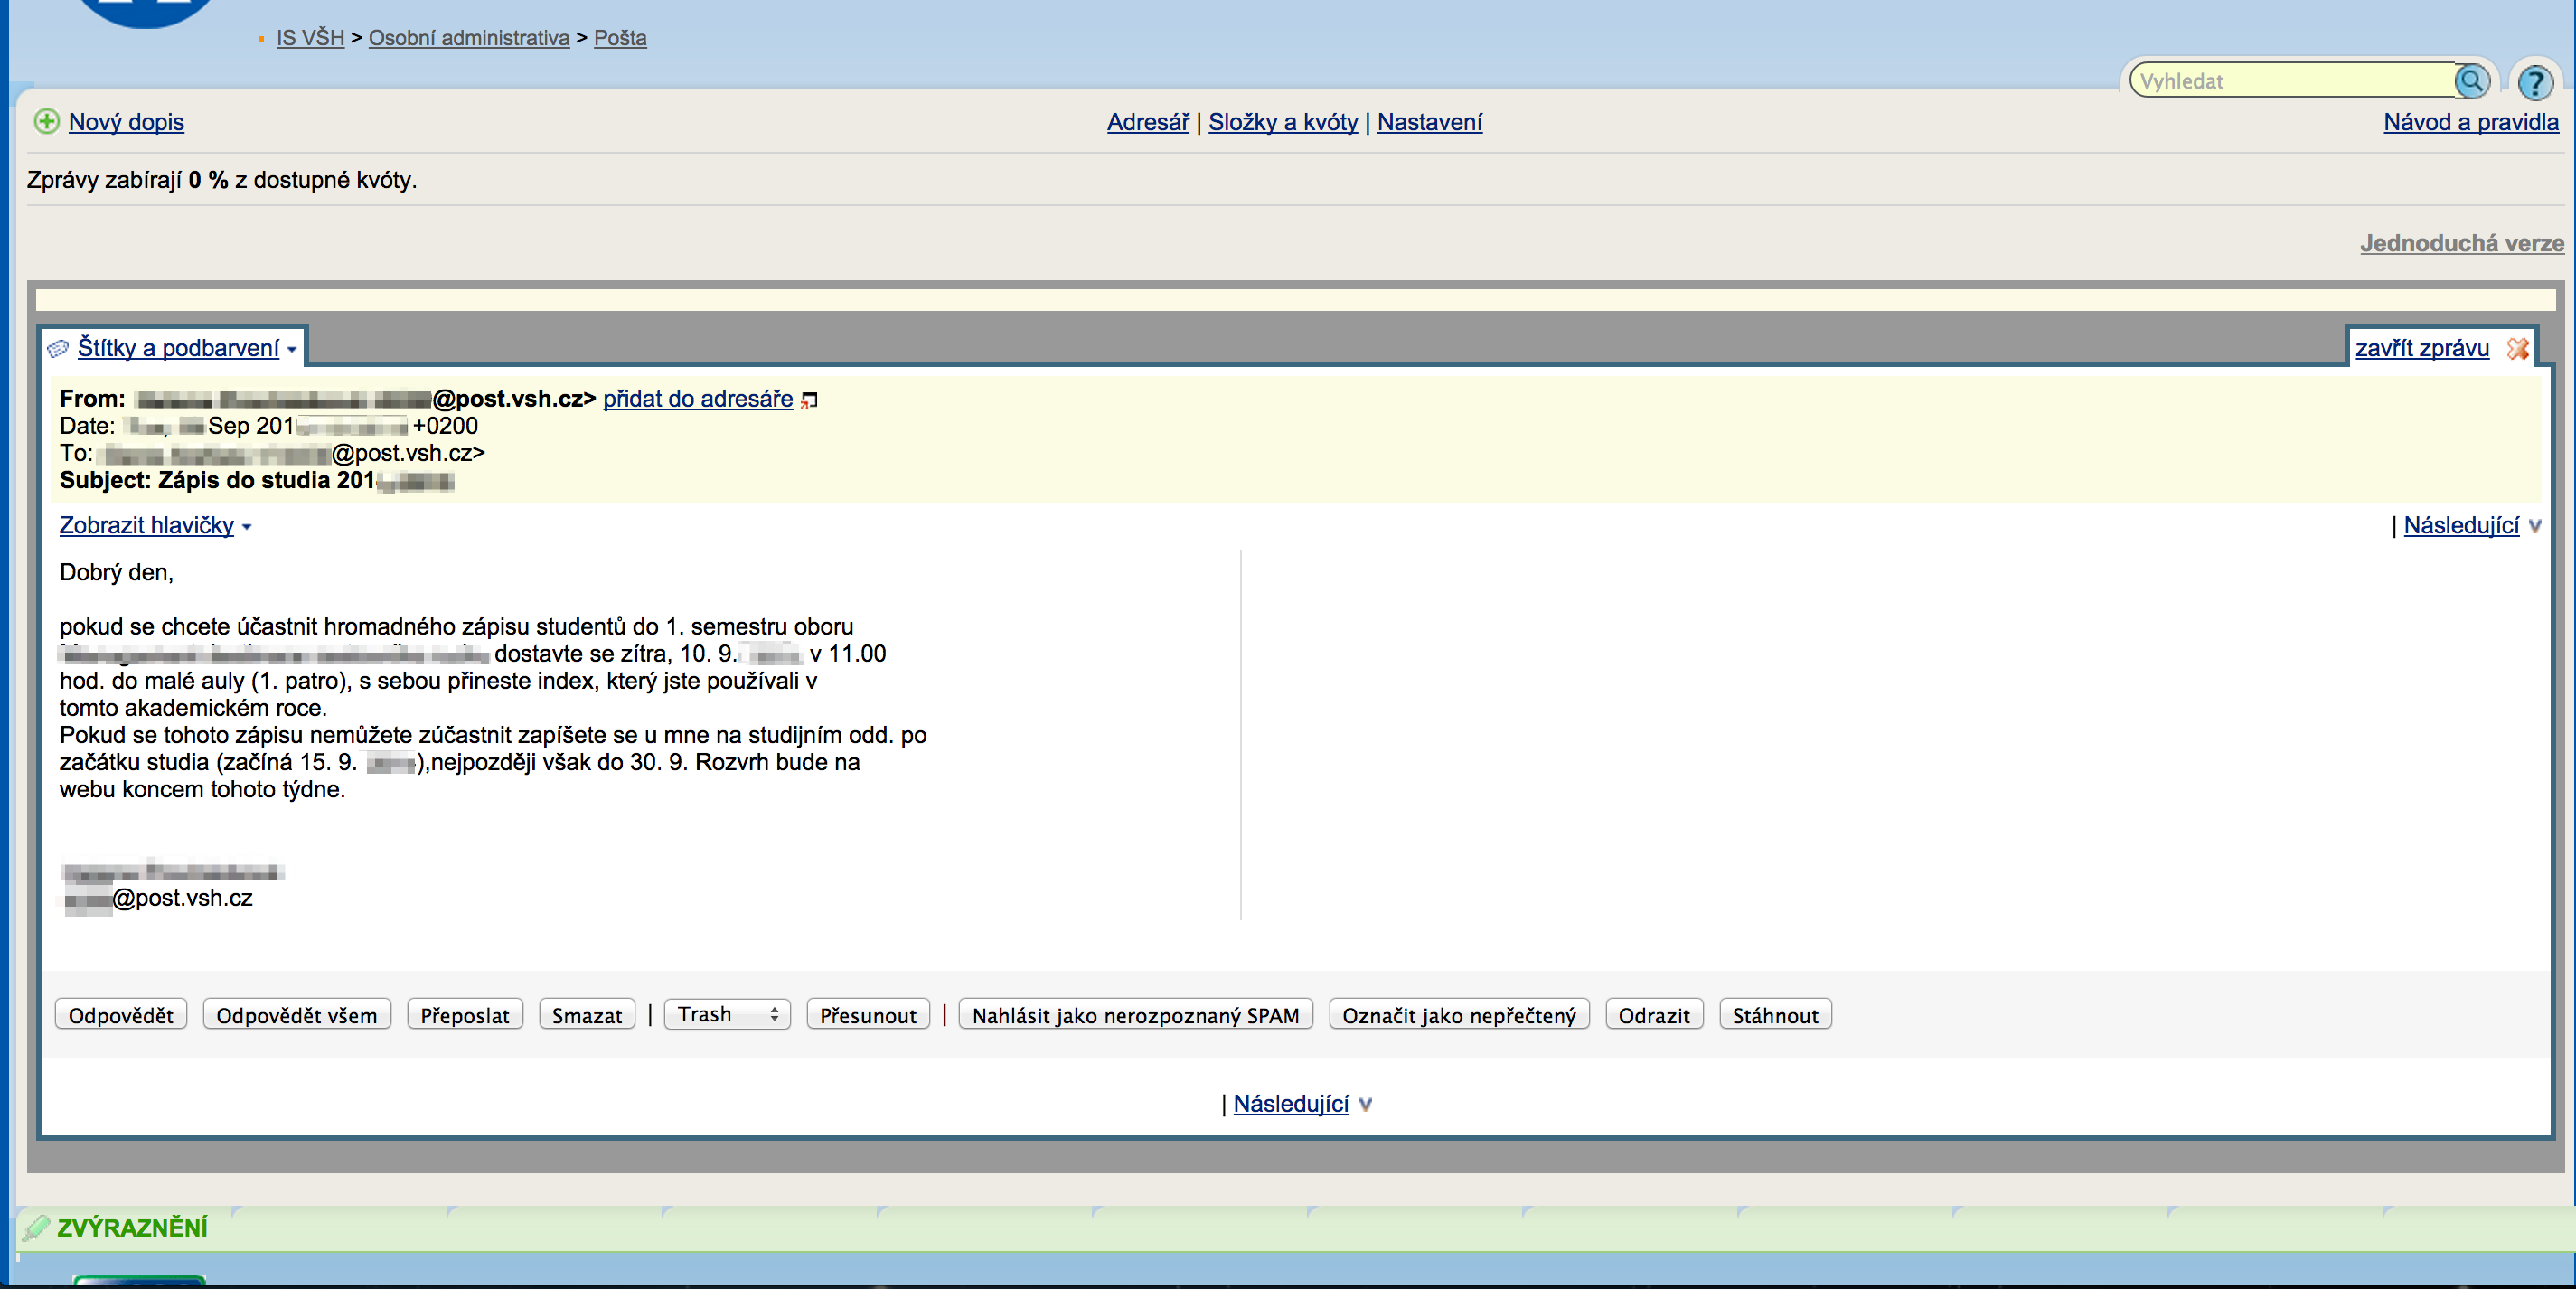
\includegraphics[width=\textwidth]{s10-1}

\newpage

\section{Jak najít správné informace}

Téměř všechny důležité informace jsou uvedeny v sekci
\href{https://is.vsh.cz/auth/vyveska/}{Vývěska} \\

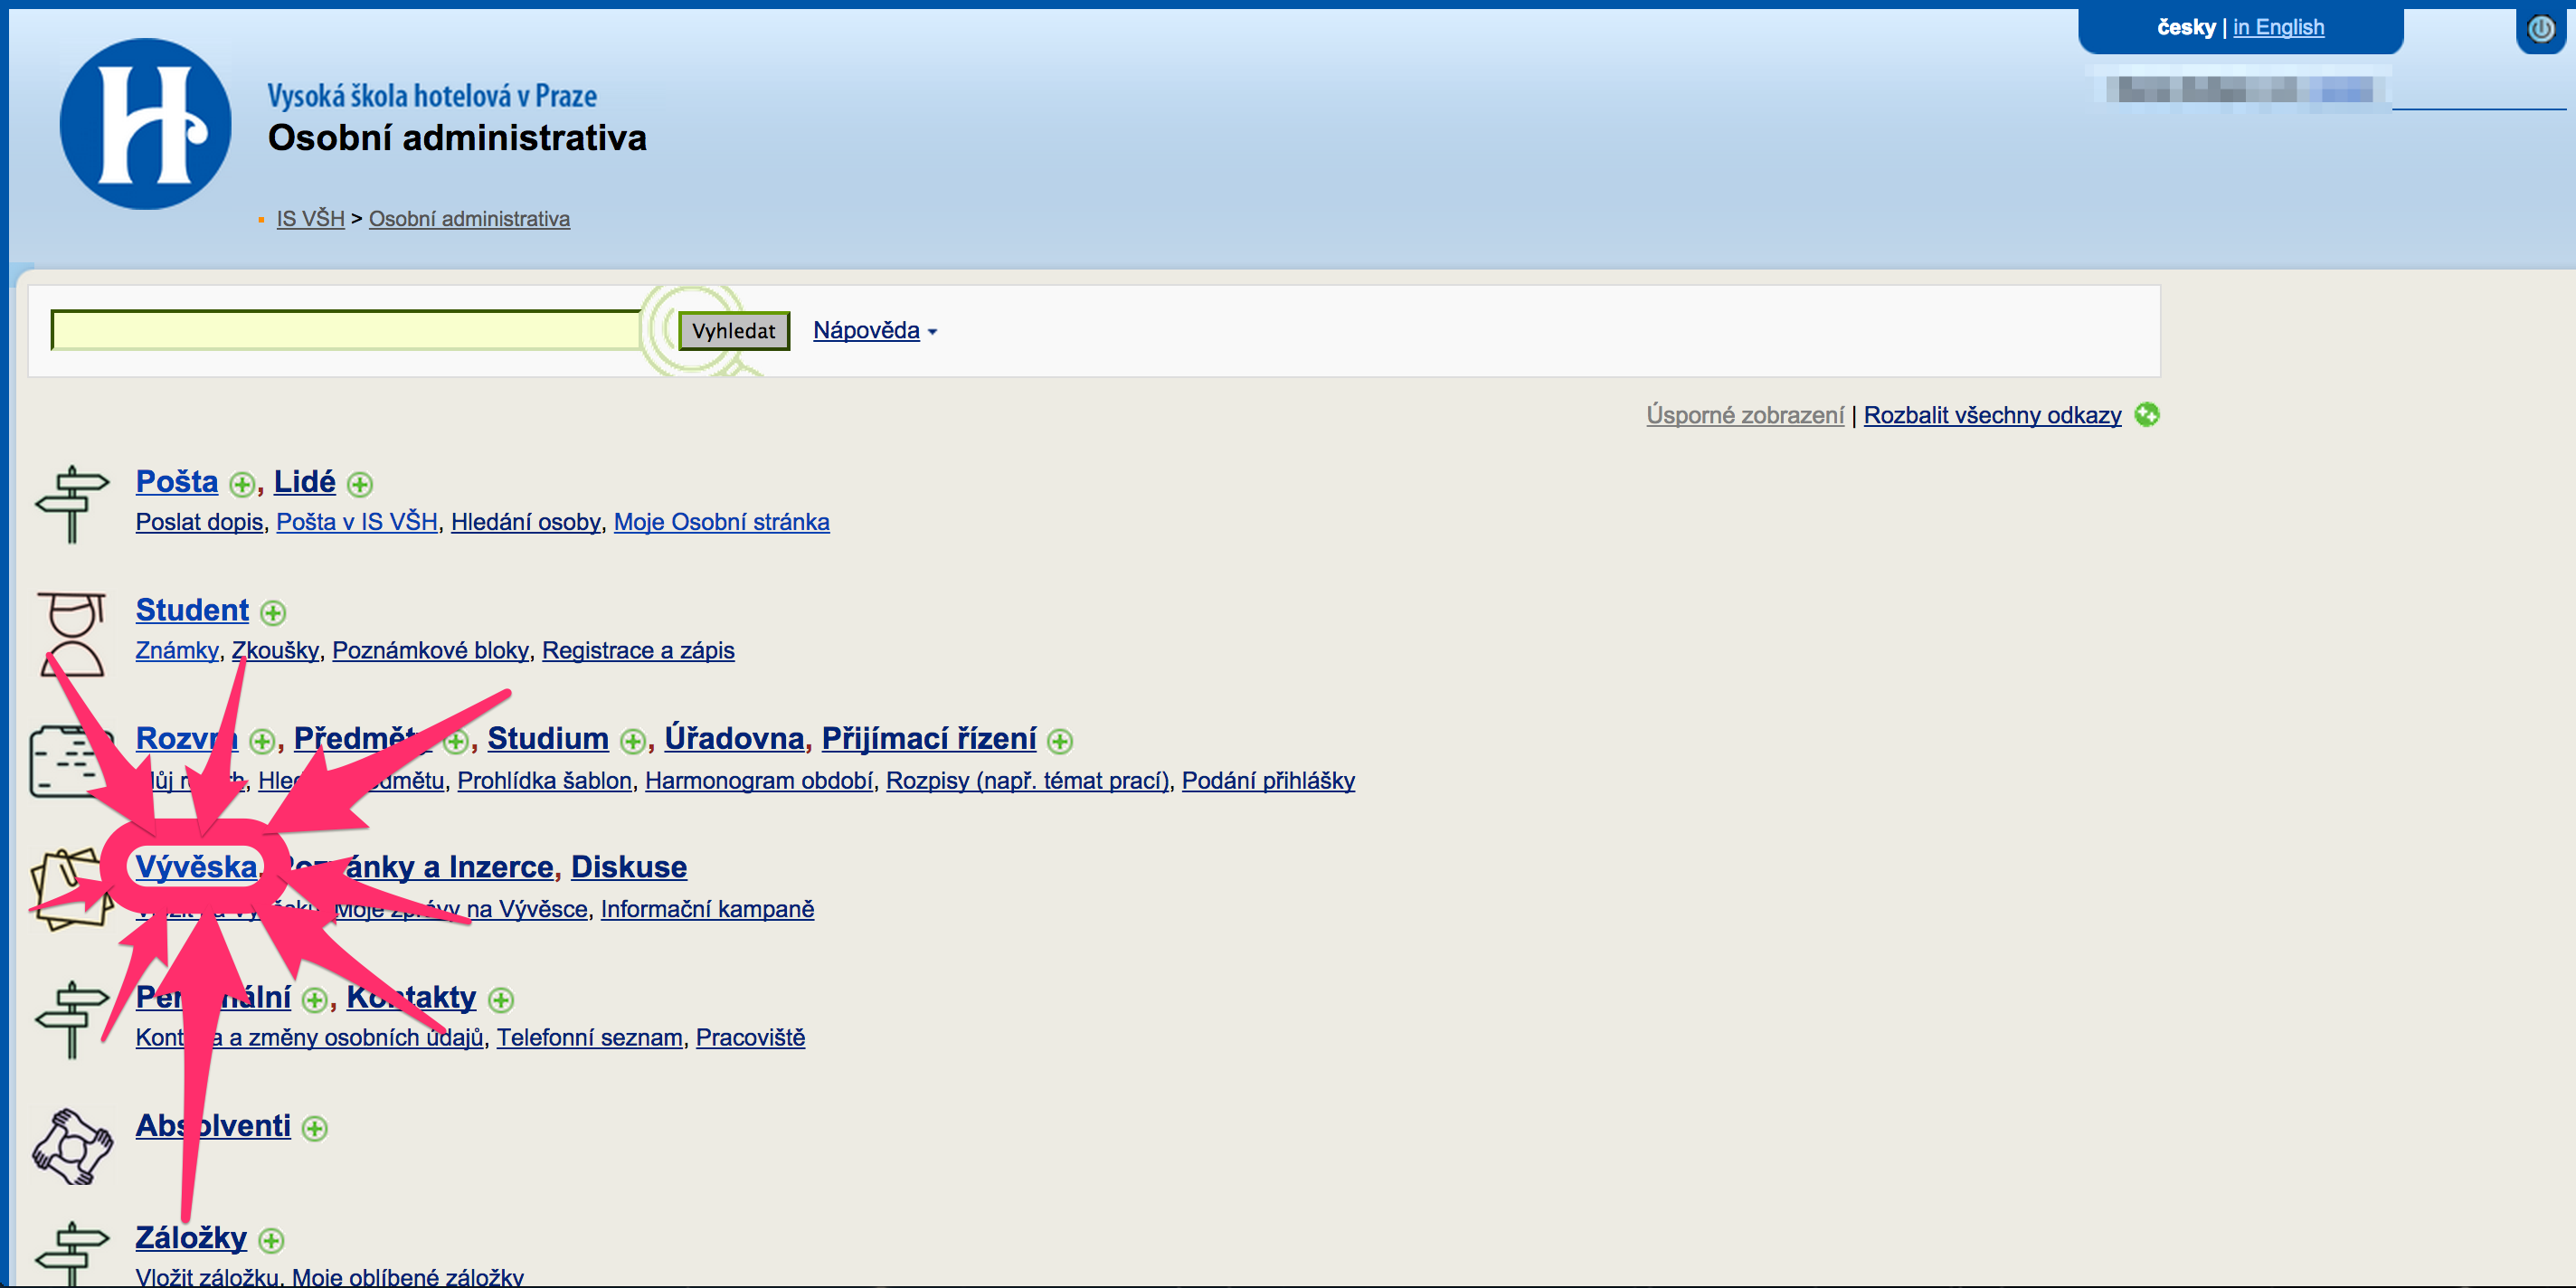
\includegraphics[width=\textwidth]{s11} \\

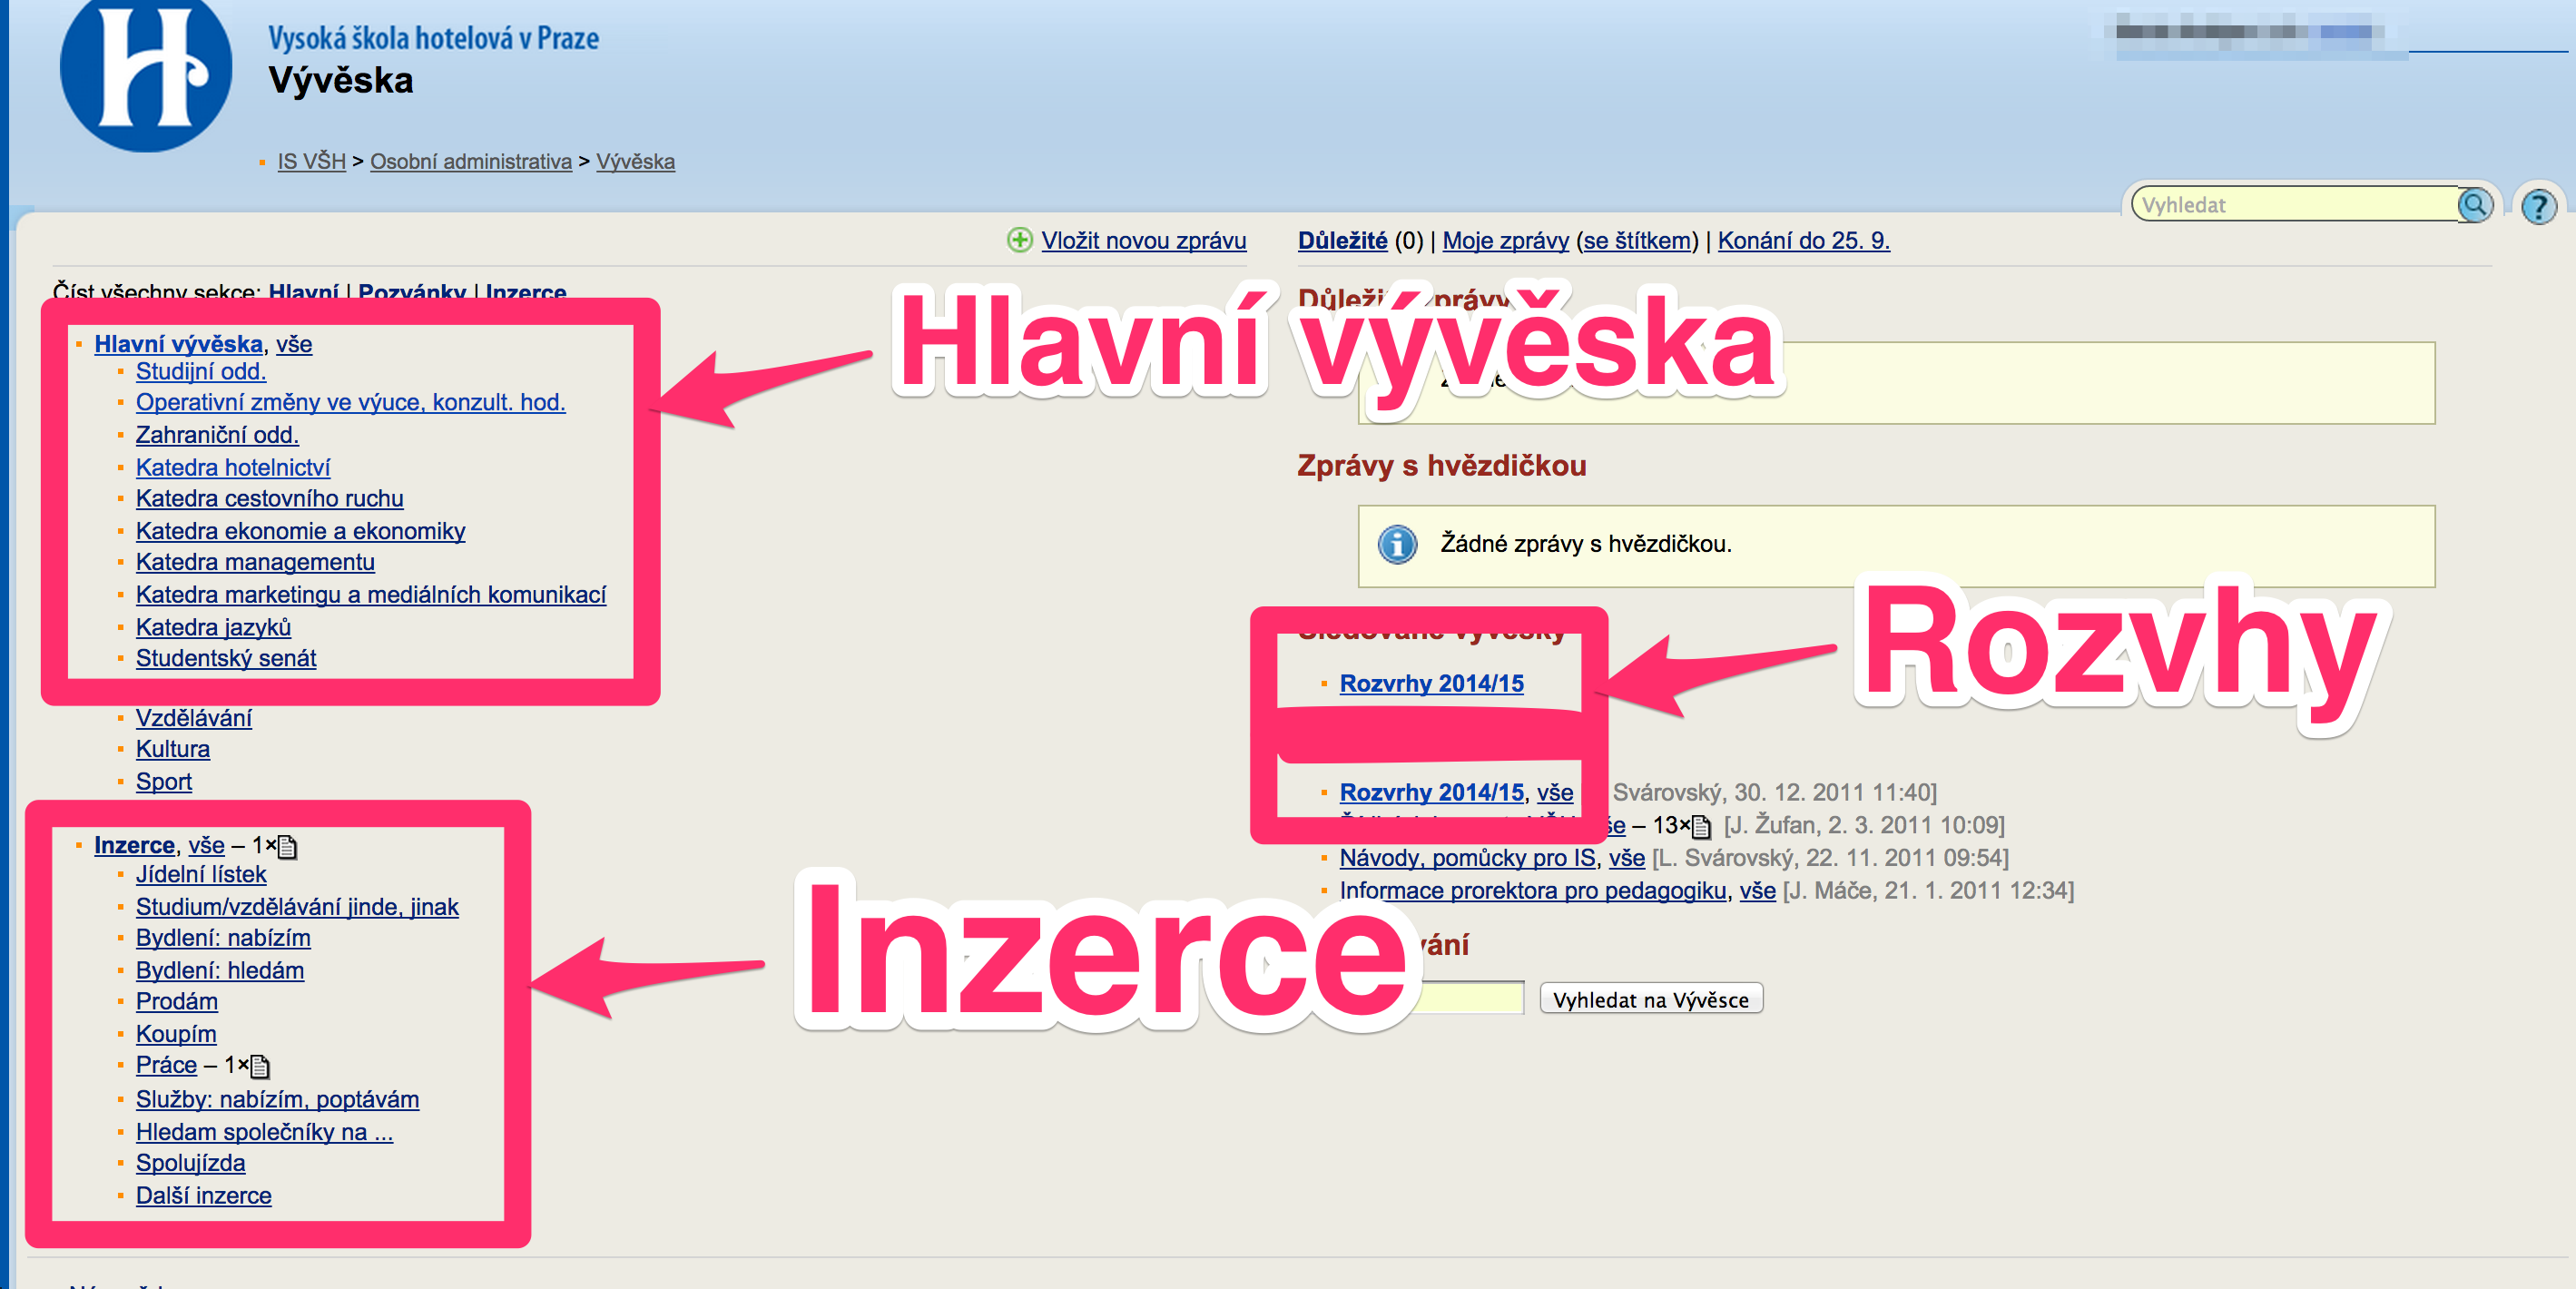
\includegraphics[width=\textwidth]{s12-1} \\

Na této stránce můžete najít dva odkazy na rozvrh, \textbf{Hlavní vývěska} 
v levém horním rohu se zobrazí noviny studentského oddělení, 
fakult, senátu a t.d. Nikdy nezapomínejte na tenhle oddil mrknout ještě jednou. 
Všechny kritické zprávy najdete zde.

Pod \textbf{Hlavní vývěskou} vývěskou je sekce \textbf{Inzerce}, в 
kde můžete najít informace o práci, 
nákupu / prodeji různých vzdělávacích materiálů, a dokonce i pronájmu bytů.

\newpage

\subsection{Rozvrh}
Chcete-li zjistit svůj rozvrh, musíte jít do sekce \href{https://is.vsh.cz/auth/vyveska/}{Vývěska}
a klikněte na jeden ze dvou odkazů \textbf{Rozvrhy} \\

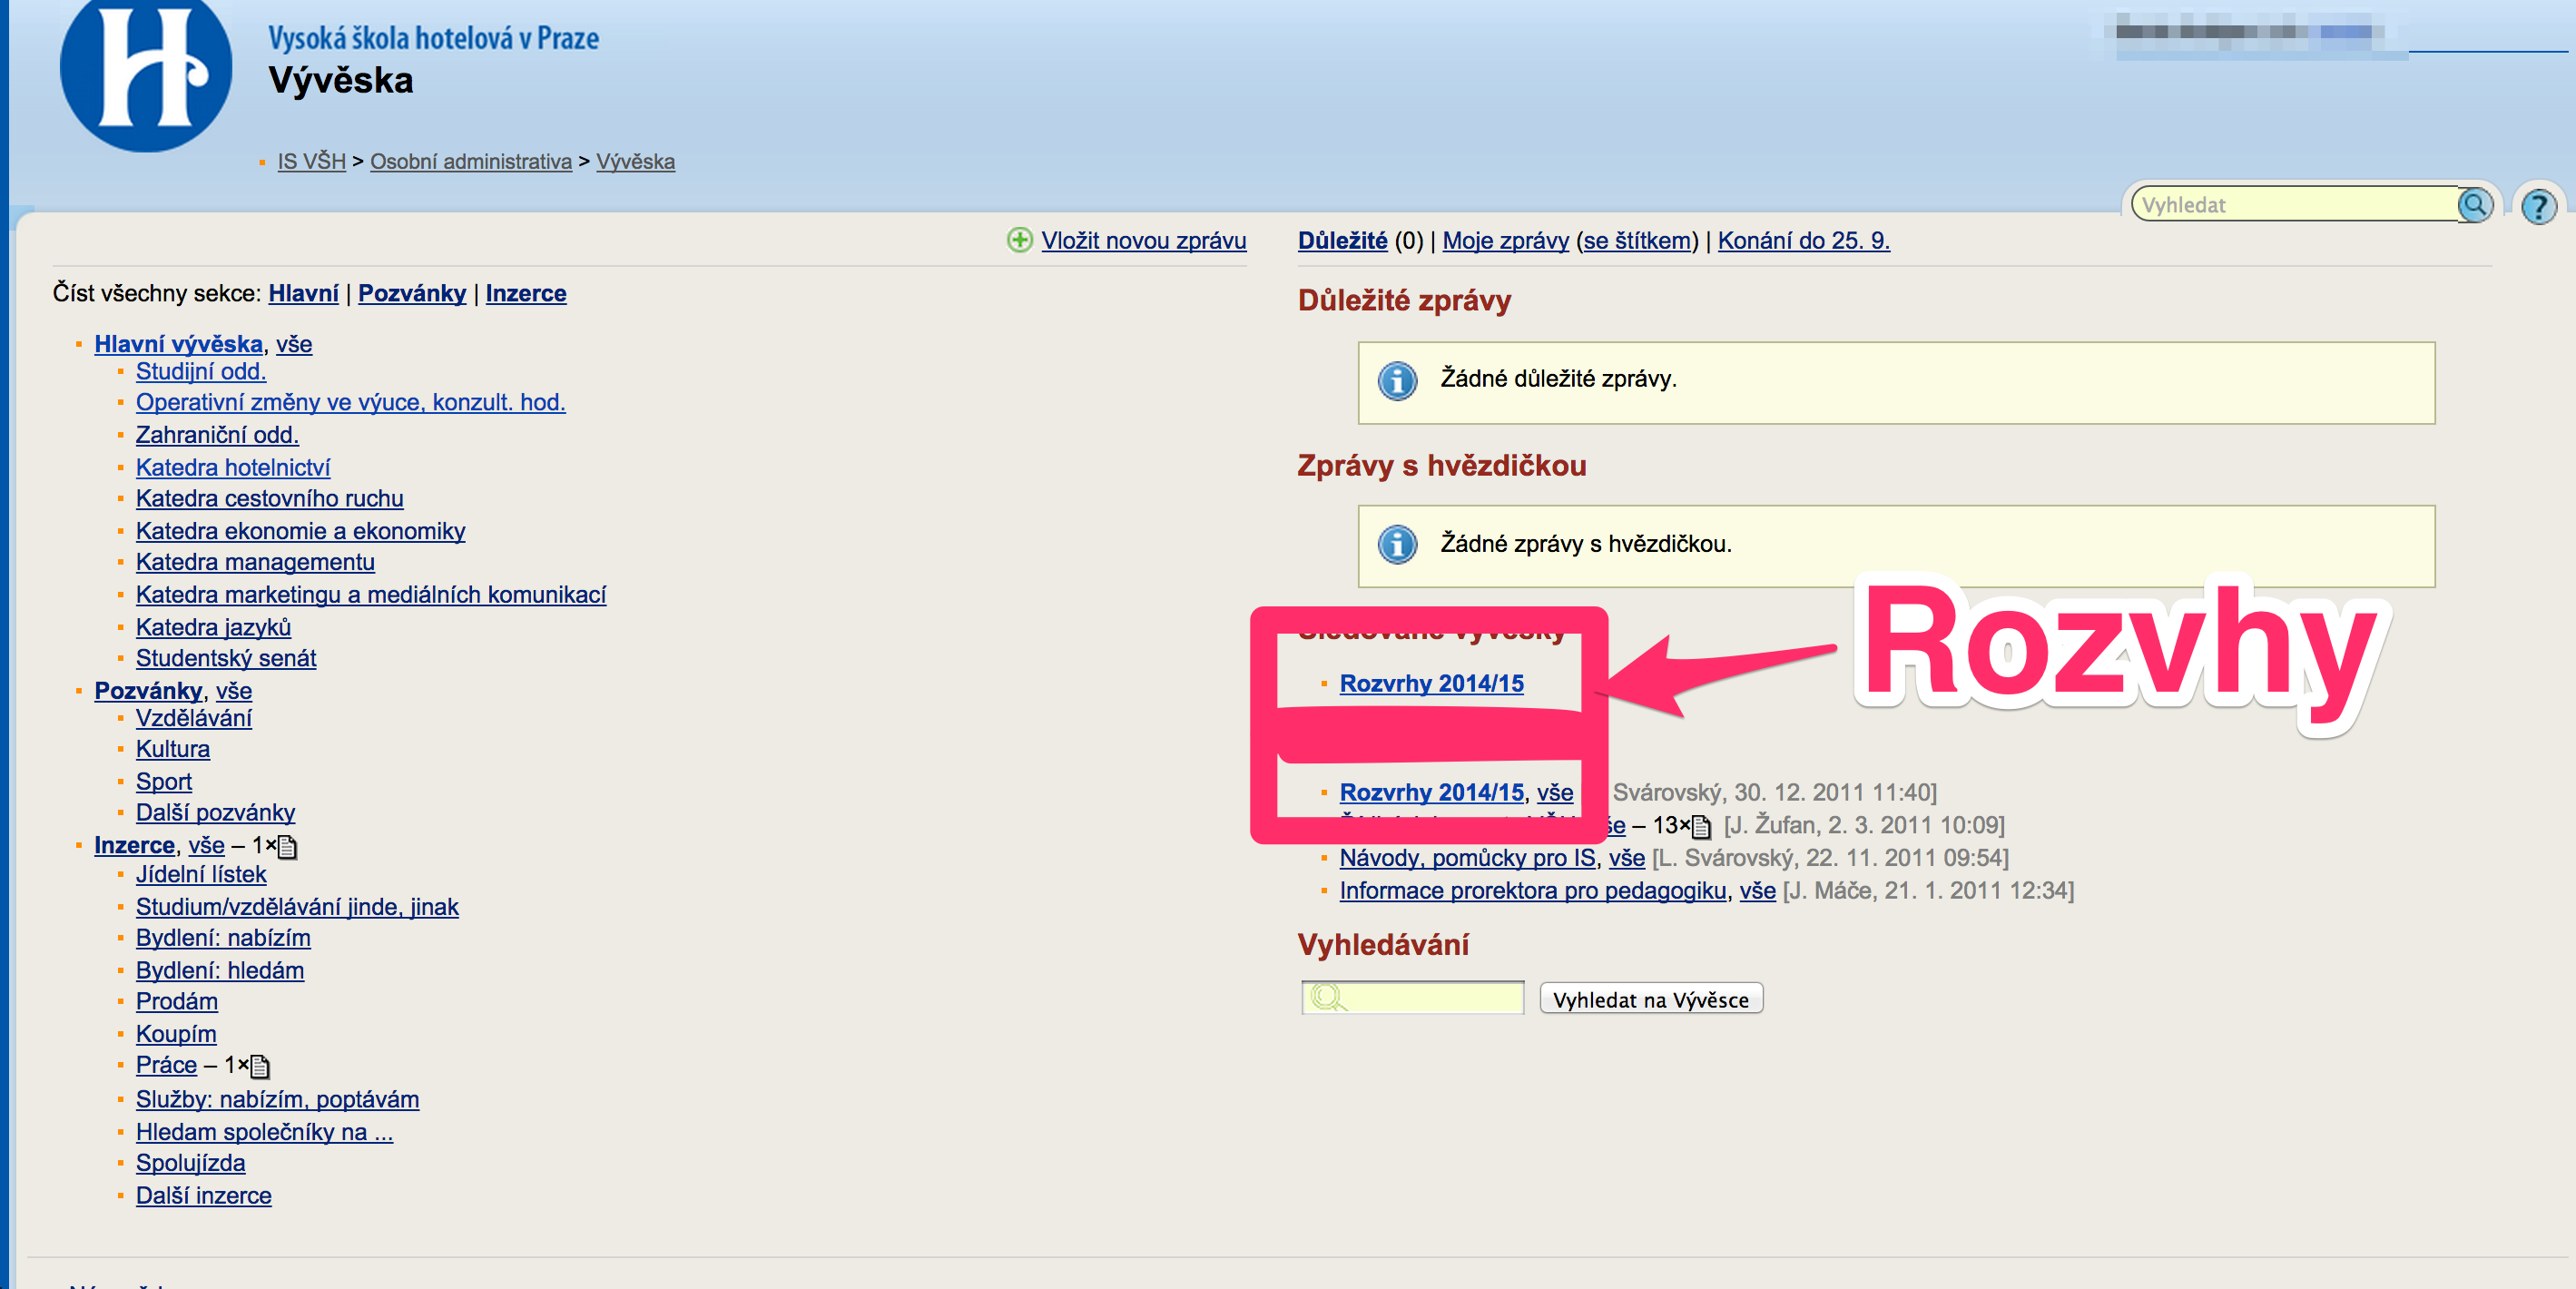
\includegraphics[width=\textwidth]{s13-1} \\

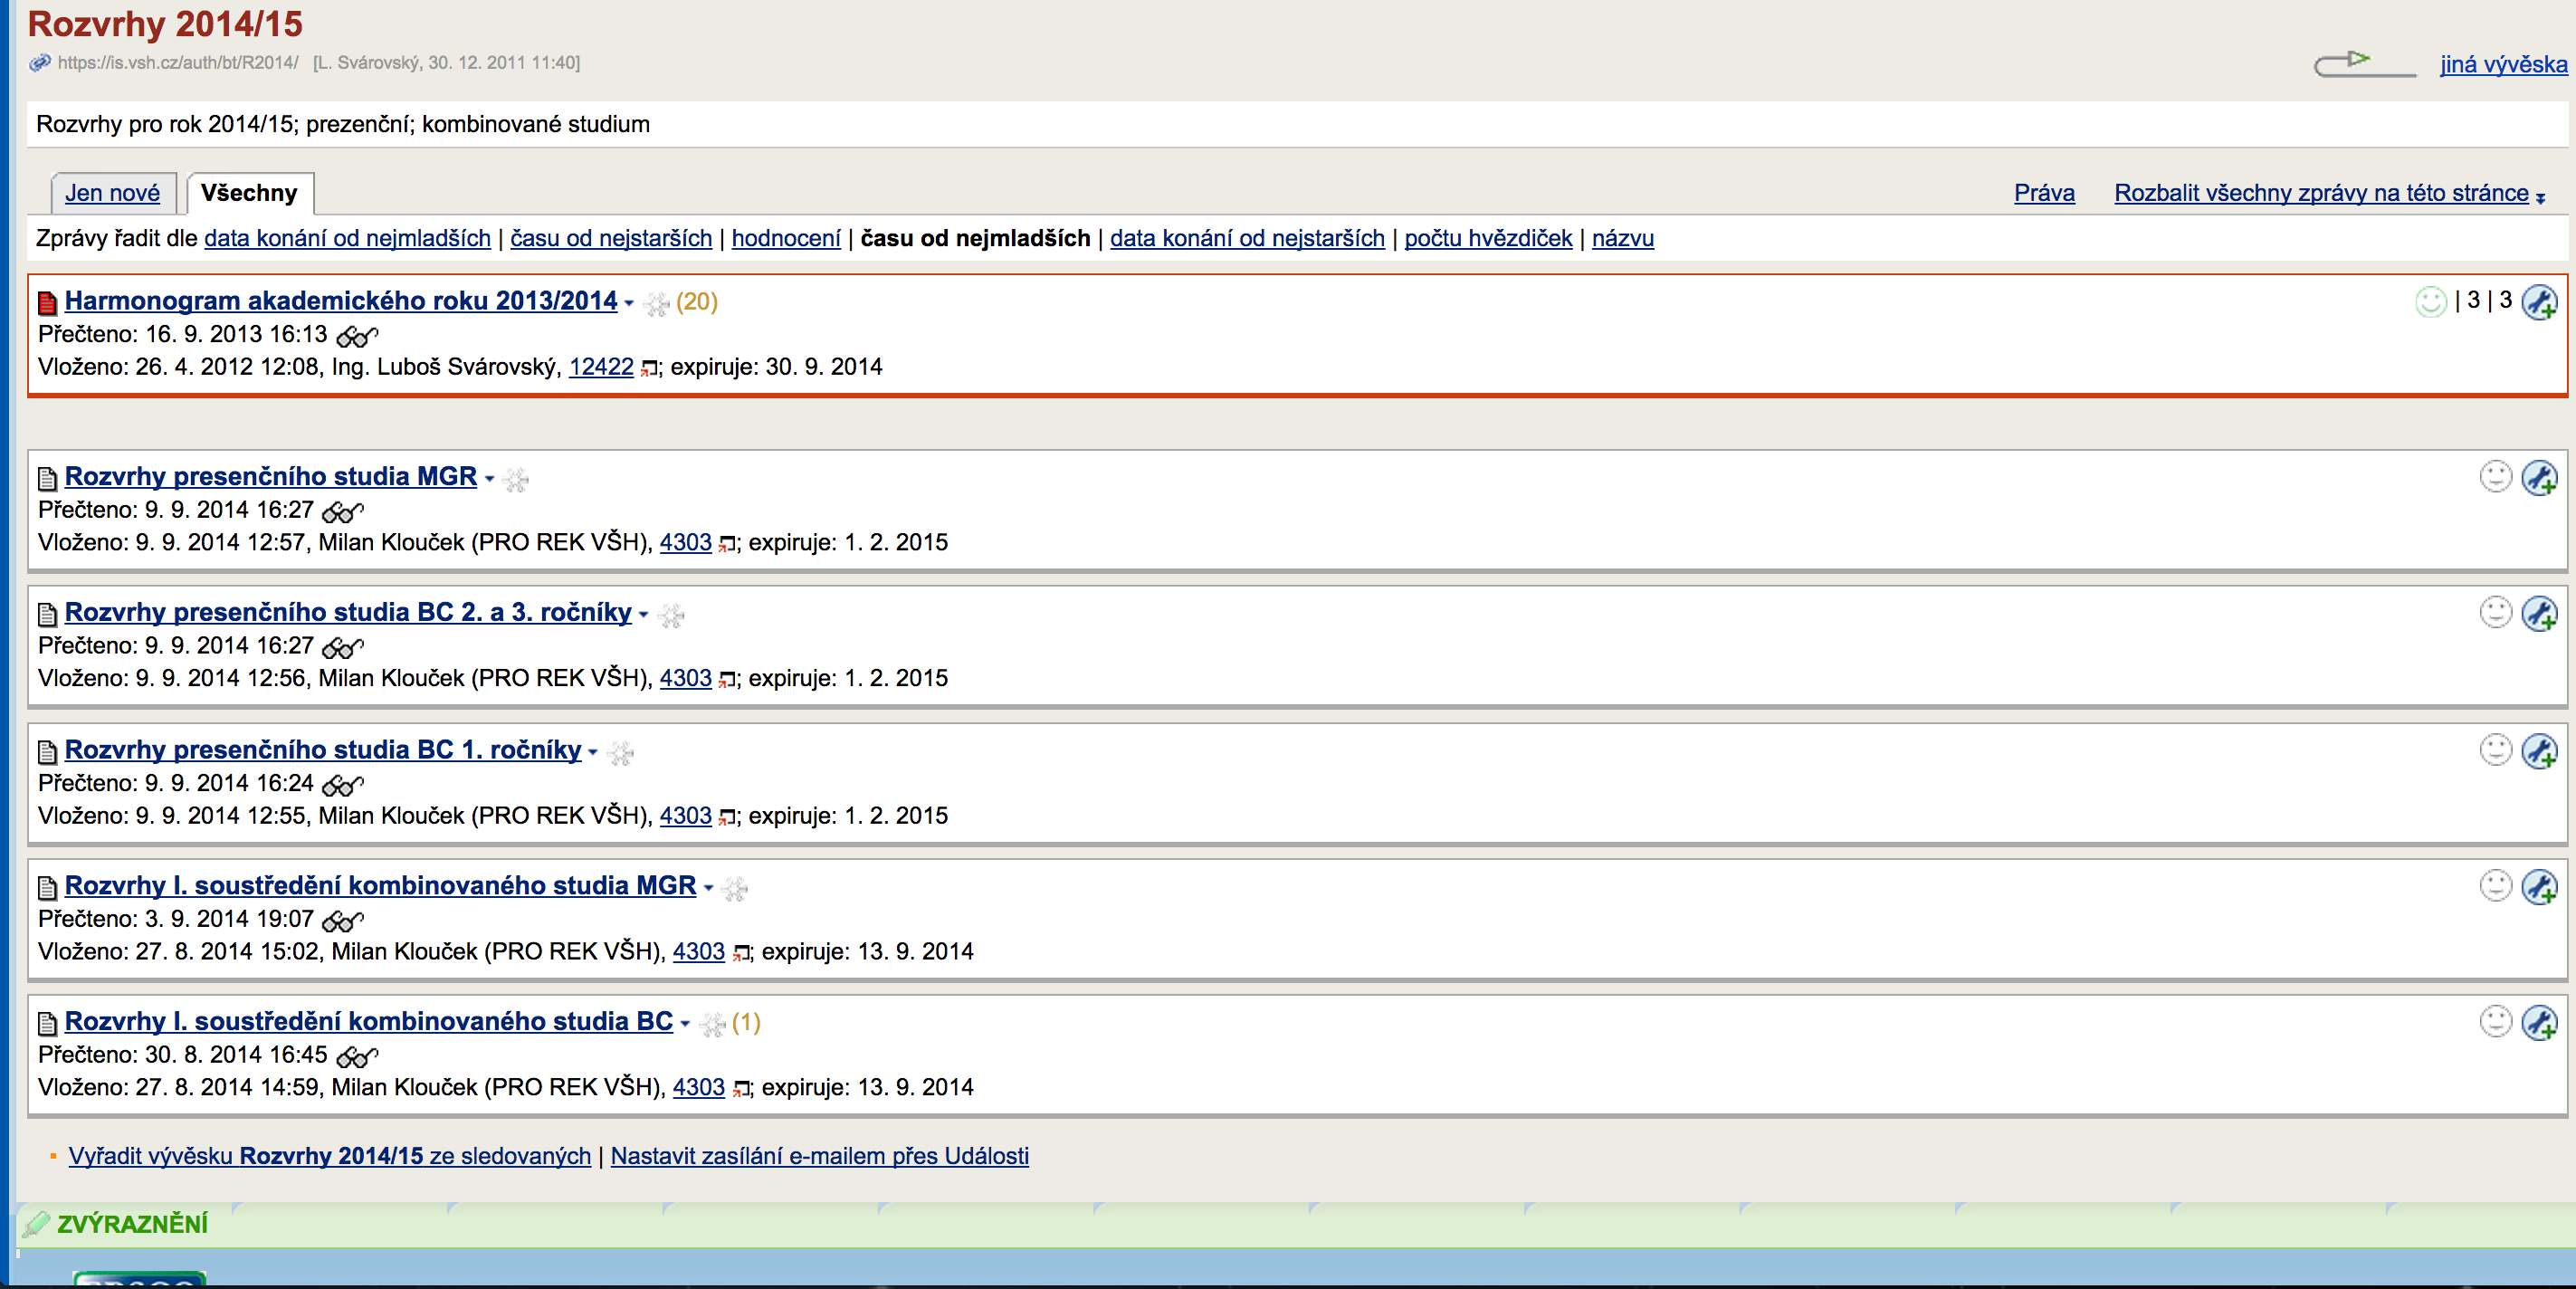
\includegraphics[width=\textwidth]{s14} \\

\newpage

Zde jsou rozvrhy všech fakult, kateder a let, takže byste měli přesně vědět, 
jaký rozvrh potřebujete. 
Snadná navigace pro takový případ není k dispozici. \\

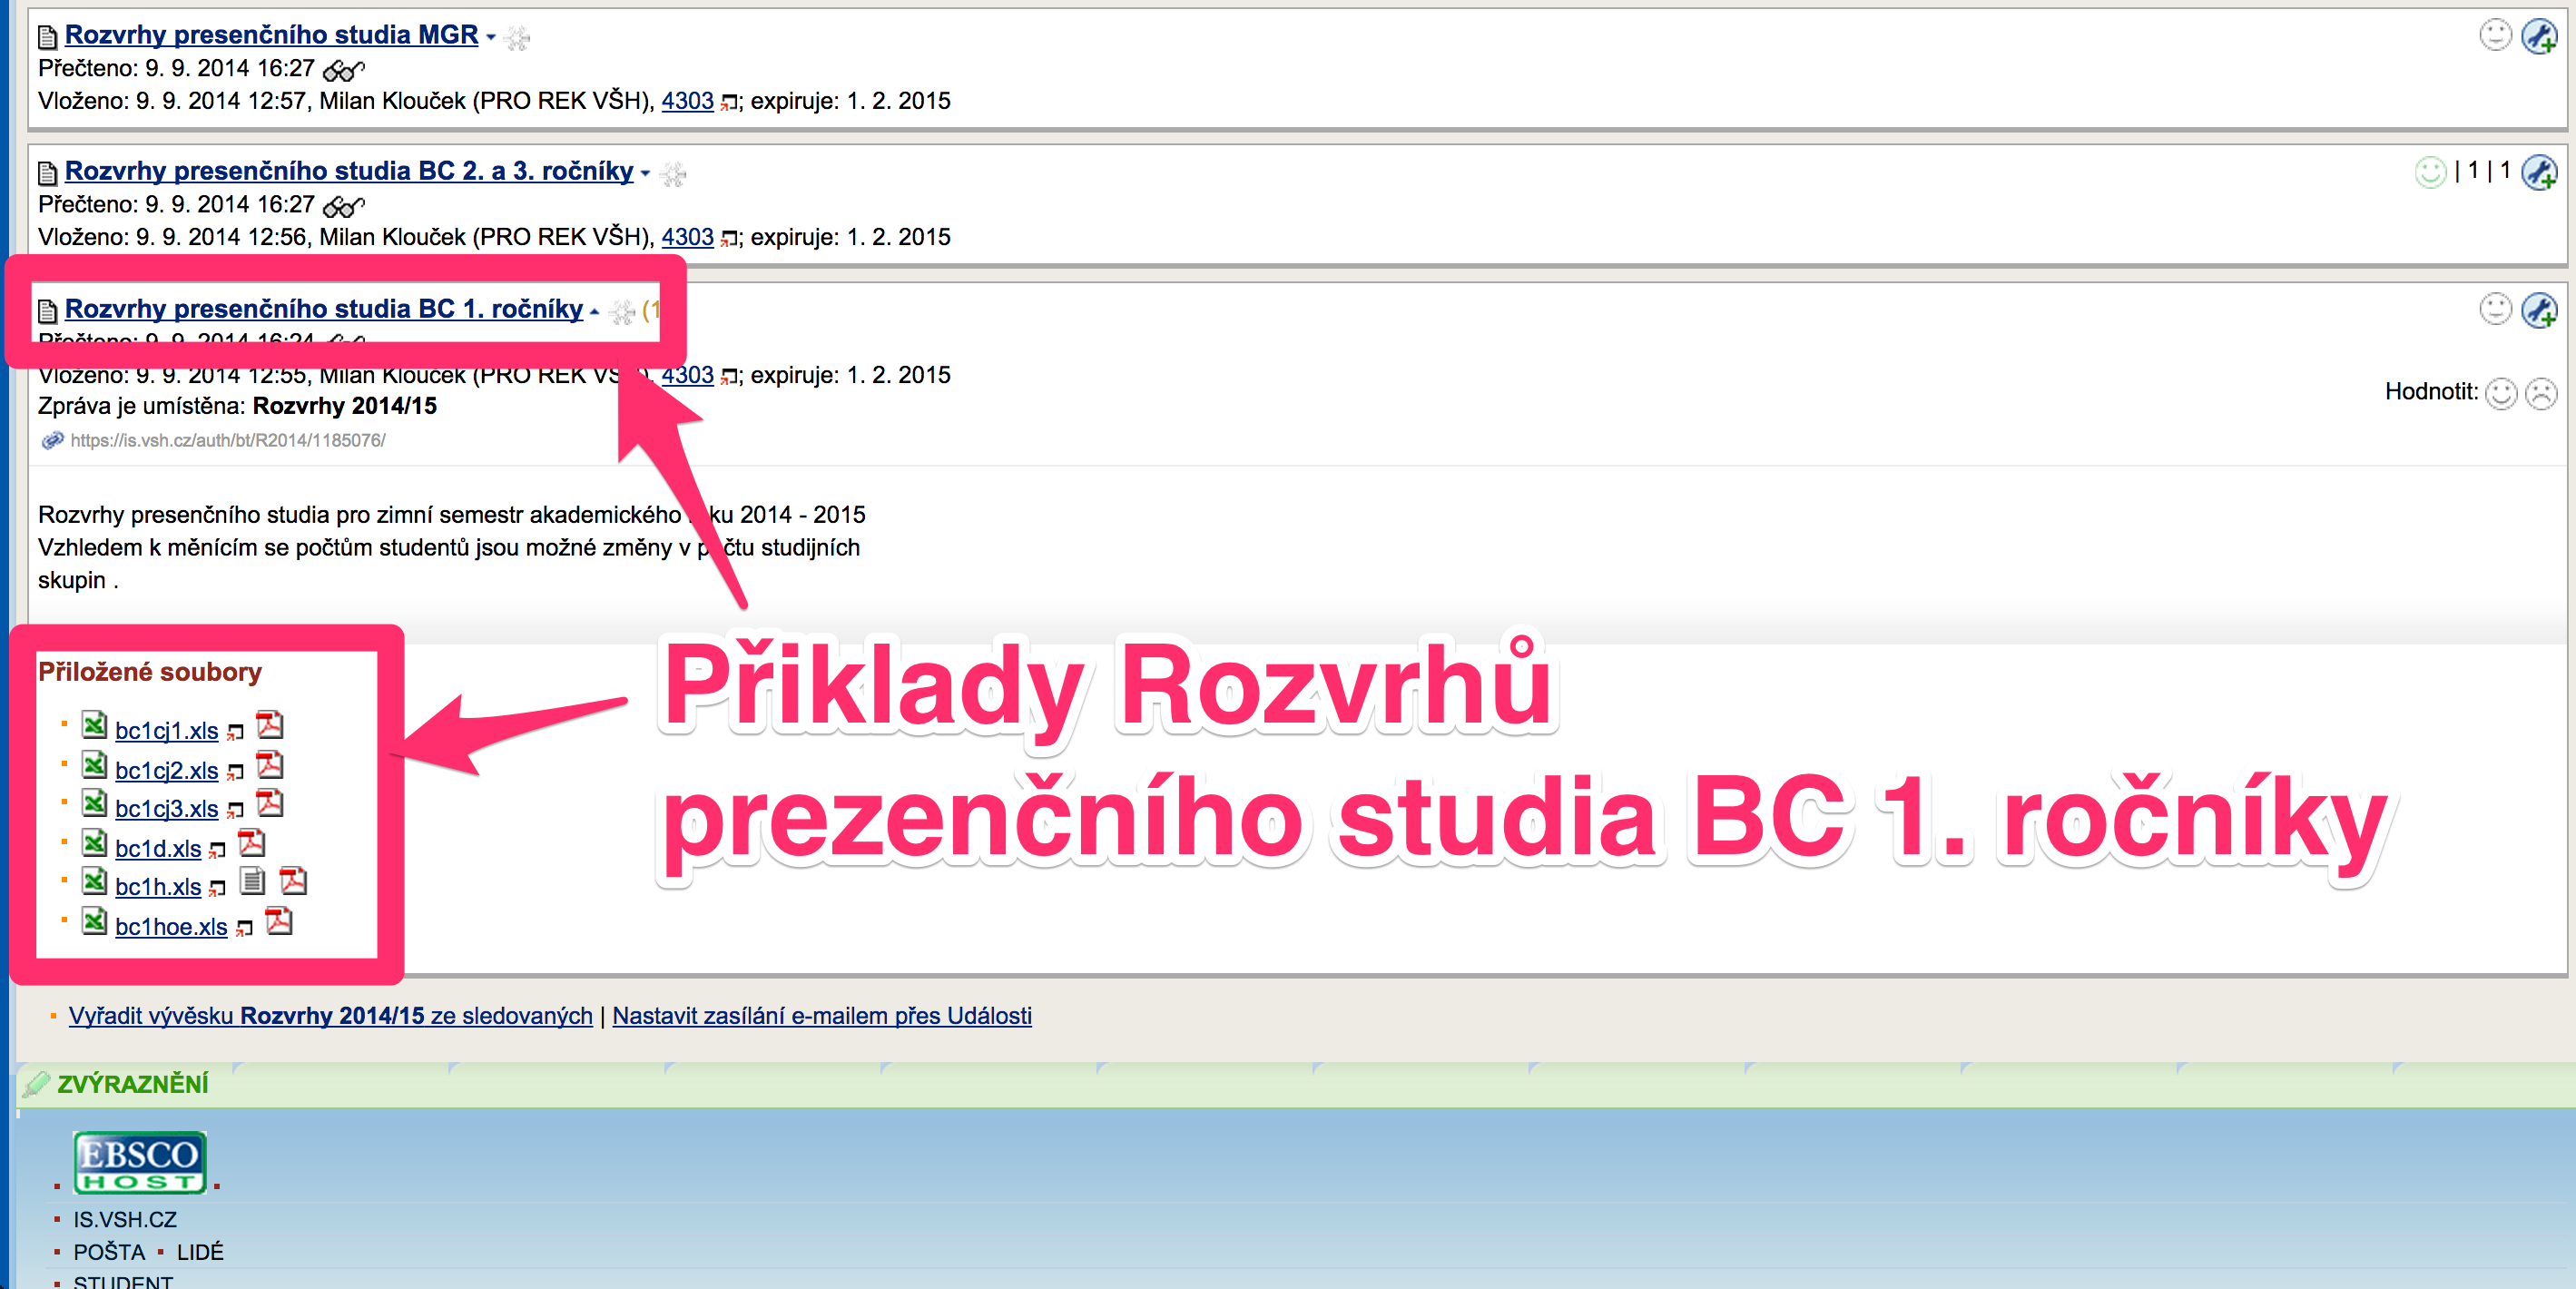
\includegraphics[width=\textwidth]{s15-1}

	\subsection{Příklad Rozvrhu}

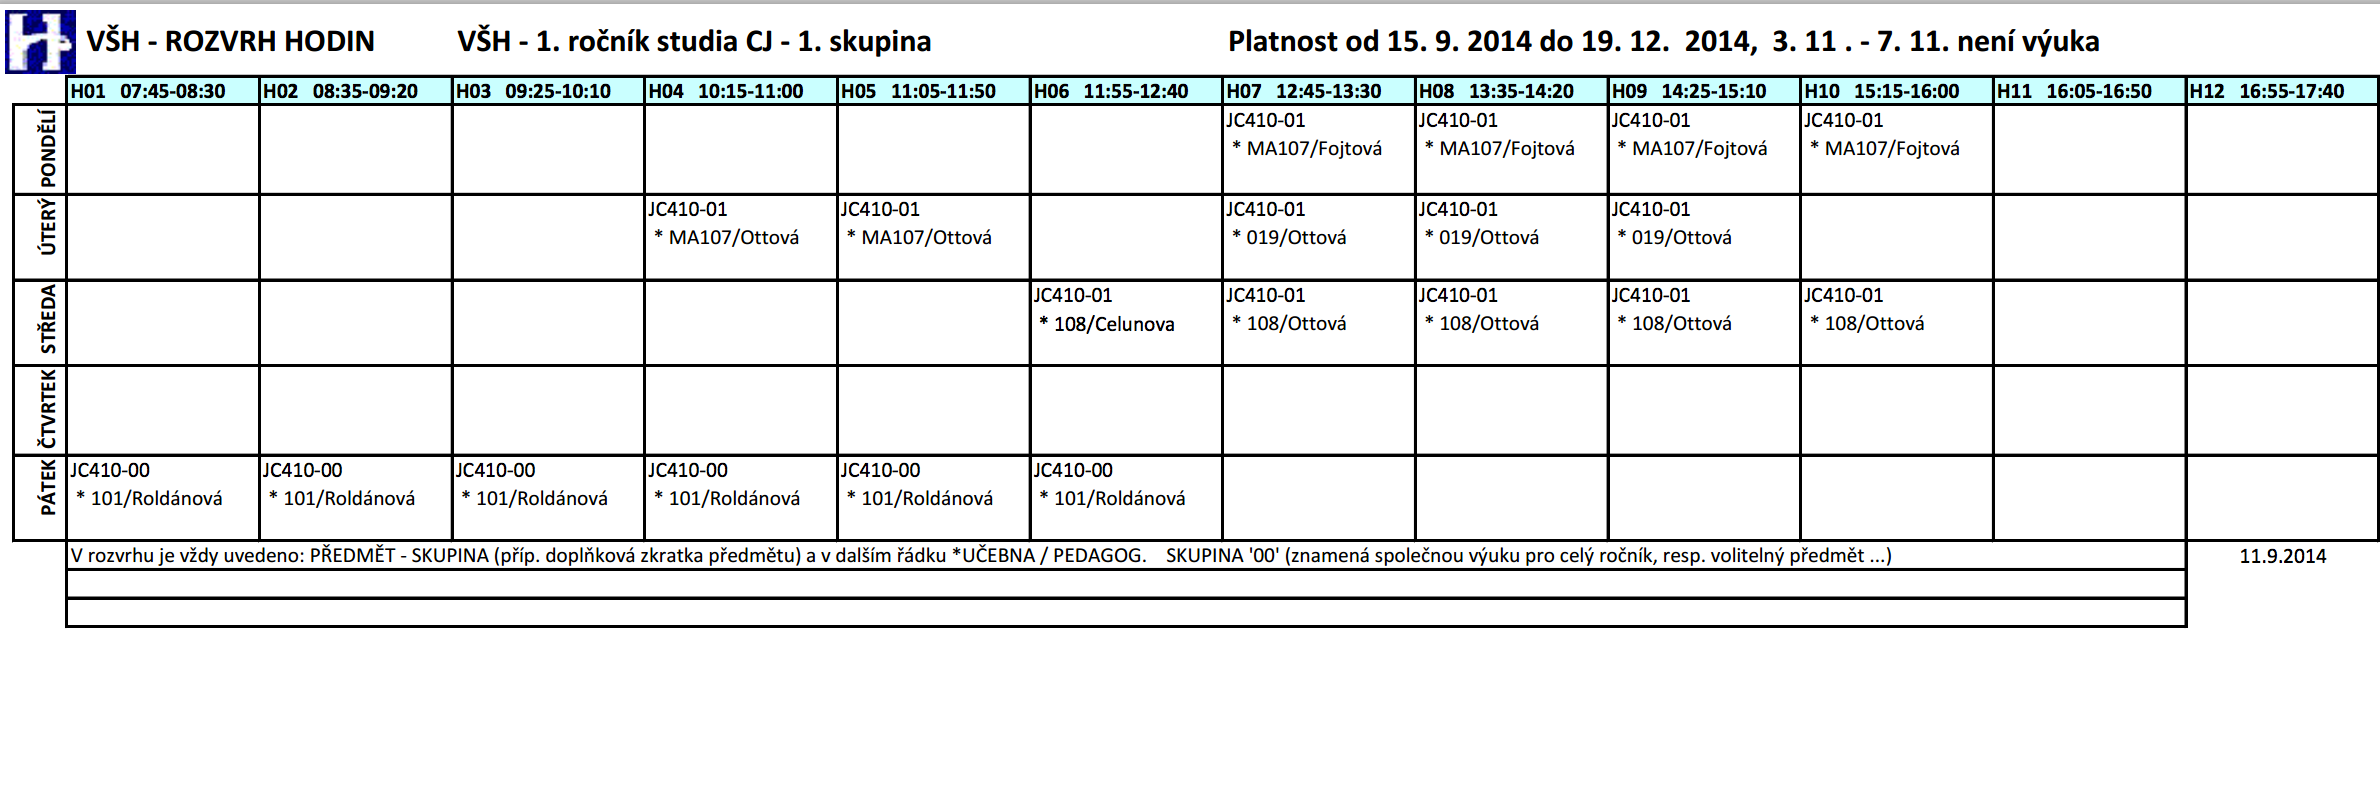
\includegraphics[width=\textwidth]{s16} \\

\newpage

\section{Známky a školné}

Nyní uvažujme oddíl \href{https://is.vsh.cz/auth/student/}{Student}. \\

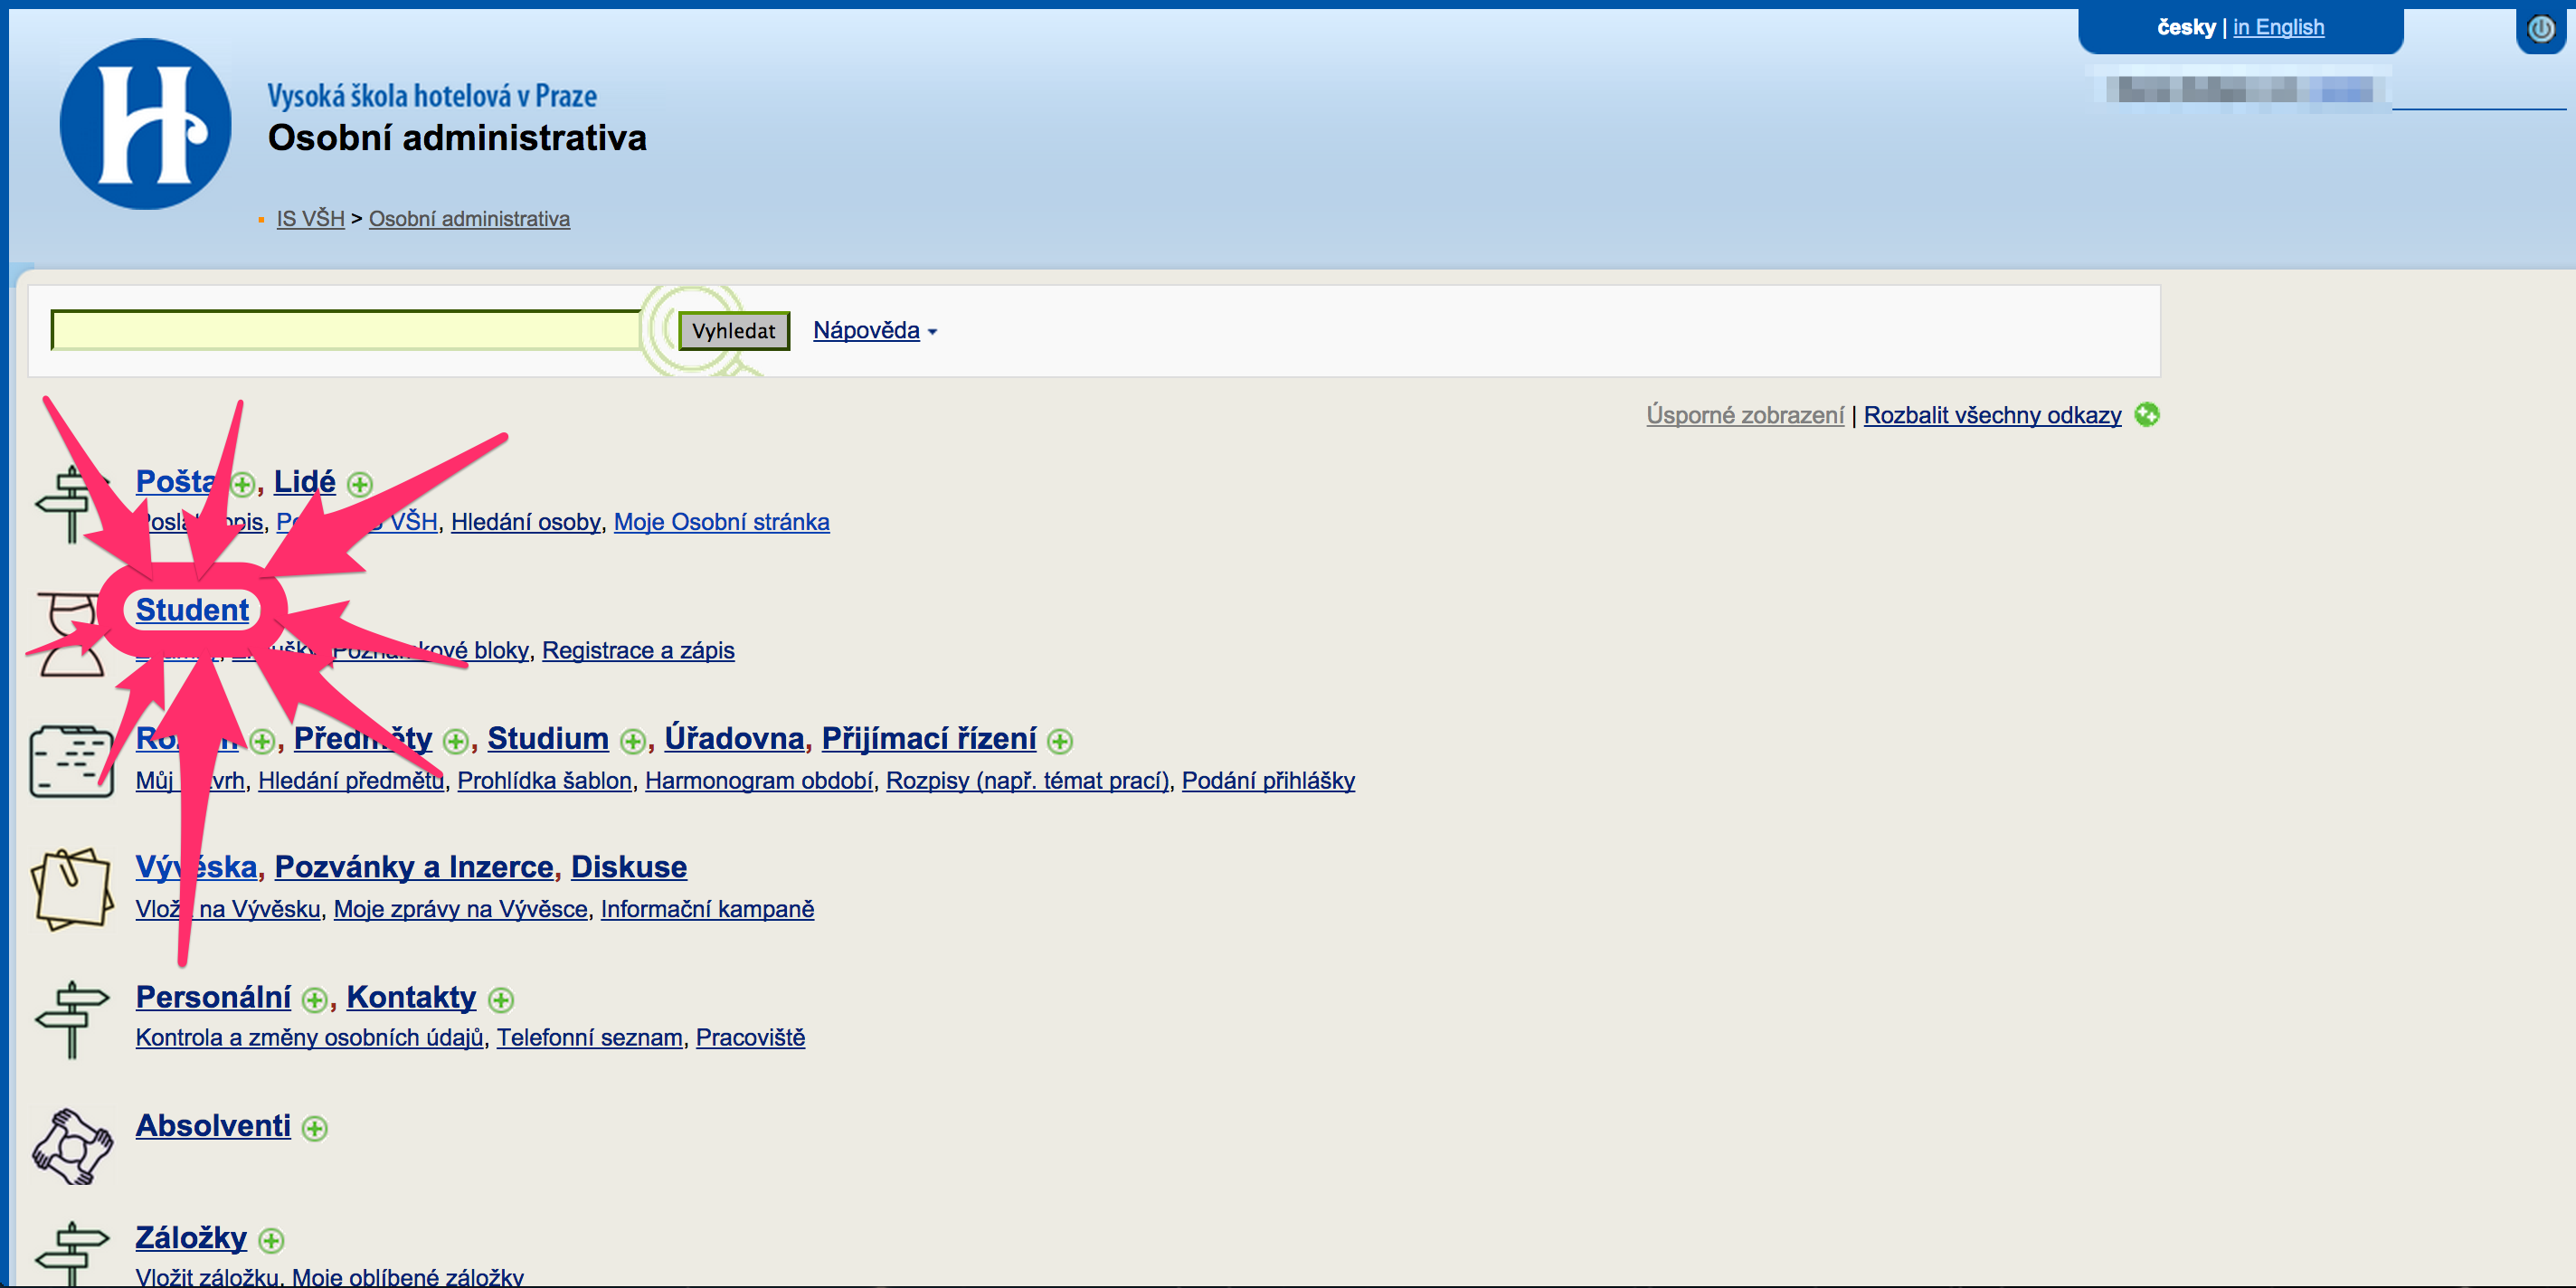
\includegraphics[width=\textwidth]{s17} \\

V této sekci uvidíte své předměty.

Školné lze nalézt kliknutím na odkaz
\textbf{Evidence plateb studenta} přímo uprostřed.

Své známky jsou k dispozici,
pokud stisknete odkaz 
\textbf{Známky za celé studium, získané kredity a stud. průměr}. \\

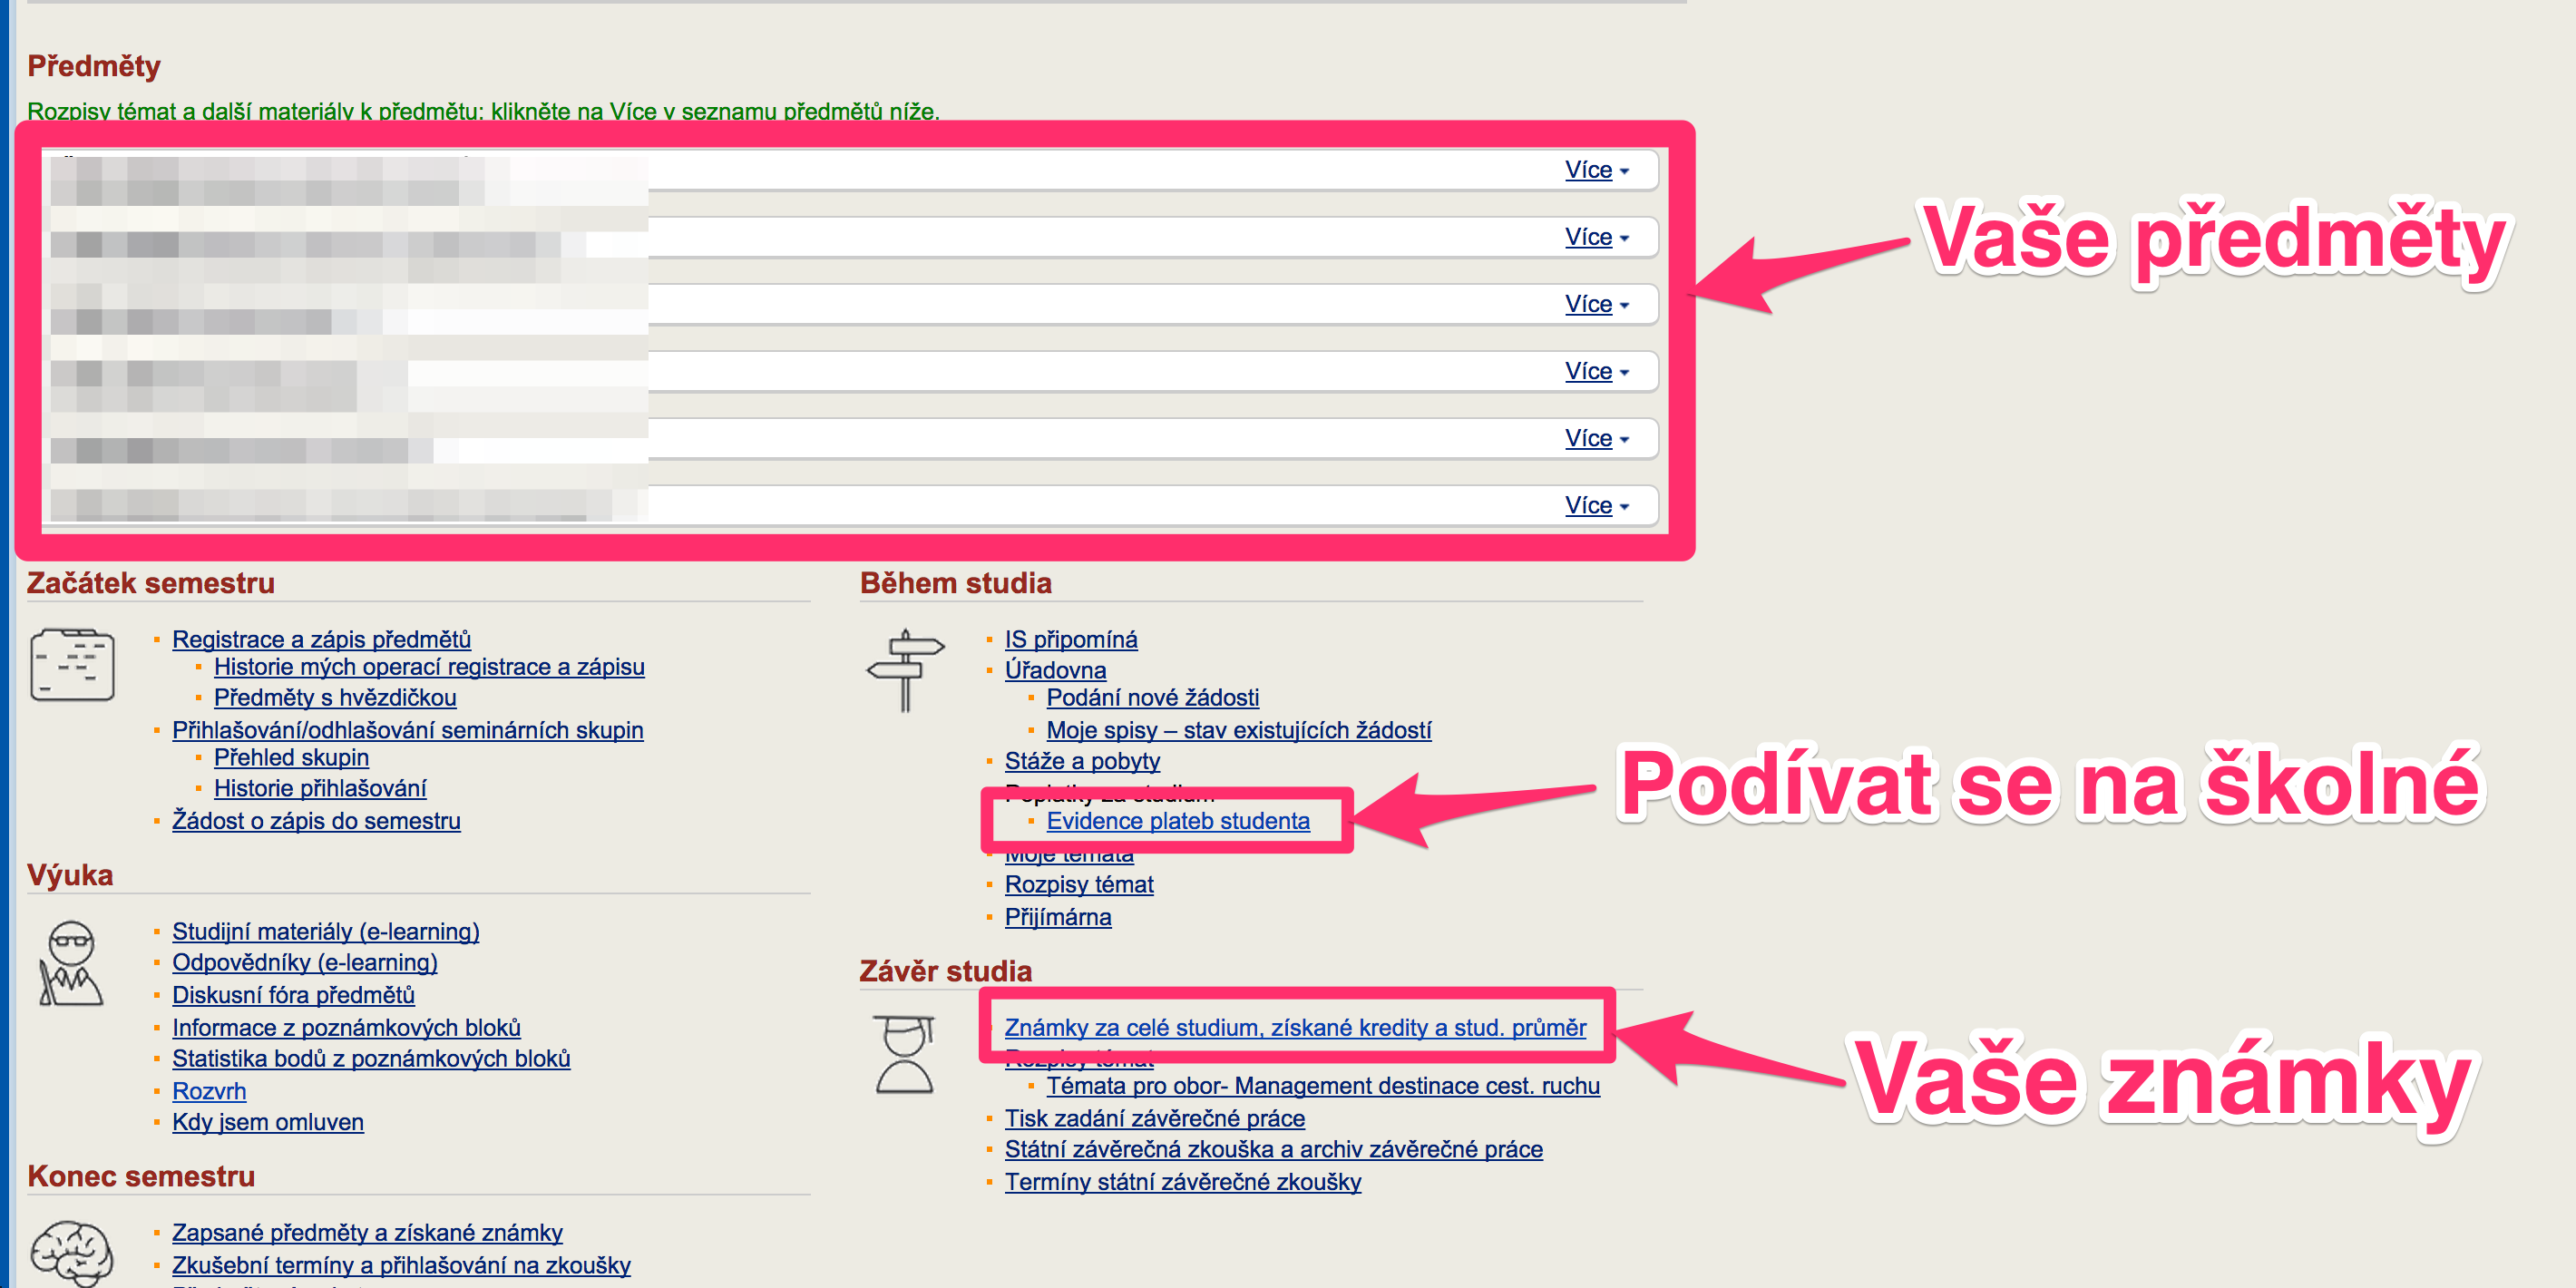
\includegraphics[width=\textwidth]{s18-1} \\

\newpage

Také na začátku roku, můžete být vyzváni k registraci v novém školním roce v oddílech
\textbf{Registrace a zápis předmětů} a \textbf{Zapsané předměty a získané známky}.

O to upozorní ve studentském oddilu, v sekci
\textbf{Vývěska - \href{https://is.vsh.cz/auth/bb/skola/studijni/}{Studijní odd.}} \\

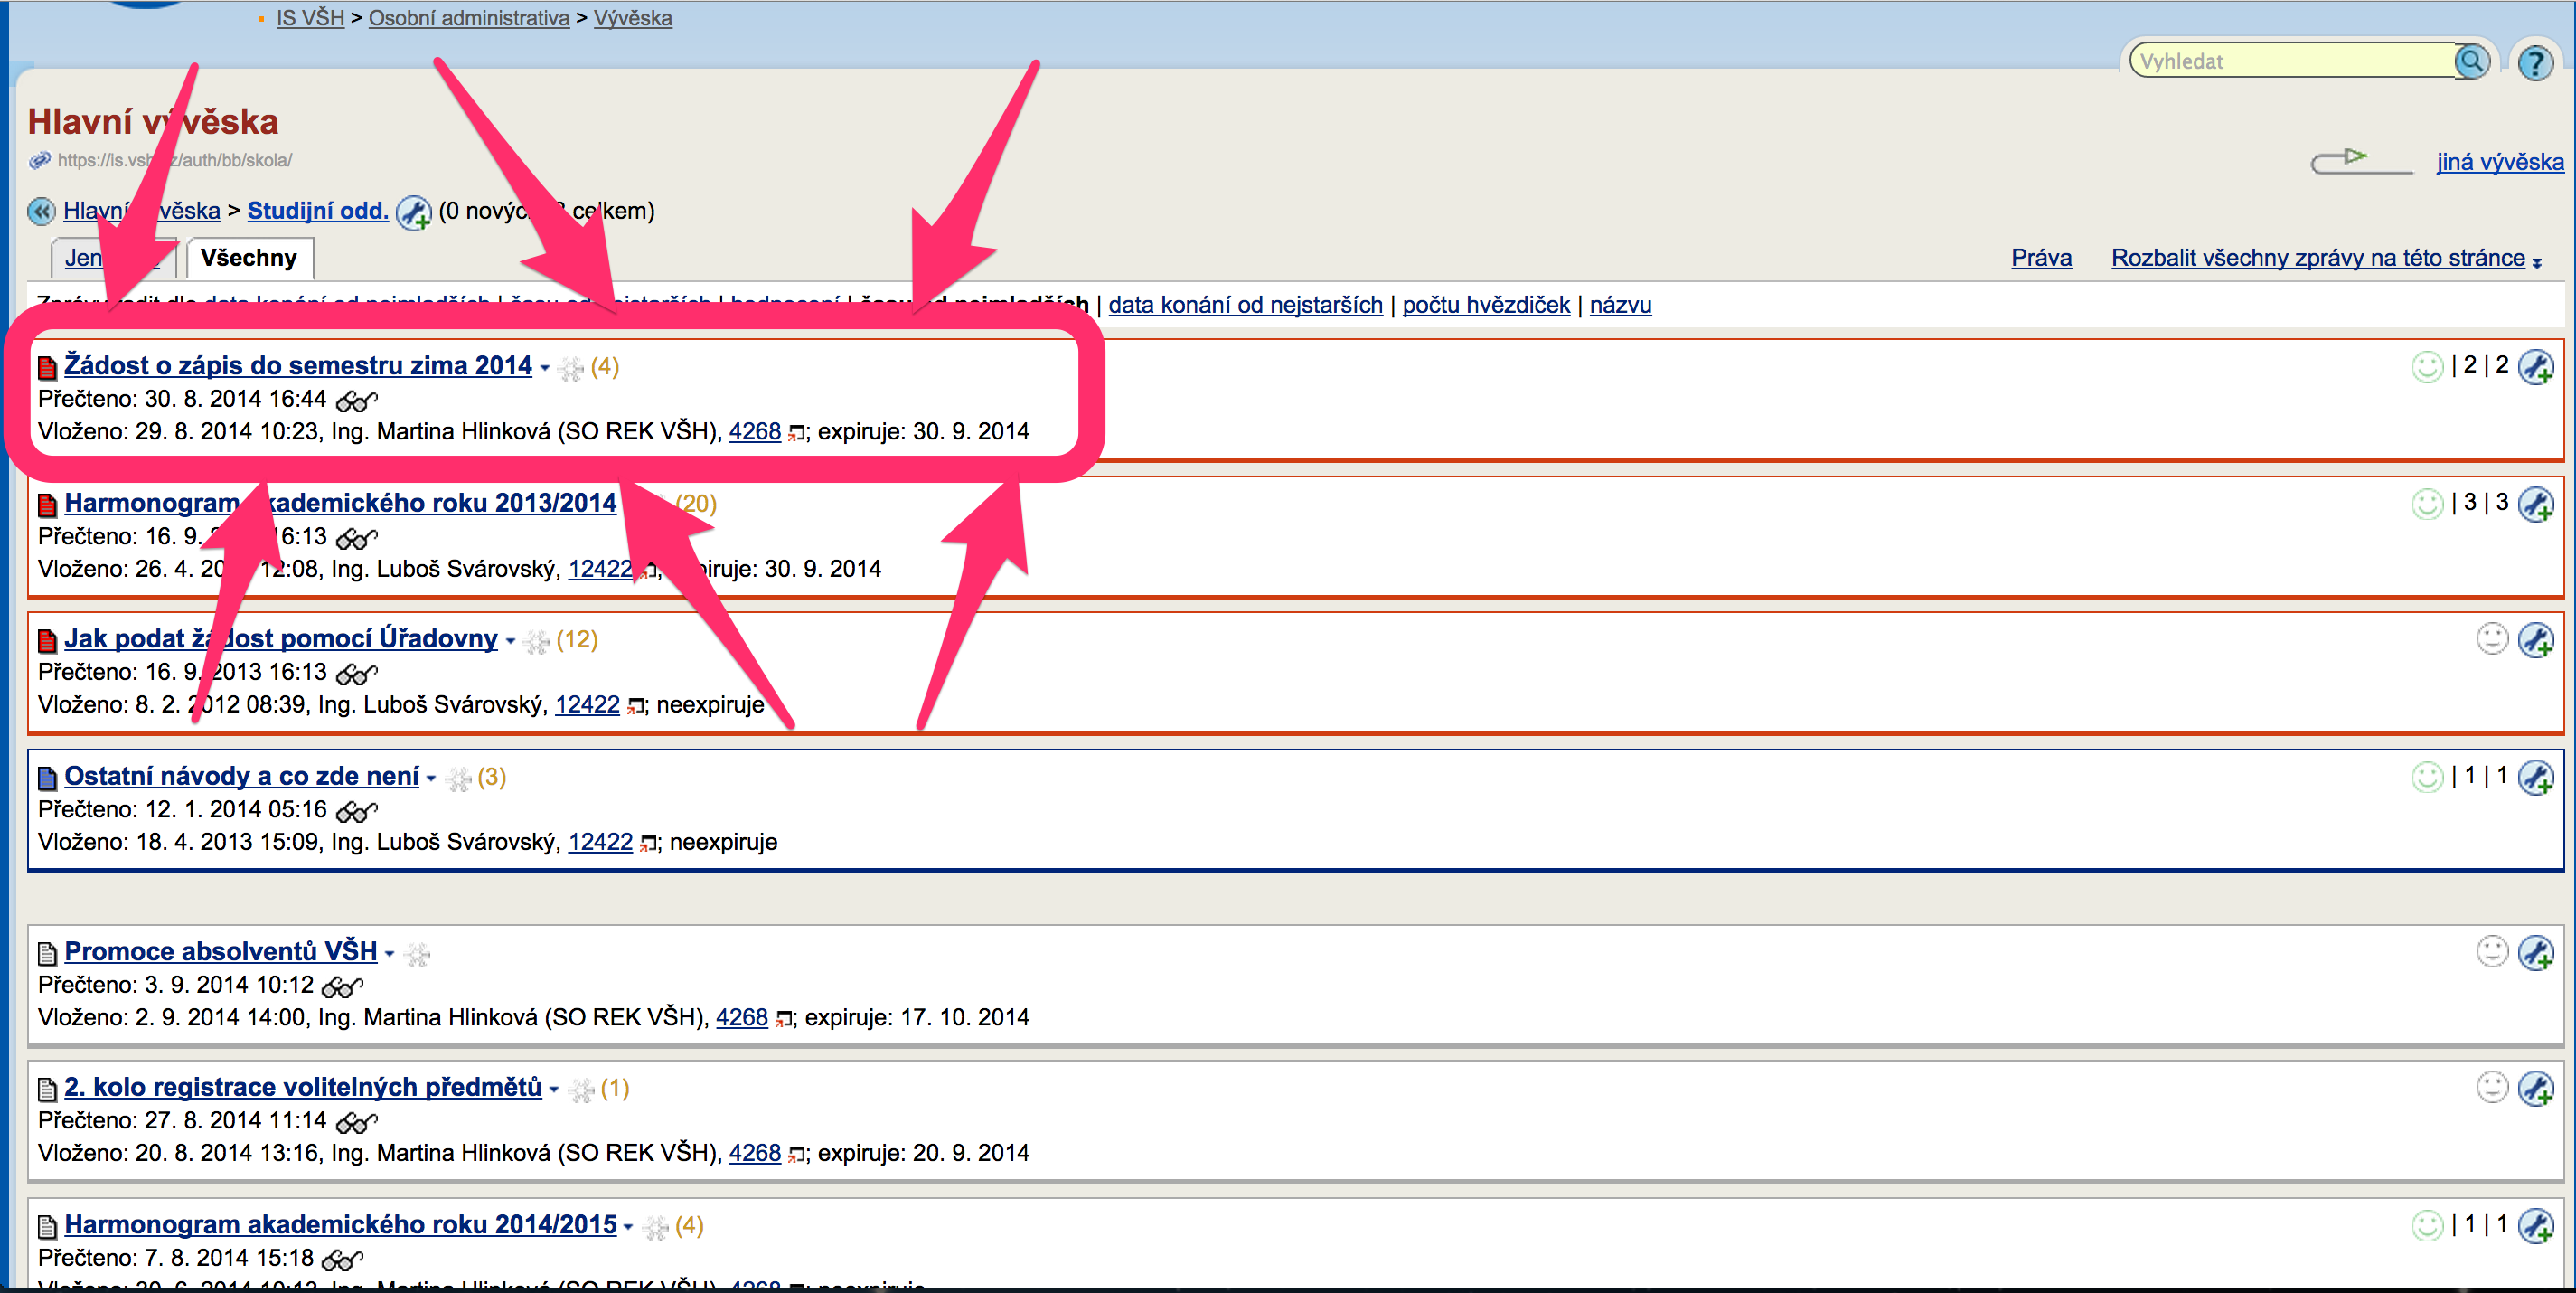
\includegraphics[width=\textwidth]{s19} \\

\newpage

\section{Hledání}

Systém vyhledávání pomocí zadaného řádku na obrázku. \\

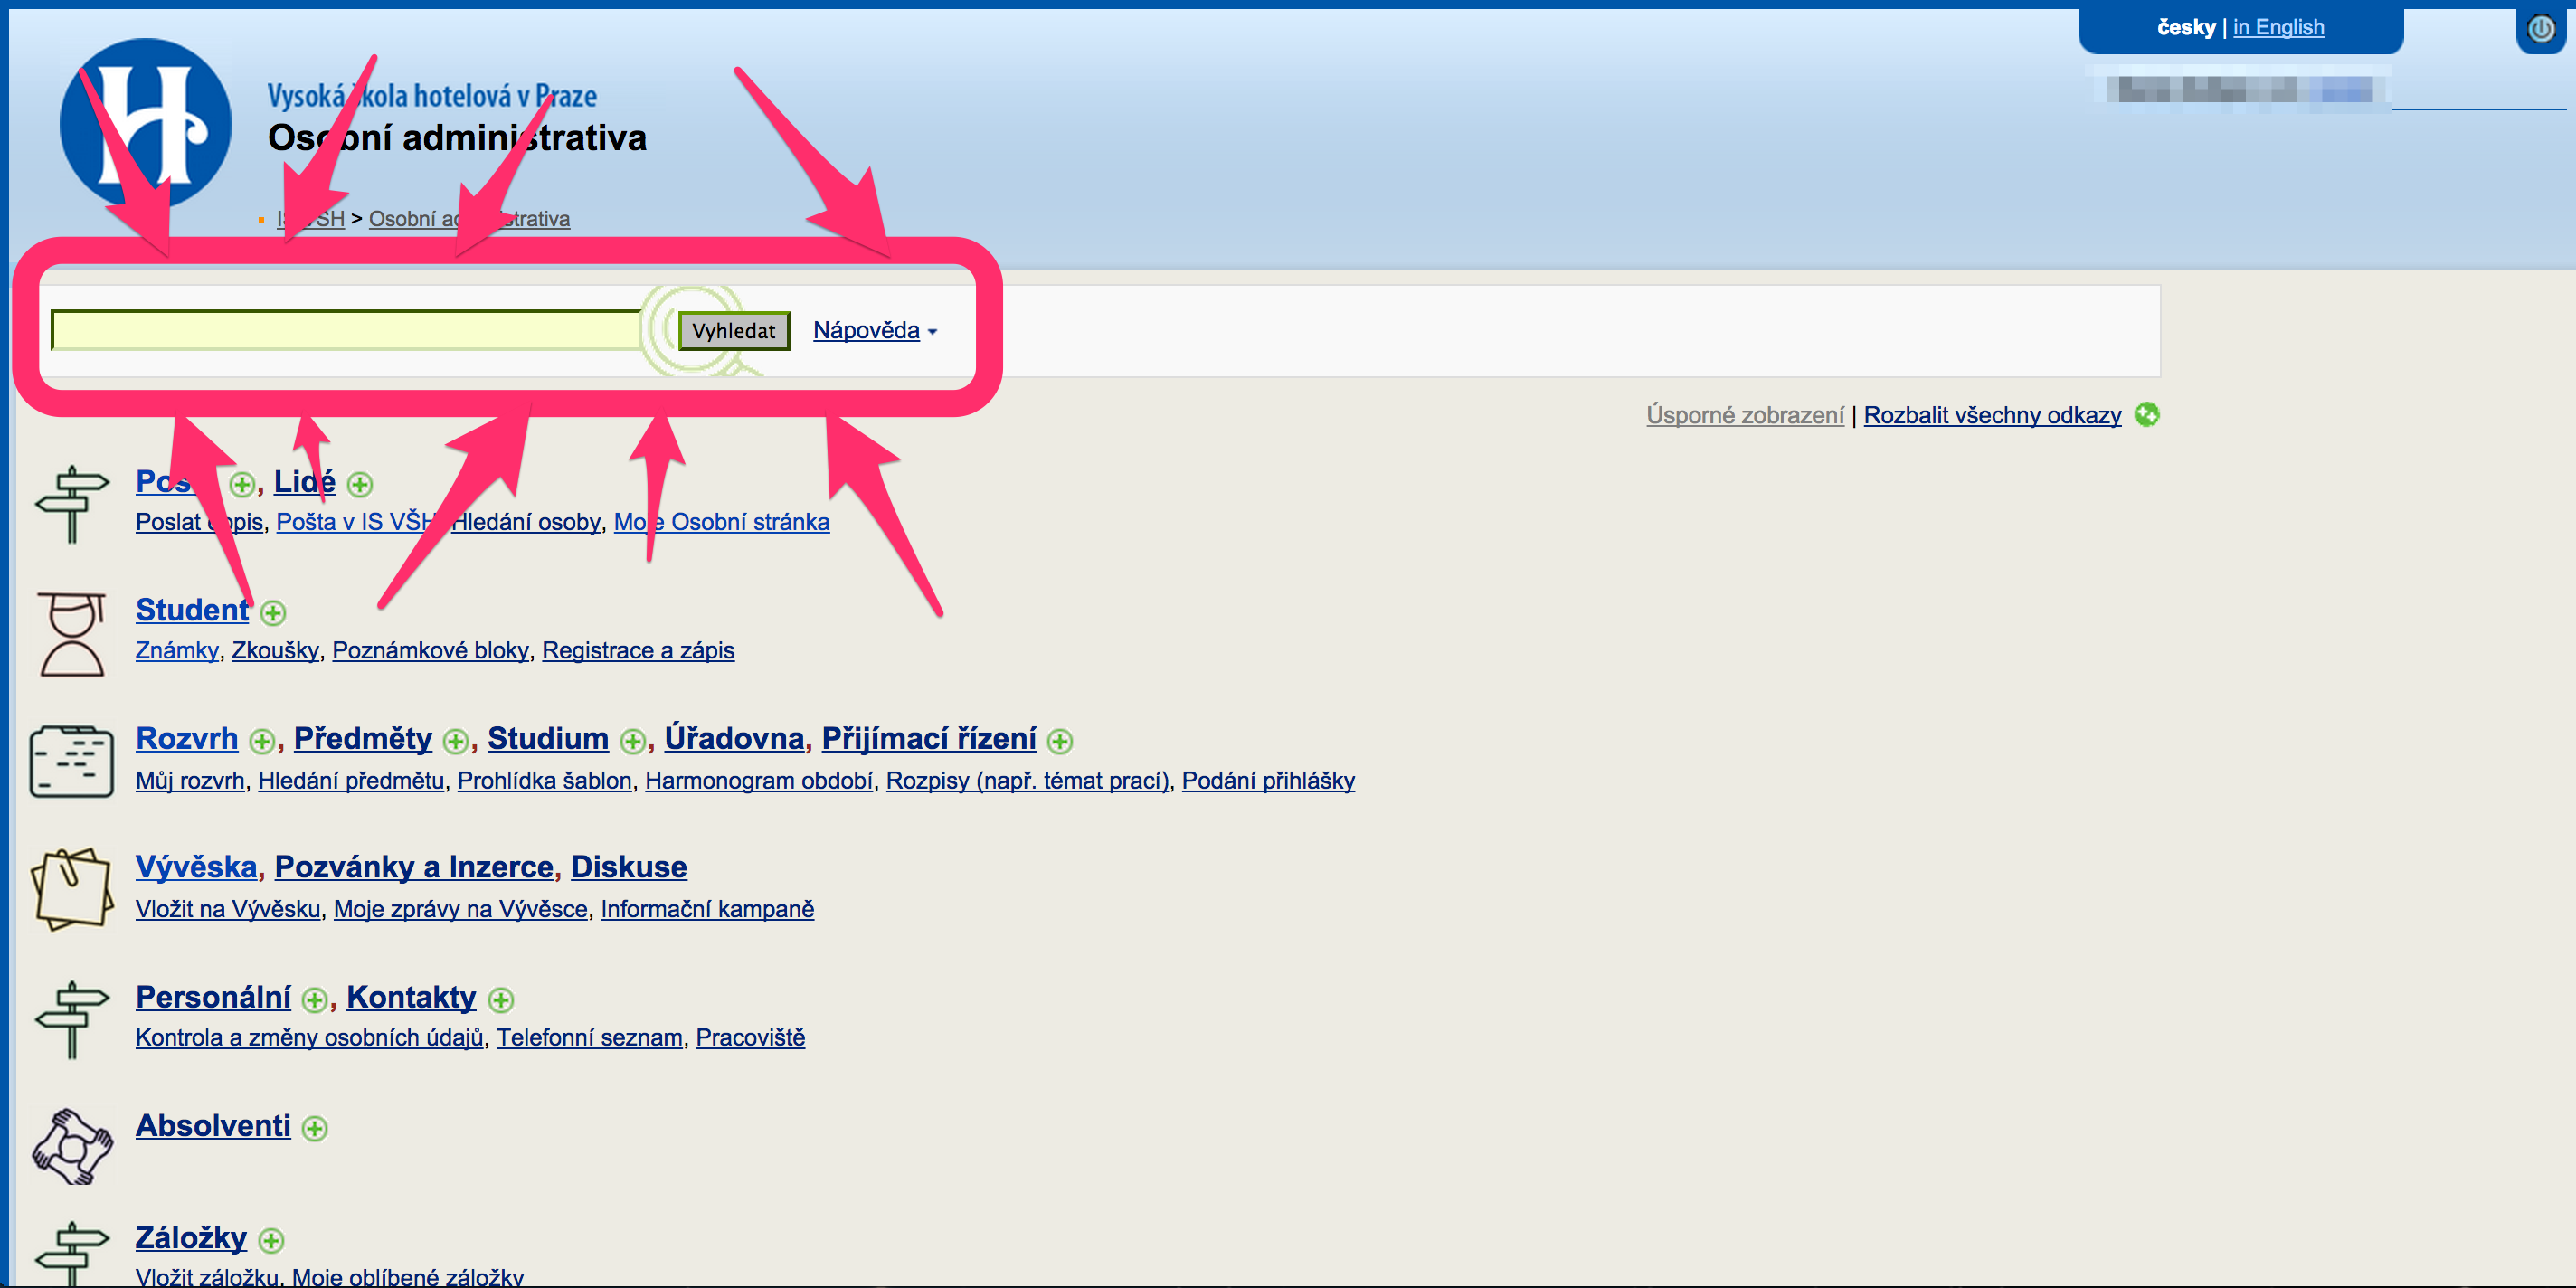
\includegraphics[width=\textwidth]{s20} \\

Napište v řetězec požadované slovo a stiskněte tlačítko \textbf{Enter}, 
a budete přesměrováni na stránku s výsledky.

Chcete-li najít vzdělávací materiály, vyberte oddíl \textbf{Studijní materiály}. \\

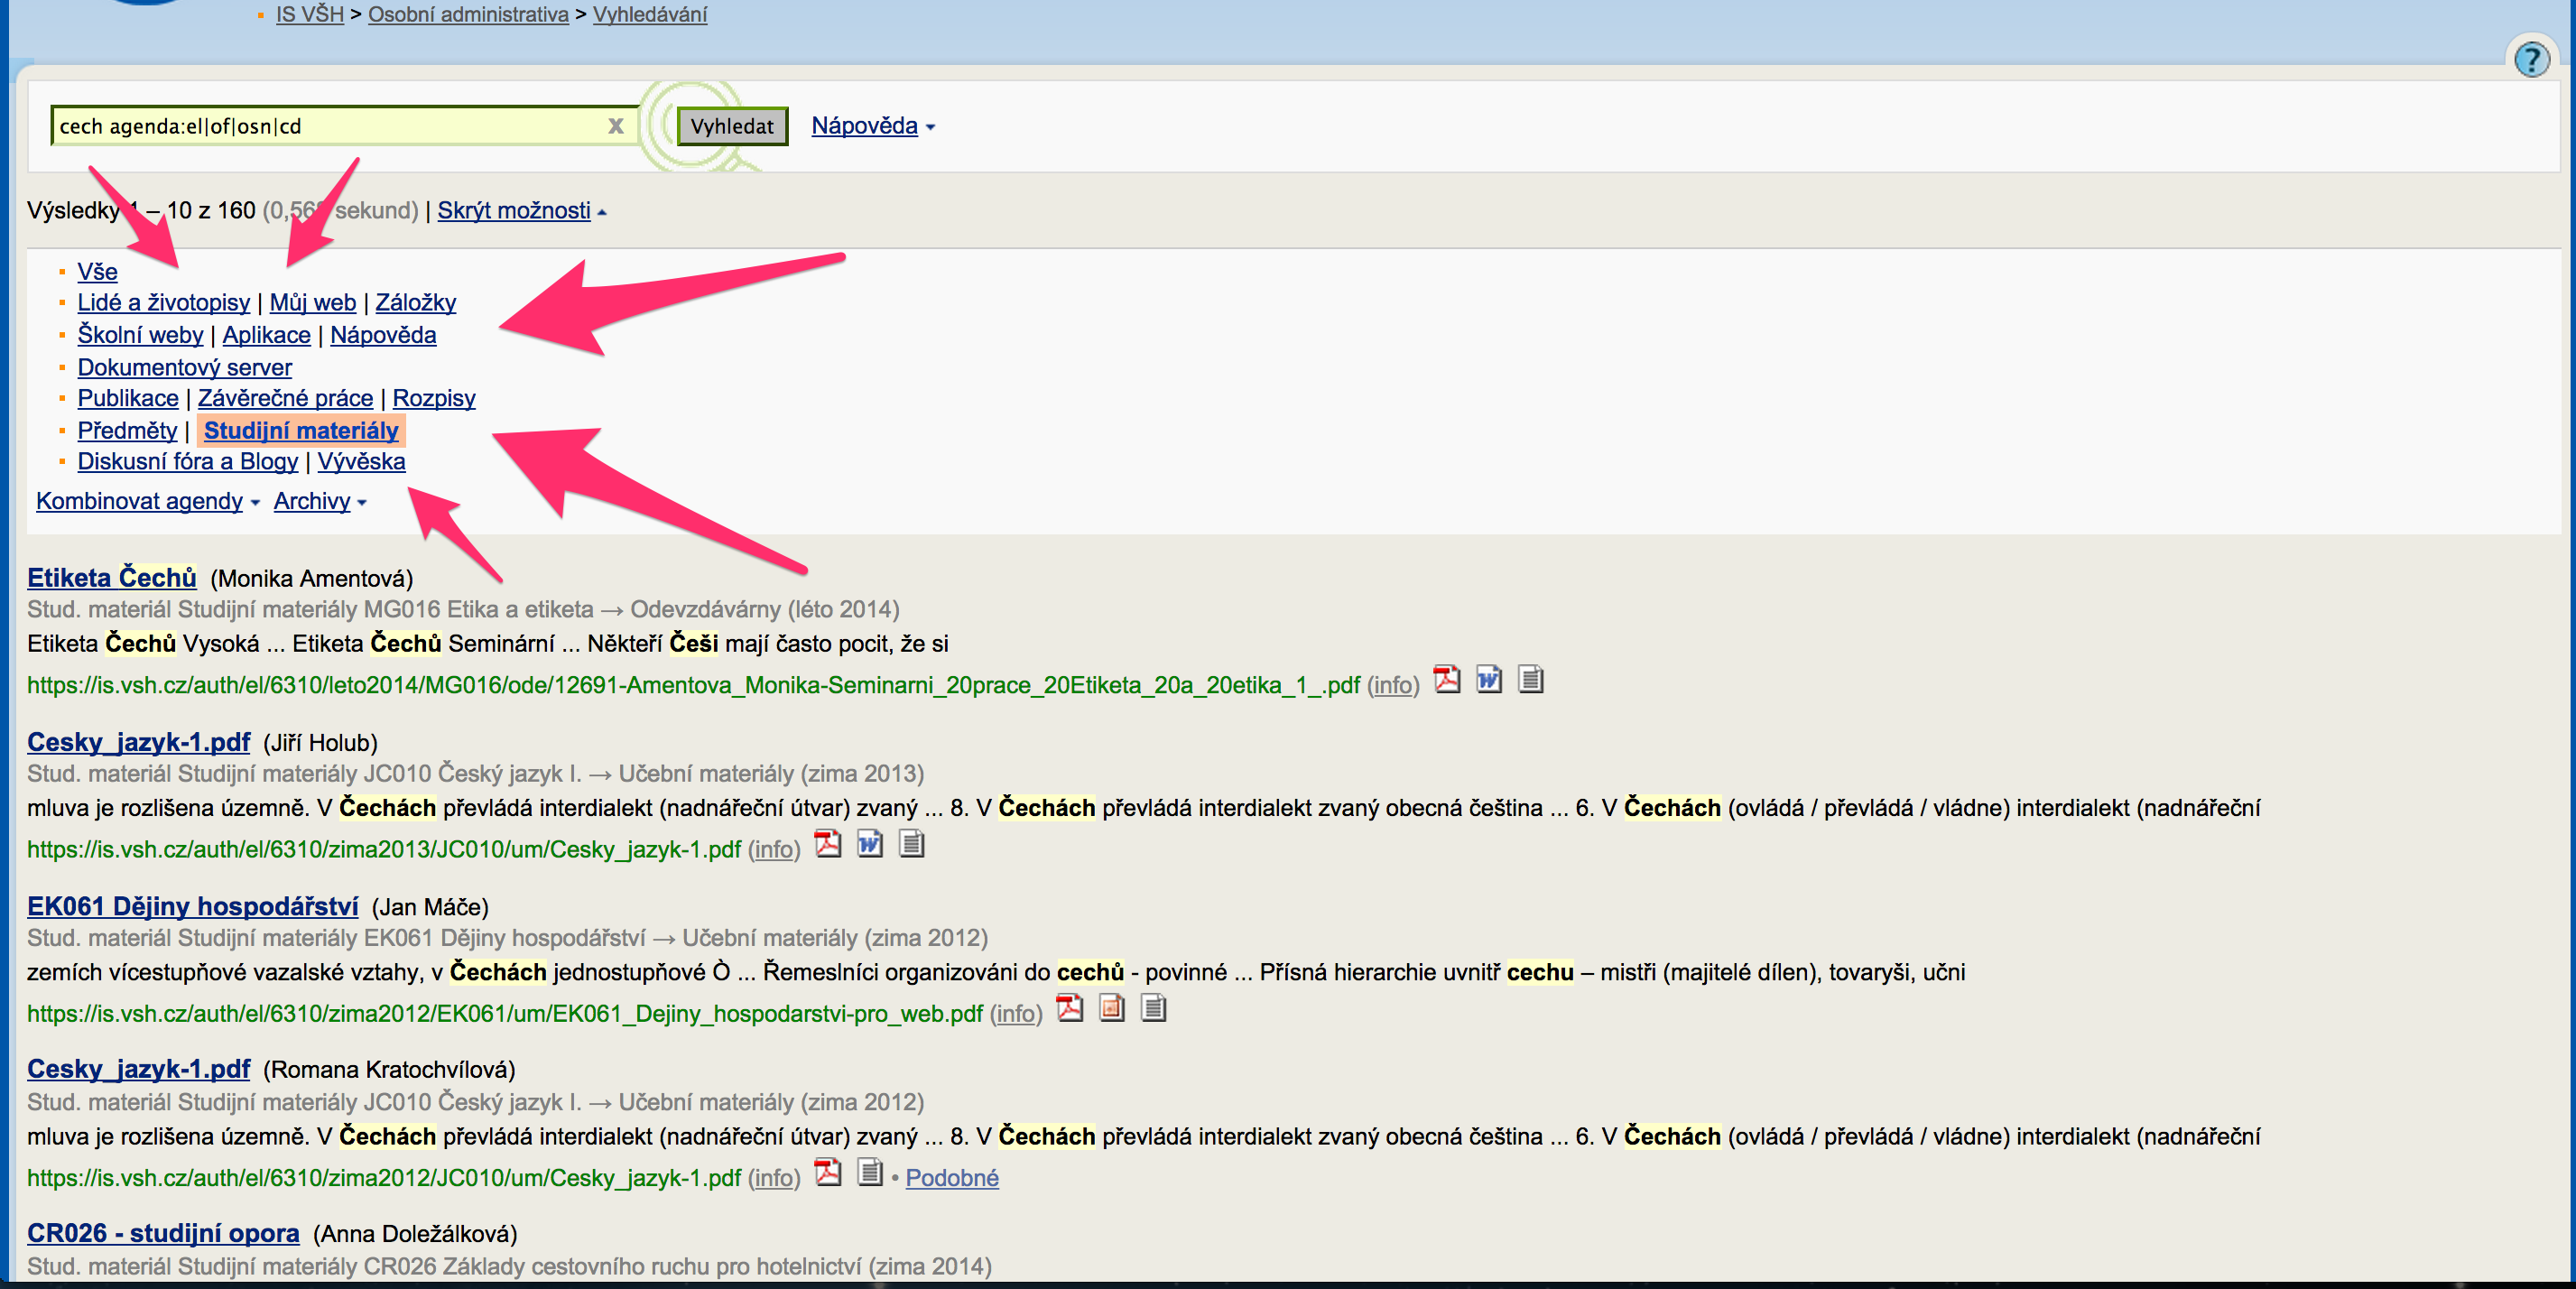
\includegraphics[width=\textwidth]{s21} \\

\newpage

\section{Závěr}

Doufám, že tahle malá příručka bude pro vás užitečná. \\
Děkuji, a přeju vám hodně štěstí!

\end{document} % конец документа